\documentclass[11pt,a4paper]{article}
\usepackage[utf8]{inputenc}
\usepackage[T1]{fontenc}


\usepackage{amsmath,amssymb,amsthm}
\usepackage{booktabs}
\usepackage{array}
\usepackage{multirow}
\usepackage{graphicx}
\usepackage{tikz}
\usetikzlibrary{arrows.meta,positioning,shapes.geometric,calc}
\usepackage{listings}
\usepackage{xcolor}
\usepackage{geometry}
\geometry{margin=2.6cm}
\setlength{\emergencystretch}{3em}
\usepackage[colorlinks=true,linkcolor=blue!50!black,citecolor=blue!50!black,urlcolor=blue!50!black,linktoc=all,bookmarks=true,bookmarksopen=true,bookmarksnumbered=true]{hyperref}

\theoremstyle{plain}
\newtheorem{theorem}{Theorem}
\newtheorem{proposition}{Proposition}
\newtheorem{corollary}{Corollary}
\theoremstyle{definition}
\newtheorem{definition}{Definition}
\theoremstyle{remark}
\newtheorem{remark}{Remark}
\newtheorem{example}{Example}

\lstset{
  language=Python, basicstyle=\ttfamily\scriptsize, breaklines=true, breakatwhitespace=false,
  columns=fullflexible, keepspaces=true, showstringspaces=false, tabsize=4,
  frame=single, framerule=0.3pt, rulecolor=\color{black!40},
  numbers=left, numberstyle=\tiny\color{black!50}, numbersep=6pt,
  commentstyle=\color{black!60}\itshape, keywordstyle=\color{blue!60!black}\bfseries,
  stringstyle=\color{red!50!black}, captionpos=t, aboveskip=1.2em, belowskip=1.2em
}

\newcommand{\R}{\mathbb R}
\newcommand{\Cx}{\mathbb C}
\newcommand{\im}{\operatorname{im}}
\newcommand{\rank}{\operatorname{rank}}
\newcommand{\tr}{\operatorname{tr}}
\newcommand{\diag}{\operatorname{diag}}
\newcommand{\vecop}{\operatorname{vec}}
\newcommand{\spn}{\operatorname{span}}
\newcommand{\T}{\top}

\title{Oblique-Projector Recurrences, Multiplicative Units\\ and an Analytic Discriminant Block\\[2mm]
\large Exact expressive limits, capacity results and calibrated rank selection\\ for recursive oblique projection networks (ROPN)\\[1mm]
\normalsize A technical report: theorems, worked examples, experiments and code}
\author{Olivier Caspary \\
    Universit\'e de Lorraine, LCOMS, F-57000 Metz, France \\
    \small{\emph{olivier.caspary@univ-lorraine.fr}}}
\date{\today}

\begin{document}
\maketitle

\begin{abstract}
A recursive oblique projection network (ROPN) is a residual network whose
linear maps are oblique projectors $P=U(W^\T U)^{-1}W^\T$: a
\emph{representation} subspace $\im U$ and a \emph{measurement} subspace
$\im W$ that need not coincide. We characterise exactly the expressive limits
of recurrences built on oblique projectors, establish capacity results for
multiplicative units, and construct an analytic discriminant realisation
with calibrated rank selection. \emph{Recurrences.} For a shared oblique
block, the linear recursion collapses to $I+c_LP$; the oblique code is
invariant under the scalar-gated recursion, whose gate is constant along
the orbit when it reads inside $\spn(W)$; the gated block has an explicit
Jacobian determinant; and with $r$ code coordinates and $m$ independent
gate directions in the kernel, the non-linearity has at most $r+m$ linear
functionals of the input as arguments, whatever the number of steps. Depth
therefore does not enlarge the information accessible to the non-linearity;
it can still change the function computed on it. \emph{Multiplicative
units.} A gated unit with decoupled gate and value directions (the
triceptron, a gated linear unit) contains SiLU units, has ReLU units as
uniform limits, approximates every quadric of inertia $(p,n)$ at fixed
width $\max(p,n)$, and obeys the cell-count bound of a ReLU layer; a ReLU
layer needs a width that grows with the accuracy required on a disc. With
the same trainer for both families, the minimal widths predicted by the
theorem are observed, and no accuracy difference between the two families
is established beyond about thirty parameters. \emph{Analytic discriminant block.} The
Fisher generalised eigenproblem gives a biorthogonal pair $(U,W)$ and an
exactly idempotent projector; with a centroid read-out the block is exactly
linear discriminant analysis (LDA) with the same covariance estimate, an
equivalence stated explicitly and used throughout. Its specific content is
an exact $C\times C$ factorisation with a dual form for $n<d$, a bound on
the projector norm through the condition number of the metric, and a rank
selection in which the structural, tested and used ranks are kept apart:
the permutation test in a label-free metric is calibrated under the global
null hypothesis, a sequential variant is evaluated under alternatives of
every rank, and a min-$p$ procedure controls the family-wise error across
blocks. The tested rank is a detection statement, not a risk-optimal
choice: in our experiments, using the structural rank $C-1$ for prediction
was within $0.2$ accuracy point of using the true rank, whereas using a
tested rank cost up to nine points when the test lacked power. \emph{Evidence.} The theorems are proved; the experiments use
synthetic data and small public datasets, with paired comparisons,
confidence intervals and a pre-specified equivalence margin. In them the
block is equivalent to shrinkage LDA, as it must be, ahead of logistic
regression and MLP baselines on small near-Gaussian samples, tuned or not,
and behind the MLP on the real digits data from thirty samples per class
(behind logistic regression at one hundred).
Gradient fine-tuning of the block, including variants in which both
subspaces move, showed no net gain in the protocol tested. No experiment on
real EEG data is reported. Exploratory extensions (lattices, Kronecker
metrics, kernels, the SPD manifold, Fourier operators) are collected in
appendices and carry no general claim. The complete \texttt{numpy} code and
the logs of every experiment are included.
\end{abstract}

\tableofcontents
\newpage

%% =====================================================================
\section{Introduction}
\label{sec:intro}
%% =====================================================================

\subsection{Scope and positioning}
Oblique projection networks replace the linear maps of a residual network
by oblique projectors and are normally trained by gradient descent, with
gates that select the rank of each block and the depth of the stack. This
report studies what can be said \emph{exactly} about such networks, and
what can be built \emph{without} back-propagation. It does not propose a
new architecture, and it does not claim an empirical advantage over
established classifiers. Its three contributions are of different natures
and are kept apart throughout.
\begin{enumerate}
  \item \textbf{Exact expressive limits of oblique-projector recurrences}
  (Section~\ref{sec:recursion}). For a shared block built on one projector,
  four results describe what repeated application can and cannot do:
  collapse of the linear recursion (Theorem~\ref{thm:collapse}), invariance
  of the code and constancy of a gate reading inside $\spn(W)$
  (Proposition~\ref{prop:code}), an explicit Jacobian determinant
  (Theorem~\ref{thm:gate-det}), and the reduction of the arguments of the
  non-linearity to $r+m$ linear functionals (Theorem~\ref{thm:A}). The
  precise conclusion is: \emph{depth does not enlarge the subspace of
  information accessible to the non-linearity; it can nevertheless modify
  the function computed on that subspace}.
  \item \textbf{Capacity results for multiplicative units}
  (Section~\ref{sec:tri}). Theorem~\ref{thm:B} gives the inclusion of
  SiLU/ReLU units, the exact number of units needed for a quadric, a cell
  count, and a necessary width for ReLU layers on a disc. The experiments
  of that section use the same trainer for gated and ReLU networks, with
  and without the linear skip of the theoretical construction.
  \item \textbf{An analytic discriminant realisation with calibrated rank
  selection} (Sections~\ref{sec:block}--\ref{sec:rank}). The block is the
  Fisher discriminant written as an oblique projector. With a centroid
  read-out it is \emph{exactly} LDA with the same covariance estimate
  (Proposition~\ref{prop:lda}); what is specific is the exact $C\times C$
  factorisation and its dual form (Proposition~\ref{prop:dual}), the
  control of the projector norm by the metric
  (Proposition~\ref{prop:metric-bound}), and a rank selection whose
  calibration is established under the global null hypothesis and measured
  under alternatives (Section~\ref{sec:rank}).
\end{enumerate}
Three ingredients of the block must not be confused
(Section~\ref{sec:ingredients}): the \emph{Fisher metric} is what brings
prediction accuracy; the \emph{factorisation} is what brings computational
savings; \emph{idempotence} brings exact structural statements (the
theorems above, the norm identities) and no accuracy by itself.

\subsection{Status of the claims}
\begin{center}\small\renewcommand{\arraystretch}{1.15}
\begin{tabular}{@{}p{0.31\linewidth}p{0.31\linewidth}p{0.31\linewidth}@{}}
\toprule
\textbf{Proved} & \textbf{Measured, in the stated protocols} & \textbf{Suggested, not established} \\
\midrule
Theorems~\ref{thm:collapse}--\ref{thm:B},
Propositions~\ref{prop:code}--\ref{prop:metric-bound} and their
corollaries; exact level of the permutation test under the global null
hypothesis; exact equivalence of the block with LDA. &
Calibration and rank recovery (Section~\ref{sec:rank}); accuracy relative
to LDA, logistic regression and MLPs with paired confidence intervals
(Section~\ref{sec:central}); timings; small-sample diagnosis and
fine-tuning (Section~\ref{sec:small}); parity of gated and ReLU networks
under one trainer (Section~\ref{sec:tri}). &
Usefulness on real EEG data (not tested); behaviour of the extensions of
Appendices~\ref{sec:extensions}--\ref{sec:fourier} beyond the favourable
synthetic cases examined; any statement about well-tuned large networks. \\
\bottomrule
\end{tabular}
\end{center}
An absence of measured gain is reported as such (``no net gain observed in
the protocol tested''), never as a proof of uselessness; a difference
smaller than its uncertainty is reported as undetermined, not as an
equality (Section~\ref{sec:central} gives the convention).

\subsection{Terminology}
\emph{Back-propagation-free} qualifies the programme as a whole: no
parameter is obtained by gradient descent. \emph{Analytic} is reserved for
sub-problems solved by a finite sequence of standard linear-algebra
operations with no tuning loop: the block given its covariance estimate,
the $C\times C$ reduction, the centroid read-out. Several components of the
appendices are back-propagation-free without being analytic (the Karcher
mean, the alternating estimation of a Kronecker metric, internal
cross-validation). \emph{Rank selection} replaces the looser
``self-sizing'': the \emph{structural} rank is the bound $\min(C-1,d)$, the
\emph{tested} rank is the output of a statistical rule and may be zero, the
\emph{used} rank is the one the classifier actually employs.

\subsection{Notation}
Data $x\in\R^d$, $n$ training samples, $C$ classes with sizes $n_c$, class
means $\mu_c$, grand mean $\bar\mu$. Within-class scatter
$S_W=\tfrac1n\sum_c\sum_{i\in c}(x_i-\mu_c)(x_i-\mu_c)^\T$ (pooled; the
unshrunk baseline of Section~\ref{sec:small} divides by $n-C$ instead of
$n$), between-class scatter
$S_B=\sum_c n_c(\mu_c-\bar\mu)(\mu_c-\bar\mu)^\T/(C-1)$ (of rank at most
$C-1$), total scatter
$S_T=\tfrac1n\sum_i(x_i-\bar\mu)(x_i-\bar\mu)^\T=S_W+\tfrac{C-1}{n}S_B$,
which does not depend on the labels. An oblique projector of
rank $r$ is $P=U(W^\T U)^{-1}W^\T$ with $U,W\in\R^{d\times r}$ of full rank
and $W^\T U$ invertible; in biorthogonal form $W^\T U=I_r$ and $P=UW^\T$.
The \emph{code} of $h$ is $c=W^\T h\in\R^r$ and its \emph{residual} is
$\rho=(I-P)h\in\ker P$, so that $h=Uc+\rho$ uniquely. A projector is
$M$-orthogonal for a positive definite $M$ when $W=MU$; the Fisher block is
$S_W^{-1}$-orthogonal, hence oblique in the Euclidean sense and orthogonal in
the Fisher metric. $\sigma$ denotes the logistic sigmoid; $\kappa(S_W)$ the
condition number of the within-class scatter, used as an anisotropy knob in
the synthetic experiments; ``LW'' the Ledoit--Wolf shrinkage estimator. All
experiments use \texttt{numpy}, \texttt{scipy} and \texttt{scikit-learn}
only; every gradient used in the comparisons is written by hand and verified
by finite differences. Unless stated otherwise, accuracies are test accuracies
on stratified $70/30$ splits, reported as mean $\pm$ standard deviation over
seeds (the number of seeds is given with each table). In
Sections~\ref{sec:rank}, \ref{sec:central}, \ref{sec:small},
\ref{sec:stability} and~\ref{sec:audit}, and in Table~\ref{tab:tri}, every
seed draws a new synthetic dataset; in the benchmark tables of
Appendices~\ref{sec:bench}, \ref{sec:lattice}, \ref{sec:alternatives}
and~\ref{sec:crossgram} and in Table~\ref{tab:tri-all} each dataset
(synthetic or real) is fixed and the seeds are five different splits, so
that the small synthetic cases rest on $5\times18$ test predictions and
their standard deviations measure split variability only.
Appendices~\ref{sec:riemann} and~\ref{sec:fourier} use unstratified $50/50$
splits of independent draws. Comparisons between methods in
Sections~\ref{sec:tri}, \ref{sec:rank}, \ref{sec:central}
and~\ref{sec:small} are paired on the same realisations and reported with a
$95\%$ interval and a verdict relative to an equivalence margin of one
accuracy point (convention in Section~\ref{sec:central}). The tables of the
appendices report means and standard deviations only: there, differences
smaller than the quoted standard deviations must be read as undetermined. Timings are wall-clock times on the CPU of the execution sandbox, vary
from run to run, and are indicative only. Shrinkage follows Ledoit and
Wolf~\cite{ledoitwolf2004}. A few symbols are reused with a local meaning,
always stated where it applies: $L$ is the residual scale (and number of
steps) of a recursion, $T$ a number of recursion steps (the number of time
samples of a trial in Appendices~\ref{sec:kron} and~\ref{sec:riemann}), $M$ a
generic metric (the $C\times C$ matrix $D^\T S^{-1}D$ in
Section~\ref{sec:fast}), $\mu$ without index the Ledoit--Wolf target scale
$\tr S_W/d$, and $a$ either the gate value or the Ledoit--Wolf intensity.

%% =====================================================================
\section{Oblique projectors: definitions and geometry}
\label{sec:prelim}
%% =====================================================================
Figure~\ref{fig:geometry} shows the object this report is about, in the
plane. An oblique projector is determined by two subspaces: its image
$\spn(u)$, where the projected points land, and its kernel $\spn(w)^\perp$,
the direction \emph{along which} points are moved to the image. The
measurement direction $w$ is orthogonal to the kernel, not to the image: the
code $w^\T x$ reads how much of $x$ lies ``across'' the kernel, and $Px=u\,w^\T x$
places that amount on the image. When $w\propto u$ the projector is
orthogonal and $Px$ is the nearest point of the image; otherwise $Px$ is
further from $x$ than the orthogonal projection by at most the factor
$\|P\|_2=1/\sin\theta_{\min}$ (Section~\ref{sec:stability}), and the same
factor bounds the amplification of input perturbations. In a classifier the
image is where the class means differ and the kernel is where the
within-class noise lives: an oblique projector can discard noise directions
that are \emph{not} orthogonal to the signal, which an orthogonal projector
cannot.

A second reading, due to Rocks and Mehta~\cite{rocksmehta2021} in the
context of over-parameterised regression, is useful throughout this report.
Write $P=Q_U(Q_W^\T Q_U)^{-1}Q_W^\T$ with orthonormal bases $Q_U$, $Q_W$ of
the image and of the measurement subspace. Since $Q_W^\T x=Q_W^\T(Q_WQ_W^\T x)$,
the projection proceeds in \emph{two steps}: $x$ is first projected
\emph{orthogonally} onto the measurement subspace $\spn(W)$, giving
$\hat x_W=Q_WQ_W^\T x$ (the only part of $x$ the block reads: the code
$W^\T x$ depends on $x$ through $\hat x_W$ alone), and $\hat x_W$ is then
re-expressed in the representation subspace $\spn(U)$. The second step is
where obliquity acts: if $\theta_1\le\dots\le\theta_r$ are the principal
angles between $\spn(U)$ and $\spn(W)$, the non-zero singular values of $P$
are exactly $1/\cos\theta_i$, so that each measured direction is stretched by
the factor $1/\cos\theta_i$ on its way to the image, and
$\|P\|_2=1/\cos\theta_r=1/\sin\theta_{\min}$ (the two angles are
complementary, since $\ker P=\spn(W)^\perp$). When $U=W$ all angles vanish,
every factor is one and the projector is orthogonal. Verified on the
analytic block ($d=20$, $C=4$, $\kappa=200$): singular values
$(1.5469,1.4340,1.1861)$ against $1/\cos\theta_i$ for principal angles
$(49.7^\circ,45.8^\circ,32.5^\circ)$, and $W^\T x=W^\T\hat x_W$ to $3\times10^{-16}$.
Figure~\ref{fig:geometry} shows both steps.
\begin{figure}[t]
\centering
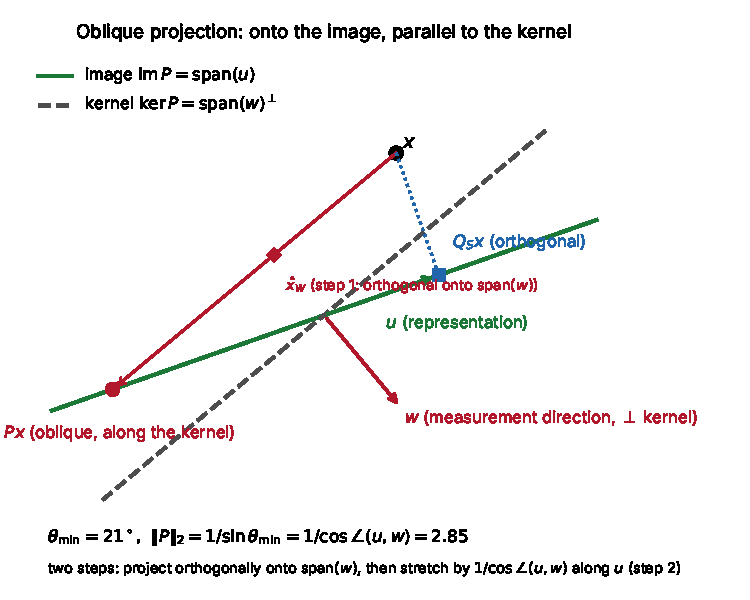
\includegraphics[width=0.62\textwidth]{fig_oblique_geometry.pdf}
\caption{An oblique projector in the plane: image (green), kernel (grey,
dashed), representation direction $u$ and measurement direction $w$ (orthogonal
to the kernel). The point $x$ is sent to $Px$ along the kernel direction; the
orthogonal projection $Q_Sx$ onto the same image is shown for comparison. The
two-step reading: $x$ is first projected orthogonally onto $\spn(w)$
(diamond, $\hat x_W$), then carried to the image with the stretch factor
$1/\cos\angle(u,w)$. The norm $\|P\|_2=1/\sin\theta_{\min}=1/\cos\angle(u,w)$
grows as the kernel approaches the image.}
\label{fig:geometry}
\end{figure}

%% =====================================================================
\section{Exact expressive limits of oblique-projector recurrences}
\label{sec:recursion}
%% =====================================================================

\subsection{Collapse of the linear recursion}
\begin{theorem}[Collapse of a recurrent idempotent oblique block]
\label{thm:collapse}
Let $P=UW^\T$ be idempotent ($W^\T U=I_r$) and
$\mathcal T_L=(I+P/L)^L$ the operator obtained by applying $L$ times the
\emph{same} residual block $h\mapsto h+Ph/L$. Then, for every $L\ge1$,
\begin{equation}
  \mathcal T_L=I+c_L\,P,\qquad c_L=(1+\tfrac1L)^L-1,
  \label{eq:collapse}
\end{equation}
exactly.
\end{theorem}
\begin{proof}
$P$ idempotent induces the oblique direct sum $\R^d=\im P\oplus\ker P$. On
$\ker P$ the block is the identity; on $\im P$ it is multiplication by
$1+1/L$. Hence $\mathcal T_Lx=(I-P)x+(1+1/L)^LPx$.
\end{proof}
Numerically, the brute-force iteration agrees with~\eqref{eq:collapse} to a
relative error below $1.2\times10^{-15}$ for $L\in\{1,\dots,256\}$
($c_1=1$, $c_2=1.25$, $c_4=1.441406$, $c_8=1.565785$, $c_{16}=1.637928$,
$c_{64}=1.697345$, $c_{256}=1.712992$, converging to $e-1$).

\subsection{Invariance of the oblique code under a gated recursion}
It is tempting to believe that a non-linear gate restores genuine depth,
because $\|h_T-h_0\|$ keeps evolving with $T$. The evolution is real, but it
is also in closed form.

\begin{proposition}[Code invariance and gate collapse]
\label{prop:code}
Let $h_{t+1}=(1-a_t)h_t+a_tPh_t$ with $a_t=\sigma(s^\T h_t+b)$ (shared
weights).
\begin{enumerate}
  \item[(i)] \textbf{Code invariance.} For every $T$ and every sequence
  $(a_t)$: $W^\T h_T=W^\T h_0$. The recursion moves $h$ only along
  $\ker W^\T$, the direction \emph{along which} one projects.
  \item[(ii)] \textbf{Gate collapse.} If $s\in\spn(W)$ (the analytic gate,
  $s\propto w_1$), then $a_t=a_0=:a(x)$ for all $t$ and
  \begin{equation}
    h_T=Px+\bigl(1-a(x)\bigr)^T(I-P)x.
    \label{eq:gate-collapse}
  \end{equation}
  \item[(iii)] \textbf{Converse.} The gate value $a_t$ is constant along the
  orbit of \emph{every} input if and only if $s\in\spn(W)$. Otherwise the gate
  reads the residual $(I-P)h_t\in\ker P$, the component that the recursion
  contracts, and the recursion reduces to the scalar recursion of
  Theorem~\ref{thm:A}(vi), for which no closed form in $T$ is given here.
\end{enumerate}
\end{proposition}
\begin{proof}
(i) $h_{t+1}-h_t=a_t(P-I)h_t$ and $W^\T(P-I)=W^\T UW^\T-W^\T=0$.
(ii) $s\in\spn(W)\Rightarrow s^\T(P-I)=0\Rightarrow s^\T h_{t+1}=s^\T h_t$, so
$a_t$ is constant; by (i) $Ph_t=Px$ and $(I-P)h_{t+1}=(1-a)(I-P)h_t$.
(iii) $s^\T(P-I)=0\iff P^\T s=s\iff s\in\im P^\T=\spn(W)$. If
$s\notin\spn(W)$, choose $h_0$ with $s^\T(P-I)h_0\ne0$; then
$s^\T h_1-s^\T h_0=a_0\,s^\T(P-I)h_0\ne0$ because $a_0>0$, and $a_1\ne a_0$
because $\sigma$ is injective.
\end{proof}
Verified ($d=12$, $r=3$, $T\in\{1,4,16\}$): $\|W^\T h_T-W^\T x\|\le7\times10^{-14}$
for gates inside and outside $\spn(W)$, and
$\|h_T-[Px+(1-a)^T(I-P)x]\|\le3\times10^{-15}$ for a gate inside $\spn(W)$;
with a gate direction that reads only the residual, $a_t$ varies by $0.34$
along the orbit ($T=16$).

\begin{figure}[t]
\centering
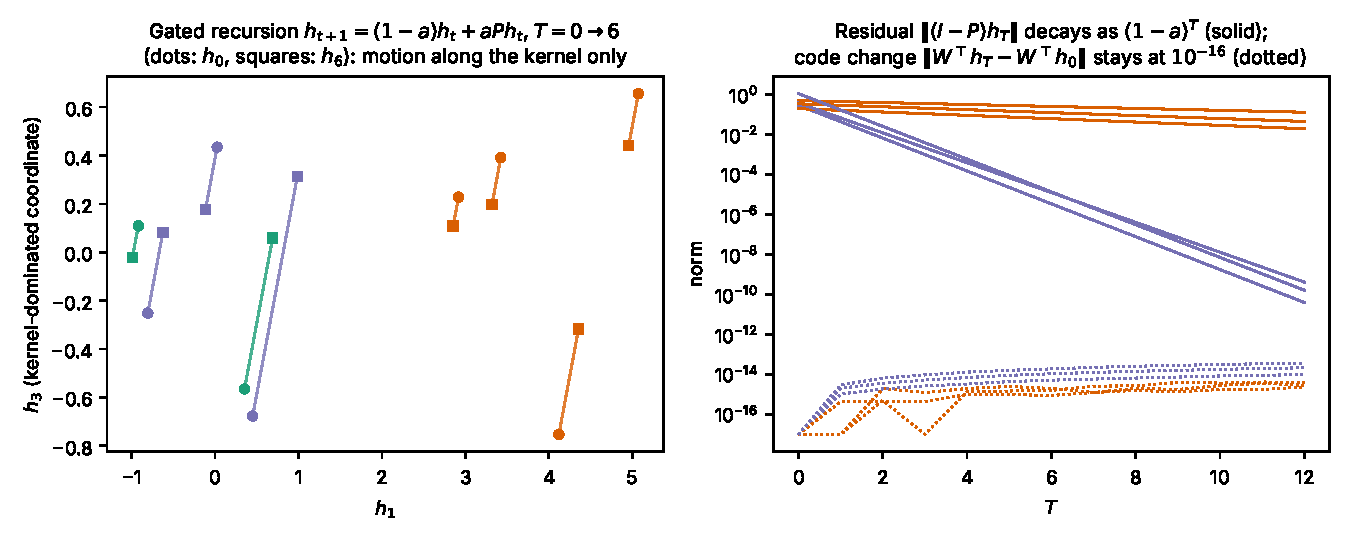
\includegraphics[width=\textwidth]{fig_recursion.pdf}
\caption{Proposition~\ref{prop:code} on the worked example of
Section~\ref{sec:worked}. Left: trajectories $h_0\to h_6$ of nine test points
under the gated recursion, plotted in the coordinates $(h_1,h_3)$; all
segments are parallel, since the motion is confined to the one-dimensional
kernel. Right: the residual norm decays geometrically with a point-dependent
rate $1-a(x)$ (solid), while the change of the code stays at machine
precision (dotted) for every $T$.}
\label{fig:recursion}
\end{figure}
\paragraph{Consequences.} (a) A read-out connected to the code $c=W^\T h_T$
sees \emph{exactly the same thing} for every $T$. (b) With the analytic
gate, $T$ only sets how strongly the residual is damped: $(1-a(x))^T\to0$
for every $x$, faster where $a(x)$ is large, which pushes $h_T$ towards $Px$
and hurts a read-out on $h_T$ in small samples (conditioning,
Section~\ref{sec:small}). (c) For this block, a dependence of the gate on $t$
requires a gate reading outside $\spn(W)$: a design choice, not an automatic
property of the non-linearity. (d) The answer to the parameter-saving
question is therefore two-sided: shared-weight recursion does save a factor
$L$ ($\mathcal O(Ldr)\to\mathcal O(dr)$), but with this gate the $T$ steps
are equal to a \emph{single} step with the gate $a_T(x)=1-(1-a(x))^T$
(equation~\eqref{eq:gate-collapse}). The number of steps therefore changes
the function computed on the residual, through a scalar that depends on the
code only; it gives the non-linearity access to no new coordinate of the
input, and it does not change a read-out on the code at all.

\subsection{An exact Jacobian determinant for the gated block}
For the linear stack, $\det\mathcal T\neq0$ is the Liouville--Jacobi
guarantee against representational collapse; with a non-linearity the
guarantee is usually only local. For the gated oblique block the
determinant is available in closed form.

\begin{theorem}[Exact determinant of the gated oblique block]
\label{thm:gate-det}
Let $P=UW^\T$ be idempotent of rank $r$ and
$F(h)=h+\tfrac{a(h)}{L}(P-I)h$, $a(h)=\sigma(s^\T h+b)\in(0,1)$, $L\ge1$. Then
\begin{equation}
  \det\nabla F(h)=\Bigl(1-\tfrac aL\Bigr)^{d-r}\Bigl(1-\frac{a(1-a)}{L-a}\,s^\T(I-P)h\Bigr)
  =\Bigl(1-\tfrac aL\Bigr)^{d-r-1}\Bigl(1-\tfrac aL-\tfrac{a(1-a)}{L}\,s^\T(I-P)h\Bigr).
  \label{eq:det-gate}
\end{equation}
In particular, for $L=1$, $\det\nabla F=(1-a)^{d-r}(1-a\,s^\T(I-P)h)$, and $F$
is a local diffeomorphism at $h$ if and only if $a\,s^\T(I-P)h\neq1$.
\end{theorem}
\begin{proof}
$\nabla F=B+\tfrac1L(P-I)h\,(\nabla a)^\T$ with $B=(1-\tfrac aL)I+\tfrac aLP$
and $\nabla a=a(1-a)s$. $B$ has eigenvalue $1$ on $\im P$ and $1-\tfrac aL$ on
$\ker P$. Since $(P-I)h\in\ker P$, $B^{-1}(P-I)h=(P-I)h/(1-\tfrac aL)$, and
the matrix determinant lemma~\cite{hornjohnson2013} gives
$\det\nabla F=\det B\,(1+\tfrac1L(\nabla a)^\T B^{-1}(P-I)h)
=(1-\tfrac aL)^{d-r}(1-\tfrac{a(1-a)}{L-a}s^\T(I-P)h)$.
\end{proof}
Verified by central finite-difference Jacobians ($d=12$, $r=3$): agreement
to the eight digits displayed for general $s$ ($-5.1138954\times10^{-3}$ for
$L=1$, $5.2176658\times10^{-2}$ for $L=2$); $\det=(1-a)^{d-r}=0.76077713$
when $s\in\spn(W)$; $|\det|<10^{-14}$ on a case constructed with
$a\,s^\T(I-P)h=1$. The theorem quantifies the trade-off left qualitative by
Proposition~\ref{prop:code}: for the gate to vary along the orbit it must
read the residual ($s^\T(I-P)h\neq0$), but for $L=1$ it must not read it
\emph{too much} ($a\,s^\T(I-P)h<1$) if the orientation is to be preserved.
The residual normalisation $1/L$ relaxes the condition
($|s^\T(I-P)h|<L/a$ suffices for a positive determinant), and suggests a
possible regulariser, $\max(0,\,a\,s^\T(I-P)h-1+\epsilon)$, which is not
tested here.

\begin{example}[Theorems~\ref{thm:collapse} and~\ref{thm:gate-det} in dimension three]
\label{ex:det}
Take $d=3$, $r=1$, $u=(1,0,0)$, $w=(1,1,0)$, so $w^\T u=1$, $P=uw^\T$ maps $h$
to $(h_1+h_2,0,0)$, $\ker P=\{h:\ h_1+h_2=0\}=\spn\{(-1,1,0),e_3\}$ and
$(I-P)h=(-h_2,h_2,h_3)$. Gate $s=(0,0,1)$, $b=0$: it reads $h_3$, entirely in
the kernel ($s^\T(I-P)h=h_3$). At $h=(1,\tfrac12,2)$, $a=\sigma(2)=0.8808$.
\begin{itemize}
  \item $L=1$: $\det\nabla F=(1-a)^2(1-2a)=0.0142\times(-0.7616)=-0.010822$
  (finite differences: $-0.010822$). The determinant is \emph{negative}: at
  $h_3=2$ the gate has already crossed the threshold $\sigma(h_3)h_3=1$,
  reached at $h_3^\ast=1.2785$ (numerical determinant $2.4\times10^{-11}$);
  the block reverses orientation and is not injective near the plane
  $h_3=h_3^\ast$ (its third coordinate, $h_3(1-\sigma(h_3))$, has a maximum
  there).
  \item $L=2$: $\det\nabla F=(1-\tfrac a2)^2(1-\tfrac{a(1-a)}{2-a}\cdot2)=0.3132\times0.8124=+0.254399$
  (finite differences: $+0.254399$). For this value of $a$ the determinant
  would vanish only at $s^\T(I-P)h=(L-a)/(a(1-a))=10.66$, and the sufficient
  condition $|s^\T(I-P)h|<L/a=2.27$ is met. In fact, since $a=\sigma(h_3)$
  here and $\sup_xx\,\sigma'(x)=0.224<1\le L-a$, the second factor
  of~\eqref{eq:det-gate} stays above $0.80$ for every $h_3$: with $L=2$ the
  determinant of this block never vanishes.
\end{itemize}
The same projector illustrates Theorem~\ref{thm:collapse}:
$(I+P/2)^2-I=1.25P$ and $(I+P/2)^3-I=2.375P$ exactly; on $h=(1,\tfrac12,2)$
two linear steps give $(2.875,\tfrac12,2)=h+1.25\,(1.5,0,0)$: only the code
coordinate $h_1+h_2=1.5$ has been touched, and only by a constant factor.
\end{example}

\subsection{Reduction of gated depth to \texorpdfstring{$r+m$}{r+m} coordinates}
\label{sec:thmA}
Consider the block gated per code coordinate (the triceptron of
Section~\ref{sec:tri} in residual form, i.e.\ $h+Ph/L$ with an
input-dependent rank mask),
\begin{equation}
  F(h)=h+\tfrac1L\,U\,\diag\bigl(a(h)\bigr)W^\T h,\qquad
  a(h)=\sigma(S^\T h+b)\in(0,1)^r,\quad S\in\R^{d\times r},
  \label{eq:blocA}
\end{equation}
and its shared-weight iterates $h_{t+1}=F(h_t)$, $h_T=F^{(T)}(h_0)$.

\begin{theorem}[Reduction of gated depth]
\label{thm:A}
Let $A=S^\T U\in\R^{r\times r}$ and $\beta=S^\T(I-P)h_0\in\R^r$.
\begin{enumerate}
  \item[(i)] \textbf{Invariant residual}: $(I-P)h_t=(I-P)h_0$ for all $t$.
  \item[(ii)] \textbf{Code recursion in dimension $r$}:
  $c_{t+1}=c_t\odot\bigl(1+\tfrac1L\sigma(Ac_t+\beta+b)\bigr)$.
  \item[(iii)] \textbf{Structure in $T$}: $h_T=U\Phi_T(c_0,\beta)+(I-P)h_0$,
  where $\Phi_T$ is the $T$-fold iterate of
  $\varphi_\beta(c)=c\odot(1+\sigma(Ac+\beta+b)/L)$; the code $c_T=W^\T h_T$
  depends on the input only through the $2r$ numbers
  $(W^\T h_0,\,S^\T(I-P)h_0)$, and the residual $(I-P)h_0$ is carried
  unchanged.
  \item[(iv)] \textbf{Read-out}: for every linear read-out
  $h\mapsto V_{\mathrm{ro}}h+v_0$,
  $V_{\mathrm{ro}}h_T+v_0=V_{\mathrm{ro}}U\,\Phi_T(W^\T h,\,S^\T(I-P)h)+V_{\mathrm{ro}}(I-P)h+v_0$:
  the non-linearity acts on $r+m$ linear functionals of the input only, with
  $m=\rank(S^\T(I-P))\le r$, whatever $T$.
  \item[(v)] \textbf{Case $\im S\subset\spn(W)$}: $\beta=0$, $\Phi_T(c,0)$ is a
  fixed reparametrisation of the code and the kernel $\ker W^\T$ enters the
  output only linearly, for every $T$ (this generalises
  Proposition~\ref{prop:code}(ii)).
  \item[(vi)] \textbf{Scalar variant} $F(h)=h+\tfrac{a(h)}{L}(P-I)h$,
  $a=\sigma(s^\T h+b)$: the code is invariant and
  $(I-P)h_T=\Lambda_T(c_0,\,s^\T(I-P)h_0)\,(I-P)h_0$ with $\Lambda_T$ scalar:
  the \emph{direction} of the residual is fixed and the kernel enters through
  a single functional, whatever $s$. For $s\notin\spn(W)$ no closed form in
  $T$ is given, but the recursion is a scalar one.
\end{enumerate}
\end{theorem}
\begin{proof}
(i) $(I-P)U=U-UW^\T U=0$, so $(I-P)F(h)=(I-P)h$.
(ii) $W^\T F(h)=c+\tfrac1LW^\T U\diag(a)W^\T h=c+\tfrac1La\odot c$, and
$S^\T h=S^\T Uc+S^\T\rho=Ac+\beta$ with $\rho$ constant by (i).
(iii)--(v) follow: $h_T=Uc_T+\rho_0$ with $c_T=\Phi_T(c_0,\beta)$; if $S=WB$
then $S^\T(I-P)=B^\T W^\T(I-P)=B^\T(W^\T-W^\T UW^\T)=0$.
(vi) $W^\T(P-I)=0$ gives code invariance; $(I-P)(P-I)h=-(I-P)h$ gives
$(I-P)F(h)=(1-a/L)(I-P)h$, and $a(h_t)=\sigma(s^\T Uc_0+\lambda_ts^\T\rho_0+b)$
with $\lambda_{t+1}=\lambda_t(1-a_t/L)$, $\lambda_0=1$.
\end{proof}

\begin{proposition}[Exact determinant of the block~\eqref{eq:blocA}]
\label{prop:detA}
$\det\nabla F(h)=\det\bigl(I_r+\tfrac1L[\diag(a)+\diag(c\odot a\odot(1-a))A]\bigr)$,
an $r\times r$ determinant.
\end{proposition}
\begin{proof}
$\nabla F=I_d+UM$ with $M=\tfrac1L[\diag(a)W^\T+\diag(c\odot a\odot(1-a))S^\T]$;
$\det(I_d+UM)=\det(I_r+MU)$ (Sylvester) and
$MU=\tfrac1L[\diag(a)+\diag(c\odot a\odot(1-a))A]$.
\end{proof}
Verified by finite differences ($d=10$, $r=3$, $L=2$, three random points):
$-3.33654787$, $5.35252229$ and $1.54207626$, in agreement to at least seven
significant digits. A sufficient condition for a non-zero determinant is
strict row diagonal dominance of this $r\times r$ matrix, which holds as soon
as $|c_i|\,a_i(1-a_i)\,\|A_{i\cdot}\|_1<L+a_i$ for every $i$.

\begin{corollary}[Depth acts on at most $r+m$ coordinates]
\label{cor:A1}
The set of functions realisable by $T$ shared steps of the
block~\eqref{eq:blocA} followed by a linear read-out is contained in
$\{h\mapsto g(W^\T h,\,S^\T(I-P)h)+\ell(h)\}$ with $g:\R^{r+m}\to\R^C$ and
$\ell$ linear. Two inputs with the same code and the same $m$ residual
functionals are separated only linearly, for every $T$. The number of steps
changes $g$ within the family of iterates of $\varphi_\beta$; it does not
increase the number $r+m$ of coordinates on which the non-linearity acts.
\end{corollary}
\begin{remark}[What the reduction does and does not say]
\label{rem:depth}
Theorem~\ref{thm:A} and Corollary~\ref{cor:A1} are statements about the
\emph{arguments} of the non-linearity, not about its \emph{form}:
\emph{depth does not enlarge the subspace of information accessible to the
non-linearity; it can nevertheless modify the function computed on that
subspace}. The function $g_T=V_{\mathrm{ro}}U\,\Phi_T$ is a $T$-fold
iterate, and iterates of a fixed map can be markedly more complex functions
of their $r+m$ arguments than the map itself (Example~\ref{ex:A3} gives
numbers). Whether this additional complexity is useful on a given problem
is an empirical question that the theorem leaves open. What the theorem
excludes is that additional steps make the non-linearity sensitive to
directions of the input that the code and the $m$ gate functionals do not
contain: such directions enter the output linearly at every $T$.
\end{remark}

\begin{corollary}[Rank one: under a monotonicity condition, depth does not change the topology of the boundary]
\label{cor:A2}
For $r=1$, $\varphi_\beta(c)=c(1+\sigma(\alpha c+\beta+b)/L)$ with
$\alpha=s^\T u$, and $\varphi_\beta'(c)>1$ when $\alpha c\ge0$,
$\varphi_\beta'(c)\ge1-|\alpha c|/(4L)$ when $\alpha c<0$. Let $I$ be an
interval of initial codes such that $\alpha c_t>-4L$ for $t=0,\dots,T-1$
along every orbit starting in $I$, for the values of $\beta$ considered
(this holds automatically where $\alpha c_0\ge0$, and it is implied,
uniformly in $\beta$, by $|\alpha c_0|(1+1/L)^{T-1}<4L$). Then
$\Phi_T(\cdot,\beta)$ is strictly increasing on $I$ for these $\beta$, so
every linear threshold on $\Phi_T$ defines, within $I$, a region
$\{c>\psi_T(\beta)\}$ (or $\{c<\psi_T(\beta)\}$) for a single function
$\psi_T$, possibly equal to an endpoint of $I$ (empty or full region):
depth deforms one boundary curve (a graph over $\beta$) and does not create
a second one.
\end{corollary}
\begin{proof}
$\varphi_\beta'=1+\sigma/L+c\alpha\sigma'/L$ with $\sigma>0$ and
$0<\sigma'\le1/4$. Since $c_{t+1}=c_t(1+\sigma/L)$, the sign of $c_t$ is
constant and $|c_t|\le|c_0|(1+1/L)^t$. By the chain rule,
$\partial c_T/\partial c_0=\prod_{t<T}\varphi_\beta'(c_t)>0$ under the stated
condition, and the threshold $v\,\Phi_T(c,\beta)>\theta$ inverts to
$c>\psi_T(\beta)$ if $v>0$ and to $c<\psi_T(\beta)$ if $v<0$.
\end{proof}
The condition cannot simply be dropped: for $L=1$, $\alpha=1$, $b=0$ and
$\beta=12$, $\varphi_\beta(-16)=-16.29$, $\varphi_\beta(-12)=-18.00$ and
$\varphi_\beta(-8)=-15.86$, so that $\{\varphi_\beta>-17\}$ has two
components after a single step. The constant $4L$ is sufficient, not sharp:
since $\varphi_\beta'=1+\sigma/L+\alpha c\,\sigma(1-\sigma)/L$ and
$\inf_{\sigma\in(0,1)}\frac{L+\sigma}{\sigma(1-\sigma)}=2L+1+2\sqrt{L(L+1)}$
(attained at $\sigma=\sqrt{L(L+1)}-L$), $\varphi_\beta'(c)>0$ for every
$\beta$ if and only if $\alpha c>-(2L+1+2\sqrt{L(L+1)})$, i.e.\ $-5.83$,
$-9.90$, $-17.94$ for $L=1,2,4$ (confirmed numerically).

\paragraph{Numerical verification} ($d=12$, $r=3$, $L=4$, $T=6$). Invariant
residual to $2.3\times10^{-16}$; code recursion in dimension $r$ to
$4.6\times10^{-16}$; two inputs with the same $(c_0,S^\T\rho_0)$ whose
residuals differ by $3.0$ in norm give the same $c_T$ to $1.7\times10^{-14}$;
with $\im S\subset\spn(W)$, $c_T$ ignores the residual to
$2.7\times10^{-15}$; at rank one ($\alpha=0.4$, $c_0\in[-3,3]$, so that the
condition of Corollary~\ref{cor:A2} holds), $c_0\mapsto c_T$ is strictly
increasing; for the scalar variant, $\cos\angle(\rho_T,\rho_0)=1$ to
$10^{-12}$.

\begin{example}[The gate reads the kernel: two different inputs, one code]
\label{ex:A1}
Same geometry as Example~\ref{ex:det}, $L=2$, $T=3$, $b=0$: code
$c=h_1+h_2$, residual $(-h_2,h_2,h_3)$. Gate $s=(0,0,1)$: $s^\T(I-P)=(0,0,1)\ne0$,
so $m=1$, and $A=s^\T u=0$. By Theorem~\ref{thm:A}(ii), $a_t=\sigma(\beta)$
with $\beta=h_3$ independent of $t$, so the recursion solves in closed form,
$c_T=c_0(1+\sigma(h_3)/L)^T$. For $h=(1,\tfrac12,2)$ and $h'=(0.2,1.3,2)$,
same code $c_0=1.5$ and same $\beta=2$ but different residuals,
$(-0.5,0.5,2)$ and $(-1.3,1.3,2)$. Three steps give
$h_T=(3.9827,0.5,2)$ and $h_T'=(3.1827,1.3,2)$: different vectors, the
\emph{same code} $c_T=4.4827$, and the closed form returns
$1.5\,(1+0.8808/2)^3=4.4827$. The residuals are unchanged. Any linear
read-out separates $h$ from $h'$ only through the linear term
$V_{\mathrm{ro}}(I-P)h_0$, whatever $T$: Corollary~\ref{cor:A1} in dimension three. The
determinant of Proposition~\ref{prop:detA} is a scalar here, $A=0$, so
$\det\nabla F=1+a/L=1.4404$, recovered by finite differences. With
$s=w=(1,1,0)$ instead ($s\in\spn(W)$, $m=0$), the inputs $(1,\tfrac12,2)$ and
$(1,\tfrac12,-7)$ give the same $c_T=4.5151$: the kernel is ignored by the
non-linearity (Theorem~\ref{thm:A}(v)).
\end{example}

\begin{example}[Rank one with $A\ne0$: a single boundary curve]
\label{ex:A2}
Same geometry, $L=2$, gate $s=(1,0,1)$: $A=s^\T u=1$ and
$\beta=s^\T(I-P)h=h_3-h_2$. No closed form is known for the recursion
$c\leftarrow c(1+\sigma(c+\beta)/L)$, but it is strictly increasing in $c_0$
on the range used below (Corollary~\ref{cor:A2}: positive codes satisfy the
condition trivially, and the negative orbits stay above $-2.93>-4L=-8$).
At $\beta=0.5$: $c_0=-2,-1,0,1,2$ give $c_1=-2.1824,-1.1888,0,1.4088,2.9241$
and $c_6=-2.9261,-2.1664,0,9.8550,21.9073$. Depth amplifies positive codes
and leaves $c=0$ fixed; the order is preserved. The threshold $c_T>1$ inverts
to $c_0>\psi_T(\beta)$, computed by bisection: $\psi_1(\beta)=0.8897,0.7467,0.6812$
and $\psi_6(\beta)=0.5425,0.2055,0.1055$ for $\beta=-2,0,2$. Going from
$T=1$ to $T=6$ shifts and tilts the curve in the $(c,\beta)$ plane; it does
not create a second component.
\end{example}

\begin{example}[Rank two: it is $m$, not $T$, that counts]
\label{ex:A3}
$d=4$, $U=[e_1,e_2]$, $W=[e_1+e_3,e_2+e_4]$ ($W^\T U=I_2$); $Ph=(h_1+h_3,h_2+h_4,0,0)$
and $(I-P)h=(-h_3,-h_4,h_3,h_4)$. Two inputs with the same code $(1.3,1.3)$
and the same $h_3$: $h=(1,0.5,0.3,0.8)$ and $h'=(1,3.3,0.3,-2)$, differing in
$h_4$ (and in $h_2$ to compensate the code). With $L=2$, $T=4$:
if both gates read $h_3$ ($S=[e_3,e_3]$, $m=1$) then
$c_T(h)=c_T(h')=(3.5691,3.5691)$: four steps have not distinguished $h$ from
$h'$, because they differ in a kernel direction the gate does not read. If
the gates read $h_3$ and $h_4$ ($S=[e_3,e_4]$, $m=2$) then
$c_T(h)=(3.5691,4.2542)$ and $c_T(h')=(3.5691,1.6388)$: the second coordinate
now separates them. With $m=1$, additional steps do not separate $h$ from
$h'$ through the non-linearity: $c_T(h)=c_T(h')$ at $T=4$, $8$ and $40$,
as Theorem~\ref{thm:A}(iv) requires, since the two inputs share their
$r+m=3$ functionals. Additional steps do change the function computed on
those functionals: for a third input $h''=(2,0.5,-1,0.8)$, with code
$(1.0,1.3)$ and $h_3=-1$, the ratio of the first code coordinates
$c_T(h)_1/c_T(h'')_1$ is $1.3$ at $T=0$ and $2.1547$, $3.5713$ and
$203.39$ at $T=4$, $8$ and $40$. Sensitivity to a new direction of the
input is thus bought with independent gate directions in the kernel
($m$), whereas the number of steps ($T$) reshapes the response to the
directions already read.
\end{example}

\paragraph{Design rule.} For the two gate families analysed above, the
non-linearity of a shared block built on a \emph{single} projector has at
most $r+m$ linear functionals of the input as arguments, whatever the
number of steps (for the scalar variant it multiplies the residual by a
scalar); the function of these arguments does depend on the number of
steps (Remark~\ref{rem:depth}). Within this reduction, independent gate directions in the kernel
raise $m$ up to $r$ (the triceptron, Section~\ref{sec:tri}); outside it,
several non-aligned projectors with a non-linearity between them (the
lattice, Appendix~\ref{sec:lattice}) are one route, not claimed to be the
only one.

%% =====================================================================
\section{Capacity of multiplicative units: the triceptron}
\label{sec:tri}
%% =====================================================================
A perceptron has one direction ($w$); the oblique perceptron has two ($u$ for
representation, $w$ for measurement). The \emph{triceptron} has three: a
\emph{gate} direction $s$ that is free to differ from $w$,
\begin{equation}
  y=\sigma(s^\T x+b_s)\cdot\frac{w^\T x}{w^\T u}\ \ (\text{rank one}),\qquad
  h=\sigma(S^\T x+b_s)\odot(W^\T x+b_w),\ \ \text{output }V_{\mathrm{ro}}h\ \ (\text{rank }r).
  \label{eq:tri}
\end{equation}
The motivation comes from Proposition~\ref{prop:code}: in the recursion of
the oblique block, a gate that reads inside $\spn(W)$ is constant along the
orbit and brings nothing that the code does not already contain; a gate
direction outside $\spn(W)$ reads the residual. (With $s=w$ the unit is
still a genuine non-linearity of $x$: it is the SiLU unit,
Theorem~\ref{thm:B}(i).) At rank $r$ the unit is a gated linear
unit~\cite{dauphin2017glu}: $W$ is the ``up'' projection, $S$ the gate,
$V_{\mathrm{ro}}$ the ``down'' projection of the SwiGLU feed-forward blocks~\cite{shazeer2020glu}
used in recent language models. The gate$\times$code product makes each unit
a \emph{quadratic} function of $x$ to second order in the gate
pre-activation, where a ReLU unit is piecewise linear.

\subsection{Quadric capacity of the triceptron}
Unit: $\tau(x)=\sigma(\gamma(s^\T x+b_s))\,(w^\T x+b_w)$, with a gate
sharpness $\gamma>0$ (a notational convenience: it can be absorbed in $s$
and $b_s$); layer: $f(x)=\sum_{i=1}^kv_i\tau_i(x)+u^\T x+u_0$ (the linear
term $u^\T x$ is a \emph{skip}; the experiments of
Section~\ref{sec:tri-exp} are run with and without it). The \emph{inertia} $(p,n)$ of a real symmetric
matrix is its number of positive and of negative eigenvalues.
\begin{theorem}[Capacity of the triceptron]
\label{thm:B}
\begin{enumerate}
  \item[(i)] \textbf{Inclusion.} For $s_i=w_i$, $b_{s,i}=b_{w,i}=b_i$ and
  $\gamma=1$, $\tau_i=\mathrm{SiLU}(w_i^\T x+b_i)$: every one-hidden-layer
  SiLU (swish) network with $k$ units is a network of $k$ triceptrons. For
  general $\gamma$,
  $\sup_z|\sigma(\gamma z)z-\mathrm{ReLU}(z)|=c_0/\gamma$ with
  $c_0=\max_{t>0}t/(1+e^t)\approx0.2785$: every one-hidden-layer ReLU network
  with $k$ units is the uniform limit, as $\gamma\to\infty$, of networks of
  $k$ triceptrons. Decoupling $s$ from $w$ is, for the activation, what
  obliquity is for the linear layer.
  \item[(ii)] \textbf{Soft regime: quadrics.} As $\gamma\to0$, with read-out
  weights $v_i/\gamma$ and a skip chosen to cancel the linear terms (its
  coefficients are of order $1/\gamma$), $f$ converges, uniformly on every
  compact set and with an error $O(\gamma^2)$, to a polynomial of degree two
  whose quadratic part has matrix
  $Q=\tfrac18\sum_iv_i(s_iw_i^\T+w_is_i^\T)$. Conversely, every real
  symmetric matrix of inertia $(p,n)$ can be written in this way with
  $k=\max(p,n)$ units, and not with fewer. Hence, on any compact set, $k$
  soft triceptrons plus a skip approximate to $O(\gamma^2)$ every quadratic
  function whose quadratic part satisfies $\max(p,n)\le k$; where the
  gradient of that function does not vanish on its zero set, the decision
  boundary converges to the quadric (in Hausdorff distance, on compact sets)
  at the same rate. Special cases: the
  XOR pattern $\mathrm{sign}(x_1x_2)$ (inertia $(1,1)$): one unit, exact in
  sign for every $\gamma$; an ellipsoid of $\R^d$ (inertia $(d,0)$): $d$
  units; a hyperbola: one unit.
  \item[(iii)] \textbf{Hard regime: the cell count of a ReLU layer.} As
  $\gamma\to\infty$ the layer tends, pointwise away from the gate
  hyperplanes, to a function that is affine on each cell of the arrangement
  of the $k$ gate hyperplanes, of which there are at
  most $\sum_{j\le d}\binom kj$ (Zaslavsky~\cite{zaslavsky1975}); the value
  hyperplanes $w_i$ create no cells. This is the bound that holds for a
  $k$-unit ReLU layer; the difference is that the affine piece of each cell
  combines the $w_i$ freely instead of being tied to the gate directions.
  \item[(iv)] \textbf{A necessary width for ReLU on a curved boundary.} Let
  $\mathcal D\subset\R^2$ be the open region assigned to one class by a
  one-hidden-layer ReLU network with $m$ units and an affine read-out (with
  or without a linear skip), and call it $\varepsilon$-accurate for the disc
  of radius $R$ if $B(0,R-\varepsilon)\subset\mathcal D\subset\bar B(0,R+\varepsilon)$,
  $0<\varepsilon<R$. The boundary $\partial\mathcal D$ is contained in at
  most $N(m)=1+m+\binom m2$ segments or half-lines, and in at most $2m$
  segments if $\mathcal D$ is convex and bounded. A region whose boundary is
  contained in $N$ segments or half-lines is $\varepsilon$-accurate only if
  \begin{equation}
    N\ \ge\ \frac{\pi}{\arccos\frac{R-\varepsilon}{R+\varepsilon}},
    \qquad\text{i.e.}\qquad
    \varepsilon\ \ge\ R\tan^2\frac{\pi}{2N}\ \sim\ \frac{\pi^2R}{4N^2},
    \label{eq:polygon}
  \end{equation}
  with equality, for $N\ge3$, for the regular $N$-gon of apothem
  $R-\varepsilon$ and circumradius $R+\varepsilon$. Hence no such network is
  exact, and
  $\varepsilon$-accuracy requires $m\gtrsim(\pi^2R/\varepsilon)^{1/4}$ units
  in general and $m\ge\tfrac\pi4\sqrt{R/\varepsilon}\,(1+o(1))$ units when
  $\mathcal D$ is convex. These are necessary conditions; whether a network
  can actually place $N(m)$ segments around a circle is not established
  here, and the convex case suggests that it cannot. By contrast, the two
  soft triceptrons of (ii) with a skip are $\varepsilon$-accurate with
  $\varepsilon=\gamma^2R^3/24+O(\gamma^4)$ at fixed width two, at the price
  of read-out and skip weights of order $1/\gamma$.
\end{enumerate}
\end{theorem}
\begin{proof}
(i) With $t=-\gamma z$ for $z<0$, $|\sigma(\gamma z)z|=\gamma^{-1}t/(1+e^t)$,
and for $z>0$, $|\sigma(\gamma z)z-z|=\gamma^{-1}t/(1+e^t)$ with
$t=\gamma z$; the maximum of $t/(1+e^t)$ over $t>0$ is $c_0$. The uniform
convergence of the network follows from
$|\sum_iv_i(\tau_i-\mathrm{ReLU}_i)|\le c_0\sum_i|v_i|/\gamma$.
(ii) $\sigma(\gamma z)=\tfrac12+\tfrac{\gamma z}4+O(\gamma^3z^3)$, so
$\tau_i=\tfrac12(w_i^\T x+b_{w,i})+\tfrac\gamma4(s_i^\T x+b_{s,i})(w_i^\T x+b_{w,i})+O(\gamma^3)$
uniformly on compact sets; the skip absorbs the linear terms and the
read-out $v_i/\gamma$ isolates the quadratic term, of symmetric matrix
$\tfrac18\sum v_i(s_iw_i^\T+w_is_i^\T)$, with a remainder $O(\gamma^2)$.
Each $\mathrm{sym}(sw^\T)=\tfrac12(sw^\T+ws^\T)$ has inertia $(1,1)$ if $s,w$
are independent (its non-zero eigenvalues are
$\tfrac12(s^\T w\pm\|s\|\|w\|)$), and $(1,0)$ or $(0,1)$ if they are
collinear. Conversely, write the spectral decomposition
$Q=\sum_{j\le p}\lambda_je_je_j^\T-\sum_{j\le n}\nu_jf_jf_j^\T$ with
$\lambda_j,\nu_j>0$ and orthonormal $e_j,f_j$; for $j\le\min(p,n)$,
$\lambda_je_je_j^\T-\nu_jf_jf_j^\T=\mathrm{sym}\bigl((\sqrt{\lambda_j}e_j+\sqrt{\nu_j}f_j)(\sqrt{\lambda_j}e_j-\sqrt{\nu_j}f_j)^\T\bigr)$,
and the remaining $|p-n|$ terms are collinear units. Hence $\max(p,n)$ units
suffice. They are necessary because the numbers of positive and of negative
eigenvalues are subadditive under addition of symmetric matrices (a
consequence of Weyl's inequalities~\cite{hornjohnson2013}) and each unit
contributes at most one eigenvalue of each sign. For XOR,
$\sigma(\gamma x_1)x_2-\tfrac12x_2=\tfrac12x_2\tanh(\gamma x_1/2)$ has the
sign of $x_1x_2$ for every $\gamma>0$.
(iii) In the limit $\tau_i$ is affine on each open half-space of its gate
hyperplane; the layer is affine on each cell of the arrangement of the $k$
gate hyperplanes, whose number of cells in $\R^d$ is at most
$\sum_{j=0}^d\binom kj$.
(iv) The network function $f$ is continuous and affine on each closed cell
of the arrangement of the $m$ kink lines, and $\mathcal D=\{f<\theta\}$ (or
$\{f>\theta\}$). A point of $\partial\mathcal D$ satisfies $f=\theta$ and is
a limit of points of $\mathcal D$ lying in one closed cell on which
$f-\theta$ is not identically zero; it therefore belongs to the zero line of
the affine piece of that cell: at most one segment or half-line per cell,
and at most $N(m)$ cells. If $\mathcal D$ is convex, $\partial\mathcal D$ is a convex
polygon whose vertices lie on kink lines, and a line contains at most two
vertices of a convex polygon: at most $2m$ edges. If $\mathcal D$ is
$\varepsilon$-accurate, $\partial\mathcal D$ lies in the closed annulus
$R-\varepsilon\le\|x\|\le R+\varepsilon$, and every ray from the origin
meets $\partial\mathcal D$ (it starts in $\mathcal D$ and leaves it). The
part of a segment or half-line lying in that annulus is seen from the origin
under a total angle of at most $2\arccos\frac{R-\varepsilon}{R+\varepsilon}$:
if its supporting line is at distance $h\ge R-\varepsilon$ from the origin
the angle is at most $2\arccos\frac{h}{R+\varepsilon}$; if $h<R-\varepsilon$
that part consists of at most two pieces, one on each side of the foot of
the perpendicular, each seen under at most
$\arccos\frac{h}{R+\varepsilon}-\arccos\frac{h}{R-\varepsilon}\le\arccos\frac{R-\varepsilon}{R+\varepsilon}$,
this difference being increasing in $h$. $N$ such angles must cover $2\pi$,
which is~\eqref{eq:polygon} since
$\cos\frac\pi N\ge\frac{R-\varepsilon}{R+\varepsilon}$ is equivalent to
$\varepsilon\ge R\tan^2\frac\pi{2N}$. For the two triceptrons,
$\sum_i\tfrac{x_i}2\tanh\tfrac{\gamma x_i}2=\tfrac\gamma4\|x\|^2-\tfrac{\gamma^3}{48}(x_1^4+x_2^4)+O(\gamma^5)$,
whose level set at $\tfrac\gamma4R^2$ has polar radius
$R+\tfrac{\gamma^2R^3}{24}(\cos^4\theta+\sin^4\theta)+O(\gamma^4)$.
\end{proof}

\paragraph{Numerical verification.} (i) $\sup_z|\sigma(\gamma z)z-\mathrm{ReLU}(z)|=5.569\times10^{-3}$
at $\gamma=50$, equal to $0.2785/\gamma$. (ii) Circle with two soft units
and a skip: the largest radial gap between the level set and the unit circle
is $1.05\times10^{-2}$, $1.67\times10^{-3}$ and $1.04\times10^{-4}$ for
$\gamma=0.5$, $0.2$ and $0.05$, i.e.\ $\gamma^2/24$; XOR with one unit plus
skip, and with two hard units ($\gamma=50$, $x_2\tanh(25x_1)$): $100\%$ sign
agreement off the axes on a $301\times301$ grid. (iv) Disc \emph{without
margin} (class $=\|x\|>1$, $4000$ training points uniform in
$[-1.5,1.5]^2$): ReLU MLPs with $m$ units trained by L-BFGS (three
initialisations, the one with the best \emph{training} accuracy is kept) are
evaluated on a $601\times601$ grid of the same square, by the fraction of
misclassified area and by the accuracy $\hat\varepsilon$ in the sense of
(iv), estimated as the largest $|\,\|x\|-1|$ over misclassified grid points:
\begin{center}
\small
\begin{tabular}{@{}rrrrrr@{}}
\toprule
$m$ & $N(m)$ & misclassified area & measured $\hat\varepsilon$ & bound $\tan^2\frac{\pi}{2N(m)}$ & convex bound $\tan^2\frac{\pi}{4m}$ \\
\midrule
2 & 4 & $32.08\%$ & 1.121 & 0.1716 & 0.1716 \\
3 & 7 & $2.76\%$ & 0.136 & 0.0521 & 0.0718 \\
4 & 11 & $1.55\%$ & 0.070 & 0.0207 & 0.0396 \\
6 & 22 & $1.09\%$ & 0.070 & 0.0051 & 0.0173 \\
10 & 56 & $0.75\%$ & 0.050 & $7.9\times10^{-4}$ & 0.0062 \\
20 & 211 & $0.51\%$ & 0.027 & $5.5\times10^{-5}$ & 0.0015 \\
40 & 821 & $0.35\%$ & 0.024 & $3.7\times10^{-6}$ & $3.9\times10^{-4}$ \\
\bottomrule
\end{tabular}
\end{center}
The measured accuracies are above the general bound, as they must be, and
also above the convex bound (which is binding only for convex regions); they
decrease much more slowly than either: the trained networks are far from
the best polygon with the same number of units, so that the bounds say
nothing about what optimisation achieves in practice. ($\hat\varepsilon$ is
itself a lower estimate, computed on a grid of the training square; at
$m=2$ it exceeds $R$, i.e.\ that network is not $\varepsilon$-accurate for
any admissible $\varepsilon$.) The two soft triceptrons with explicit
weights ($\gamma=0.05$) misclassify $0.014\%$ of the grid, with a radial gap
of $1.04\times10^{-4}$. With a margin (\texttt{make\_circles}, factor $0.5$),
three ReLU units reach $100\%$ training accuracy (two units: $83.3\%$): it is
the margin, not the curvature, that sets the unit requirement; the
capacity advantage of the triceptron concerns tight curved boundaries, and
Section~\ref{sec:tri-exp} measures how much of it is visible in trained
models.

\begin{example}[The inclusion in numbers]
With $s=w$ and $z=w^\T x+b=2$: $\gamma=1$ gives $\sigma(2)\cdot2=1.7616=\mathrm{SiLU}(2)$;
$\gamma=50$ gives $\sigma(100)\cdot2=2.0000$ and, at $z=-2$,
$\sigma(-100)\cdot(-2)=-7\times10^{-44}$, i.e.\ $\mathrm{ReLU}(\pm2)$ to
machine precision. The largest gap, $0.2785/\gamma=5.6\times10^{-3}$, is
reached near $z=\pm1.28/\gamma$. A ReLU neuron is the $\gamma\to\infty$ limit
of a triceptron whose gate direction is \emph{aligned} with its value
direction.
\end{example}

\begin{example}[XOR with one unit and a skip]
Take $s=e_1$, $w=e_2$, $b_s=b_w=0$, $\gamma=0.05$, read-out $v=1$ and skip
$u=-\tfrac12e_2$: $f(x)=\sigma(0.05x_1)x_2-\tfrac12x_2=0.0125\,x_1x_2+O(10^{-4})$
on $[-2,2]^2$. The skip cancels the linear term $\tfrac12x_2$ of the
expansion of $\sigma$; only the cross term remains, with matrix
$Q=\tfrac\gamma8(e_1e_2^\T+e_2e_1^\T)$, inertia $(1,1)$: a rectangular
hyperbola whose asymptotes are the axes, i.e.\ the XOR pattern. At
$(\pm1,\pm1)$: $f=\pm0.01250$ with the sign of $x_1x_2$ in all four cases; at
$(\pm2,0.5)$: $\pm0.01249$ against $\pm0.01250$. With the same skip, a single
ReLU unit can separate the four canonical XOR points ($|x_1+x_2|-1$ does),
but not the pattern $\mathrm{sign}(x_1x_2)$ on the whole plane:
$v\,\mathrm{ReLU}(\cdot)$ plus an affine function is convex or concave, so
one of its two decision regions is convex, whereas neither $\{x_1x_2>0\}$
nor $\{x_1x_2<0\}$ is. One triceptron
realises it because gate and value look in orthogonal directions. The small
values ($10^{-2}$) are only a matter of scale: the read-out $v/\gamma$ of the
theorem brings them back to $x_1x_2/4$.
\end{example}

\begin{example}[The unit circle with two units]
Units $(s_1,w_1)=(e_1,e_1)$ and $(s_2,w_2)=(e_2,e_2)$, $\gamma=0.05$, skip
$-\tfrac12(x_1+x_2)$: $f(x)=\sum_i[\sigma(0.05x_i)x_i-\tfrac12x_i]=0.0125(x_1^2+x_2^2)+O(\gamma^3)$,
inertia $(2,0)$; decide ``outside'' if $f>0.0125R^2$ with $R=1$. Then
$f(0.9,0)=0.01012$ (inside), $f(1.1,0)=0.01512$ (outside),
$f(0.7,0.7)=0.01225$ (inside, $\|x\|^2=0.98$), $f(0.6,0.9)=0.01462$ (outside,
$\|x\|^2=1.17$), $f(-0.5,0.5)=0.00625$ (inside): all correct. The point
$(0.7,0.7)$, at $0.02$ of the circle in squared norm, is classified
correctly: the boundary is a smooth closed curve within
$\gamma^2/24\approx10^{-4}$ of the unit circle, not a polygon.
\end{example}

\begin{figure}[t]
\centering
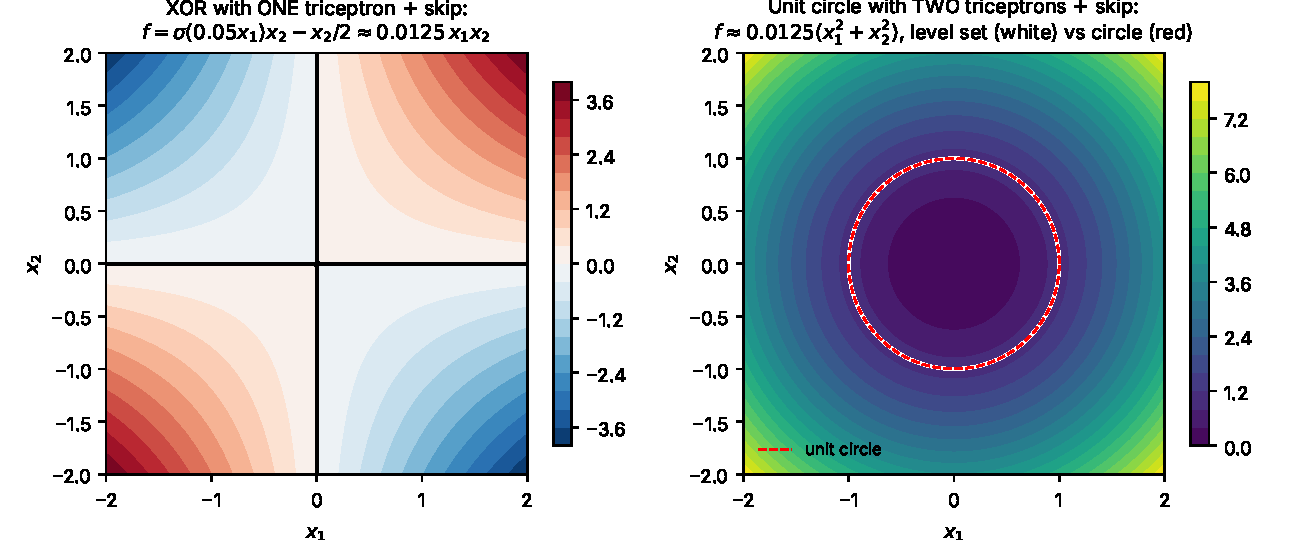
\includegraphics[width=0.95\textwidth]{fig_triceptron.pdf}
\caption{The two soft-regime constructions of Theorem~\ref{thm:B}(ii) as
functions of the plane (values divided by $\gamma/4=0.0125$). Left: one
triceptron plus a linear skip realises the saddle $x_1x_2$ to second order,
i.e.\ the XOR pattern, with the axes as zero set. Right: two triceptrons plus
a skip realise $x_1^2+x_2^2$ to second order; the level set at $0.0125$
(white) is indistinguishable at this scale from the unit circle (red dashed;
the radial gap is $10^{-4}$), a boundary that a ReLU layer approaches only by
increasing its width.}
\label{fig:tri}
\end{figure}
\begin{example}[Reading the inertia on $\mathrm{sym}(sw^\T)$]
Hyperbola $x_1^2-x_2^2$: one unit, $s=(1,1)$, $w=(1,-1)$:
$\tfrac12(sw^\T+ws^\T)=\diag(1,-1)$, eigenvalues $\tfrac12(0\pm2)=\pm1$,
inertia $(1,1)$. Ellipse $2x_1^2+x_2^2$: inertia $(2,0)$, two collinear
units $s=w=(\sqrt2,0)$ and $s=w=(0,1)$, whose sum is $\diag(2,1)$; in the
soft limit one unit cannot make an ellipse, since $\mathrm{sym}(sw^\T)$ has
at most one positive eigenvalue. Saddle $x_1^2+x_2^2-x_3^2$ in $\R^3$:
inertia $(2,1)$, so two units: $s=(1,0,1)$, $w=(1,0,-1)$ (contributing
$x_1^2-x_3^2$) and $s=w=e_2$ (contributing $x_2^2$); the sum is
$\diag(1,1,-1)$. This is the construction of the proof of (ii): one positive
and one negative eigenvalue are paired per unit, the $|p-n|$ remaining ones
go into collinear units.
\end{example}

\begin{example}[The necessary width in numbers]
For the disc $R=1$, a ReLU layer with $m=2,3,4,6,10,20$ units has at most
$N(m)=4,7,11,22,56,211$ boundary segments, hence by~\eqref{eq:polygon} an
accuracy $\varepsilon\ge0.1716,\,0.0521,\,0.0207,\,0.0051,\,7.9\times10^{-4},\,5.5\times10^{-5}$.
Conversely, an accuracy $\varepsilon=10^{-2},10^{-3},10^{-4}$ needs
$N\ge16,50,158$ segments, i.e.\ at least $m=5,10,18$ ReLU units ($N(5)=16$,
$N(10)=56$, $N(18)=172$), and at least $8,25,79$ units if the decision
region is convex. Two soft triceptrons reach these accuracies at fixed
width, with $\gamma\le0.48,\,0.15,\,0.048$. The growth in
$\varepsilon^{-1/4}$ is a necessary condition, independent of the optimiser;
it is not claimed to be attainable.
\end{example}

\begin{example}[Hard regime: a switch]
$s=e_1$, $w=e_2$, $\gamma=50$: $\tau(x)=\sigma(50x_1)x_2$ equals $3.0000$ at
$(1,3)$ and $0.0000$ at $(-1,3)$: it is close to $\mathbf 1[x_1>0]\,x_2$,
one variable \emph{switching} another, which is what a gated linear unit
does. The transition has width $\sim1/\gamma$: $1.8674$ at $(0.01,3)$,
$1.1326$ at $(-0.01,3)$. A ReLU layer realises this switch approximately on
bounded sets, as $\mathrm{ReLU}(x_2+Mx_1)-\mathrm{ReLU}(Mx_1)$ with large
$M$, with two units; in both cases a large weight ($M$ or $\gamma$) sets the
width of the transition, and the difference is that the triceptron has the
product inside a single unit.
\end{example}

\begin{remark}[Squared-norm units]
A unit of the form $\|P_{U,W}x\|^2=x^\T P^\T Px$ is a positive
semi-definite quadratic form of rank $r$: thresholded alone, it bounds a
convex (cylindrical) set. Signed combinations of several such units can
realise indefinite forms, so the difference with the triceptron is one of
economy per unit: a single triceptron already brings inertia $(1,1)$, an
indefinite (hyperbolic) quadric.
\end{remark}

\subsection{Experiments aligned with the theorem}
\label{sec:tri-exp}
Theorem~\ref{thm:B} is a statement about what a layer \emph{with a linear
skip} can represent, with explicit weights in a soft regime. An experiment
can only be said to illustrate it if it (a)~compares gated and ReLU layers
under the same optimiser, (b)~includes the skip, and (c)~separates the
weights constructed in the proof from the weights found by training. The
three points are treated in turn. Comparing a hand-trained gated layer
with a library-trained MLP would confound the architecture with the
optimiser (last column of Table~\ref{tab:tri}), and is avoided.

\paragraph{Models and trainer.} \emph{GLU}: the layer~\eqref{eq:tri} with
$r$ units, parameters $(W,b_w,S,b_s,V_{\mathrm{ro}},b_0)$, i.e.\
$2dr+2r+rC+C$ parameters. \emph{MLP}: one hidden ReLU layer whose width $h$
gives the nearest number of parameters. Both exist with and without a
linear skip $Kx$ added to the output ($dC$ additional parameters). All four
models are trained by the \emph{same} code: full-batch Adam, $2000$ steps,
learning rate $10^{-2}$, $L_2$ penalty $10^{-4}$, the same initialisation
scale, hand-written gradients verified by finite differences (relative
errors between $7.6\times10^{-8}$ and $1.9\times10^{-7}$ for the four
models). The two-dimensional problems (two moons with noise $0.15$,
concentric circles with radius ratio $0.5$ and noise $0.1$, XOR pattern
$\mathrm{sign}(x_1x_2)$ on Gaussian inputs; $n=400$, $70/30$ split) are
drawn independently ten times; differences are paired by draw and reported
with the conventions of Section~\ref{sec:central}.
\begin{table}[h]
\centering\small\renewcommand{\arraystretch}{1.1}
\caption{Gated (GLU, $r$ units) against ReLU (MLP, $h$ units) layers at nearly equal parameter counts, same trainer, without and with a linear skip. Test accuracy in \% (mean $\pm$ standard deviation over 10 independent draws) and paired difference GLU $-$ MLP in points with its 95\% interval ($\approx$ equivalent within one point, $\uparrow$ GLU better, $\downarrow$ GLU worse, ? undetermined). Last column: the MLP without skip trained by scikit-learn's L-BFGS, a different optimiser, for reference only.}
\label{tab:tri}
\resizebox{\textwidth}{!}{\begin{tabular}{@{}llrrrrrrrrr@{}}
\toprule
 & & \multicolumn{4}{c}{without skip} & \multicolumn{4}{c}{with linear skip} & \\
\cmidrule(lr){3-6}\cmidrule(lr){7-10}
problem & $r/h$ & param. & GLU & MLP & GLU $-$ MLP & param. & GLU & MLP & GLU $-$ MLP & MLP, L-BFGS \\
\midrule
two moons & $16/26$ & $130/132$ & $98.8\pm0.9$ & $98.9\pm0.9$ & $-0.1\,[-0.4,+0.3]^{\approx}$ & $134/136$ & $98.8\pm1.1$ & $98.9\pm0.9$ & $-0.2\,[-0.4,+0.1]^{\approx}$ & $98.5\pm0.9$ \\
two moons & $4/6$ & $34/32$ & $98.7\pm0.9$ & $98.9\pm0.9$ & $-0.2\,[-0.5,+0.0]^{\approx}$ & $38/36$ & $98.8\pm0.8$ & $98.8\pm1.1$ & $+0.1\,[-0.4,+0.5]^{\approx}$ & $96.8\pm2.8$ \\
two moons & $2/3$ & $18/17$ & $97.6\pm3.8$ & $91.0\pm4.0$ & $+6.6\,[+2.8,+10.4]^{\uparrow}$ & $22/21$ & $98.8\pm0.9$ & $95.6\pm4.9$ & $+3.2\,[-0.6,+6.9]^{?}$ & $89.5\pm4.0$ \\
two moons & $1/2$ & $10/12$ & $88.2\pm2.2$ & $88.8\pm2.7$ & $-0.7\,[-1.5,+0.1]^{?}$ & $14/16$ & $94.6\pm5.4$ & $91.2\pm4.4$ & $+3.4\,[-2.9,+9.7]^{?}$ & $84.8\pm12.0$ \\
\addlinespace
circles & $16/26$ & $130/132$ & $99.1\pm0.7$ & $99.2\pm0.7$ & $-0.2\,[-0.4,+0.1]^{\approx}$ & $134/136$ & $99.1\pm0.7$ & $99.2\pm0.6$ & $-0.1\,[-0.3,+0.1]^{\approx}$ & $99.2\pm0.7$ \\
circles & $4/6$ & $34/32$ & $99.0\pm0.8$ & $98.8\pm0.9$ & $+0.2\,[-0.1,+0.4]^{\approx}$ & $38/36$ & $99.0\pm0.8$ & $98.8\pm0.8$ & $+0.2\,[-0.1,+0.4]^{\approx}$ & $97.9\pm1.8$ \\
circles & $2/3$ & $18/17$ & $98.3\pm1.5$ & $92.5\pm10.7$ & $+5.8\,[-2.1,+13.7]^{?}$ & $22/21$ & $98.6\pm1.4$ & $98.0\pm2.1$ & $+0.6\,[-0.4,+1.6]^{?}$ & $82.9\pm11.2$ \\
circles & $1/2$ & $10/12$ & $70.6\pm3.9$ & $69.7\pm6.9$ & $+0.9\,[-5.1,+6.9]^{?}$ & $14/16$ & $70.5\pm3.9$ & $81.9\pm13.9$ & $-11.4\,[-22.0,-0.8]^{\downarrow}$ & $72.2\pm4.2$ \\
\addlinespace
XOR & $16/26$ & $130/132$ & $97.9\pm1.6$ & $99.0\pm0.7$ & $-1.1\,[-2.3,+0.2]^{?}$ & $134/136$ & $98.8\pm0.8$ & $99.2\pm0.6$ & $-0.5\,[-1.4,+0.4]^{?}$ & $98.3\pm1.6$ \\
XOR & $4/6$ & $34/32$ & $98.2\pm1.1$ & $98.3\pm1.2$ & $-0.0\,[-0.6,+0.6]^{\approx}$ & $38/36$ & $98.1\pm1.3$ & $98.7\pm0.9$ & $-0.6\,[-1.8,+0.6]^{?}$ & $98.4\pm0.9$ \\
XOR & $2/3$ & $18/17$ & $98.4\pm1.3$ & $88.3\pm10.9$ & $+10.1\,[+1.8,+18.4]^{\uparrow}$ & $22/21$ & $98.0\pm1.2$ & $95.5\pm8.3$ & $+2.5\,[-3.9,+8.9]^{?}$ & $83.0\pm12.6$ \\
XOR & $1/2$ & $10/12$ & $74.2\pm4.6$ & $70.7\pm7.1$ & $+3.4\,[-3.1,+10.0]^{?}$ & $14/16$ & $98.7\pm0.8$ & $90.3\pm11.6$ & $+8.3\,[-0.7,+17.3]^{?}$ & $70.8\pm6.7$ \\
\bottomrule
\end{tabular}}
\end{table}

\paragraph{(a) Same trainer: parity, except at about eighteen parameters
without skip.} From $32$ parameters upwards the two families are equivalent
within one point or undetermined on the three problems, with or without
skip. At $18$ against $17$ parameters without
skip (two gated units against three ReLU units) the gated layer is ahead on
two moons ($+6.6$ points, interval $[+2.8,+10.4]$) and on XOR ($+10.1$,
$[+1.8,+18.4]$); on circles the difference ($+5.8$) is undetermined, the
ReLU layer having a standard deviation of $10.7$ points over the draws.
With the skip the three differences at this size ($+3.2$, $+0.6$, $+2.5$)
are undetermined. The last column shows why the optimiser must be shared:
at $17$ parameters the library L-BFGS training of the same MLP is $1.5$ to
$9.6$ points below the Adam training used here, so that a comparison
across optimisers would attribute to the architecture a gap that belongs
largely to the optimisation.

\paragraph{(b) The widths of Theorem~\ref{thm:B}(ii) are observed, and the
skip plays the role the proof gives it.} The XOR pattern is a quadric of
inertia $(1,1)$: the theorem asks for $\max(p,n)=1$ unit and a skip that
cancels the linear term. One gated unit with skip ($14$ parameters) reaches
$98.7\pm0.8\%$; the same unit without skip reaches $74.2\%$. The circle
has inertia $(2,0)$ and asks for two units: one gated unit reaches
$70.6\%$ without and $70.5\%$ with skip, two units $98.3\%$ and $98.6\%$.
The comparison with ReLU layers at these sizes is not one-sided. On XOR,
two ReLU units with skip ($16$ parameters) reach $90.3\pm11.6\%$, and the
difference to the gated unit ($+8.3$ points) is undetermined. On circles,
two ReLU units with skip reach $81.9\pm13.9\%$ and are \emph{ahead} of the
single gated unit ($-11.4$ points, interval $[-22.0,-0.8]$): a single
gated unit cannot produce a definite quadratic form in the soft regime,
whatever its parameters, whereas two ReLU units already bound a strip.

\paragraph{(c) Constructed against learned weights.} The weights of the
proof, used without any training on the raw data, give
\begin{center}\small
\begin{tabular}{@{}lrrrr@{}}
\toprule
gate sharpness $\gamma$ & $1$ & $0.5$ & $0.2$ & $0.05$ \\
\midrule
circles, two units $+$ skip, accuracy (\%) & $99.7$ & $99.7$ & $99.6$ & $99.6$ \\
XOR, one unit $+$ skip, accuracy (\%) & $100.0$ & $100.0$ & $100.0$ & $100.0$ \\
largest weight in normalised form ($4/\gamma$) & $4$ & $8$ & $20$ & $80$ \\
\bottomrule
\end{tabular}
\end{center}
(accuracy on the $400$ points of each of the ten draws; the circles are
noisy, so that $100\%$ is not attainable). The soft regime
$\gamma\to0$ is needed for the \emph{approximation} statement of the
theorem (the radial gap is $\gamma^2R^3/24$), not for classification: on
these data $\gamma=1$, with weights of order $4$, is as accurate as
$\gamma=0.05$, whose read-out weights are of order $80$. The weights
\emph{learned} by Adam for the same two architectures reach $98.8\pm1.1\%$
(circles) and $98.6\pm0.8\%$ (XOR) on the test sets, with a largest weight
of about $7.7$ and gate directions of norm $3.7$ and $7.5$ (standardised
inputs): training finds solutions with moderately sharp gates, not the
soft-regime construction. The theorem therefore accounts for the
\emph{widths} at which the two problems become solvable, which is what the
experiments reproduce; it does not describe the solutions reached by
gradient descent, and it says nothing of the parity observed at larger
widths, where both families have enough units.

\paragraph{Larger problems, and the analytic realisation.} Two further
realisations are compared on eight datasets with $r=16$ (five $70/30$
splits of a fixed dataset; the intervals measure split variability only).
\emph{TRI-CF} uses analytic features: $(U,W)$ from the fast block, $S$ the
$k$ leading principal components of the residual $(I-P)x$ (outside
$\spn(W)$ by construction), features $[c,\ c_ia_j]$, a least-squares
read-out, $k$ chosen by internal cross-validation.
\begin{table}[h]
\centering\small\renewcommand{\arraystretch}{1.1}
\caption{Width $r=16$: analytic block (centroid read-out), TRI-CF (least-squares read-out on its features; with $k=0$ it reduces to the block with the least-squares read-out), and the gated and ReLU layers of Table~\ref{tab:tri} without skip (same trainer). Test accuracy in \%, 5 splits of a fixed dataset. Parameters: GLU / MLP.}
\label{tab:tri-all}
\resizebox{\textwidth}{!}{\begin{tabular}{@{}lrrrrrrr@{}}
\toprule
dataset & param. & analytic block & TRI-CF & GLU & MLP & GLU $-$ MLP & MLP, L-BFGS \\
\midrule
two moons & $130/132$ & $86.8\pm3.2$ & $86.8\pm3.2$ ($k{=}2$) & $98.2\pm1.3$ & $98.0\pm1.1$ & $+0.2\,[-0.3,+0.6]^{\approx}$ & $96.7\pm1.9$ \\
circles & $130/132$ & $46.0\pm4.1$ & $69.5\pm6.4$ ($k{=}2$) & $99.8\pm0.3$ & $100.0\pm0.0$ & $-0.2\,[-0.6,+0.3]^{\approx}$ & $99.3\pm0.3$ \\
XOR & $130/132$ & $50.0\pm0.9$ & $80.2\pm6.2$ ($k{=}2$) & $98.0\pm0.8$ & $97.8\pm0.7$ & $+0.2\,[-1.2,+1.5]^{?}$ & $96.3\pm1.5$ \\
Gaussian $n{=}15$/cl ($d{=}20$) & $740/729$ & $96.7\pm4.4$ & $93.3\pm6.5$ ($k{=}0$) & $90.0\pm5.4$ & $90.0\pm5.4$ & $+0.0\,[+0.0,+0.0]^{\approx}$ & $90.0\pm5.4$ \\
heteroscedastic $n{=}60$/cl & $740/729$ & $93.6\pm1.1$ & $92.2\pm1.7$ ($k{=}2$) & $93.3\pm1.0$ & $92.8\pm1.4$ & $+0.6\,[-0.4,+1.5]^{?}$ & $91.9\pm1.6$ \\
digits & $2154/2170$ & $95.3\pm0.2$ & $94.6\pm0.3$ ($k{=}7$) & $98.0\pm0.6$ & $98.0\pm0.4$ & $-0.0\,[-0.3,+0.3]^{\approx}$ & $96.4\pm0.8$ \\
breast & $1026/1025$ & $95.4\pm0.9$ & $95.6\pm0.9$ ($k{=}4$) & $96.4\pm0.9$ & $96.6\pm0.7$ & $-0.2\,[-0.9,+0.4]^{\approx}$ & $96.0\pm1.2$ \\
wine & $499/496$ & $100.0\pm0.0$ & $99.3\pm0.9$ ($k{=}1$) & $98.9\pm0.9$ & $99.3\pm0.9$ & $-0.4\,[-1.4,+0.7]^{?}$ & $99.6\pm0.7$ \\
\bottomrule
\end{tabular}}
\end{table}
On the eight datasets the gated and ReLU layers are equivalent or
undetermined (differences between $-0.4$ and $+0.6$ point): at a
comfortable budget the triceptron is \emph{different}, not better. On the
small Gaussian sample the three gradient-trained models give the same
accuracy on every split ($90.0\%$, on $18$ test points per split) and stay
behind the analytic block ($96.7\%$), with about $740$ parameters for
$42$ training samples. The analytic version of the gate is not enough:
gate directions taken from the residual help (XOR $50\to80\%$, circles
$46\to70\%$) but remain far from a \emph{learned} gate ($98$ to $100\%$).
This is one of the two places in this report where a gradient-trained
component was clearly better than every back-propagation-free construction
tried (the learned lifting of Appendix~\ref{sec:fourier} is the other):
$s$ is not a second-order statistic of the classes (for XOR the class
means coincide in population and the Fisher block is blind).

\paragraph{What is established.} Gated linear
units~\cite{dauphin2017glu,shazeer2020glu} and multiplicative (sigma--pi)
units~\cite{rumelhart1986} are known; what is added here is the geometric
reading (a third direction, the gate, decoupled from the measurement
direction), the capacity statements of Theorem~\ref{thm:B}, and
measurements under a common trainer. These measurements support a narrow
conclusion: the widths predicted for the two quadrics are the widths at
which a gated layer with skip solves them; an accuracy advantage over ReLU
layers was observed only at about eighteen parameters without skip, on two
problems out of three; and no advantage is observed from thirty-two
parameters upwards or on the higher-dimensional datasets.

\subsection{Summary of the two capacity results}
What the two theorems of this section and of Section~\ref{sec:thmA} say:
Theorem~\ref{thm:A} settles, for the two gate families analysed, the
question of shared-weight depth of a single oblique block (the
non-linearity acts on at most $r+m$ linear functionals, whatever $T$); for
these blocks, recursion alone does not give the non-linearity access to
new directions of the input, and sensitivity to such directions has to come
from gate directions that read the kernel or from non-aligned projectors. Theorem~\ref{thm:B} situates the
triceptron: it contains SiLU networks and has ReLU networks as uniform
limits; it approximates quadrics to any accuracy at fixed width
$\max(p,n)$; and it has the cell-count bound of ReLU in the hard regime.
The experiments reproduce the minimal widths of (ii) and show an accuracy
gap to ReLU layers only at about eighteen parameters without skip; they do
not show an advantage at larger widths. Neither theorem depends on how the
weights are obtained: they are statements about the \emph{architecture}.

%% =====================================================================
\section{An analytic discriminant block}
\label{sec:block}
%% =====================================================================

\subsection{From Fisher's rank-one direction to a rank-\texorpdfstring{$r$}{r} projector}
For two classes, the Fisher-optimal oblique perceptron~\cite{fisher1936} has
representation direction $u=\mu_1-\mu_0$ and measurement direction $w^\ast=S_W^{-1}u$: a
result in closed form. The multi-class, multi-rank generalisation is the Fisher
generalised eigenvalue problem (GEVP)
\begin{equation}
  S_B\,v_i=\lambda_i\,S_W\,v_i,\qquad \lambda_1\ge\lambda_2\ge\cdots,
  \label{eq:gevp}
\end{equation}
solved by a standard dense symmetric eigensolver
(\texttt{scipy.linalg.eigh(S\_B, S\_W)}), with no gradient-based
optimisation. The generalised eigenvectors are the
\emph{measurement} directions (at rank one and for two classes,
$v_1\propto S_W^{-1}(\mu_1-\mu_0)=w^\ast$), and the representation directions
follow:
\begin{equation}
  W_{\mathrm{raw}}=[v_1,\dots,v_r],\qquad
  U_{\mathrm{raw}}=S_W\,W_{\mathrm{raw}}=\bigl[S_Bv_i/\lambda_i\bigr]_i\subset\spn(\mu_c-\bar\mu),
  \label{eq:uw}
\end{equation}
the inclusion coming from $S_Wv_i=S_Bv_i/\lambda_i\in\im S_B$. The oblique
code $c=(W^\T U)^{-1}W^\T h$ is then exactly the vector of Fisher
discriminant scores, the sufficient statistic of linear discriminant analysis
(LDA); Proposition~\ref{prop:lda} states the equivalence precisely.

\begin{remark}[A convention that is easy to get wrong]
Setting $U=[v_i]$ and $W=S_W^{-1}U$ instead shifts both matrices by a power of
$S_W^{-1}$ relative to the natural convention ($u$ in the space of means,
$w=S_W^{-1}u$). The code is then $V^\T S_W^{-1}x$, which is \emph{not} the
vector of Fisher scores $V^\T x$: the resulting classifier is no longer LDA.
The geometric readings (angles to the true subspaces, Kronecker and kernel
variants) and the optimality statements of this report hold for
convention~\eqref{eq:uw}, which is that of the $M$-orthogonal projector
$P=U(U^\T MU)^{-1}U^\T M$ with $M=S_W^{-1}$.
\end{remark}

When $S_W$ is noisy ($n$ small relative to $Cd$), it is replaced by its
Ledoit--Wolf shrinkage estimator $S=(1-a)S_W+a\mu I$; Section~\ref{sec:small}
shows that this is necessary well before $n\le d$.

\subsection{Re-whitening: exact idempotence}
Let $V=[v_1,\dots,v_r]$. The Gram matrix
$G=W_{\mathrm{raw}}^\T U_{\mathrm{raw}}=V^\T S_WV$ is symmetric positive
definite, and equals $I_r$ only if the eigenvectors are normalised to be
$S_W$-orthonormal. This is the normalisation returned by
\texttt{scipy.linalg.eigh}, so that in the implementation $G$ differs from
$I_r$ only through the small ridge added to $S_W$ for numerical safety and
through round-off; with any other normalisation, or another solver, $G\ne I_r$.
Re-whitening by its inverse square root,
\begin{equation}
  U\leftarrow U_{\mathrm{raw}}\,G^{-1/2},\qquad W\leftarrow W_{\mathrm{raw}}\,G^{-1/2},
  \label{eq:rewhiten}
\end{equation}
gives $W^\T U=G^{-1/2}GG^{-1/2}=I_r$ exactly, hence $P=UW^\T$ idempotent by
construction, $\kappa(G)=1$ and $\det(I+P/L)=(1+1/L)^r>0$. Measured:
$\|W^\T U-I_r\|$ and $\|P^2-P\|_F$ of the order of $10^{-15}$. (The
factorisation of Section~\ref{sec:fast} makes this step unnecessary: it
produces biorthogonal pairs directly.)

\begin{figure}[t]
\centering
\resizebox{\textwidth}{!}{%
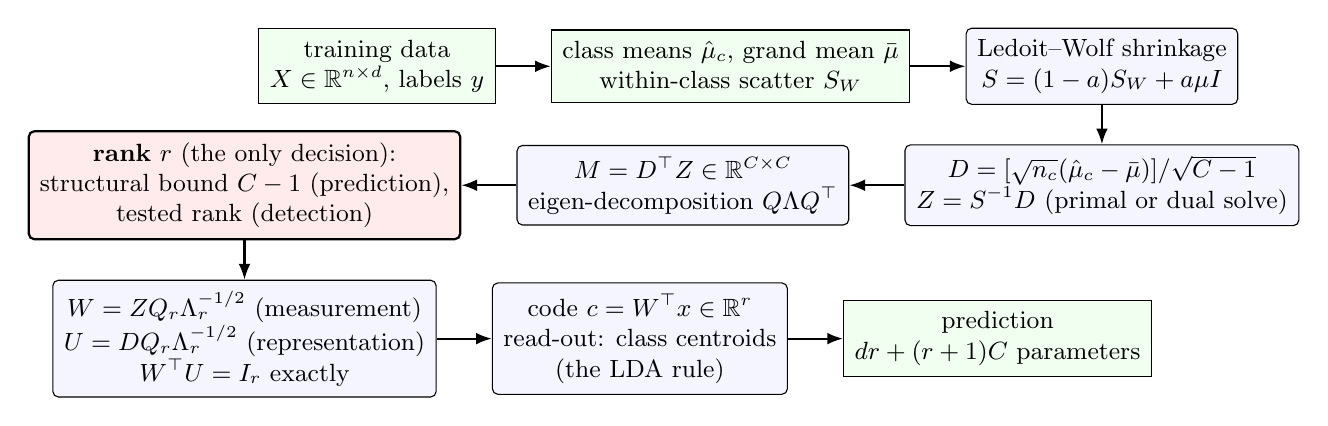
\begin{tikzpicture}[node distance=5mm and 7mm, every node/.style={font=\small},
  box/.style={draw, rounded corners=2pt, align=center, inner sep=4pt, minimum height=9mm, fill=blue!4},
  stat/.style={draw, align=center, inner sep=4pt, minimum height=9mm, fill=green!6},
  dec/.style={draw, rounded corners=2pt, align=center, inner sep=4pt, minimum height=9mm, fill=red!8, thick},
  arr/.style={-{Latex[length=2mm]}, thick}]
  \node[stat] (data) {training data\\$X\in\R^{n\times d}$, labels $y$};
  \node[stat, right=of data] (stats) {class means $\hat\mu_c$, grand mean $\bar\mu$\\within-class scatter $S_W$};
  \node[box, right=of stats] (shr) {Ledoit--Wolf shrinkage\\$S=(1-a)S_W+a\mu I$};
  \node[box, below=of shr] (D) {$D=[\sqrt{n_c}(\hat\mu_c-\bar\mu)]/\sqrt{C-1}$\\$Z=S^{-1}D$ (primal or dual solve)};
  \node[box, left=of D] (M) {$M=D^\T Z\in\R^{C\times C}$\\eigen-decomposition $Q\Lambda Q^\T$};
  \node[dec, left=of M] (rank) {\textbf{rank} $r$ (the only decision):\\structural bound $C-1$ (prediction),\\tested rank (detection)};
  \node[box, below=of rank] (UW) {$W=ZQ_r\Lambda_r^{-1/2}$ (measurement)\\$U=DQ_r\Lambda_r^{-1/2}$ (representation)\\$W^\T U=I_r$ exactly};
  \node[box, right=of UW] (code) {code $c=W^\T x\in\R^r$\\read-out: class centroids\\(the LDA rule)};
  \node[stat, right=of code] (out) {prediction\\$dr+(r+1)C$ parameters};
  \draw[arr] (data) -- (stats); \draw[arr] (stats) -- (shr); \draw[arr] (shr) -- (D); \draw[arr] (D) -- (M);
  \draw[arr] (M) -- (rank); \draw[arr] (rank) -- (UW); \draw[arr] (UW) -- (code); \draw[arr] (code) -- (out);
\end{tikzpicture}}
\caption{The analytic pipeline. Every box is a standard linear-algebra
computation (factorisation, linear solves, one small symmetric
eigen-decomposition); the only decision is the rank
(Section~\ref{sec:rank}). No parameter is learned by gradient or by any
iterative optimisation. The $d\times d$ problem never appears: the
eigen-decomposition is $C\times C$ (Section~\ref{sec:fast}).}
\label{fig:pipeline}
\end{figure}

\subsection{Equivalence with linear discriminant analysis, and the read-out}
\label{sec:lda}
The block is not a new classifier, and the equivalence should be stated
once, exactly.
\begin{proposition}[The block with a centroid read-out is LDA]
\label{prop:lda}
Let $S\succ0$ be the within-class covariance estimate used by the block
(raw or shrunk), $\pi_k=n_k/n$, and let $(U,W)$ be the biorthogonal pair of
rank $r=\rank S_B$ (generically $C-1$), written in the form
$W=S^{-1}DQ_r\Lambda_r^{-1/2}$, $U=SW$ of Proposition~\ref{prop:dual}.
\begin{enumerate}
  \item[(i)] $\spn(W)=S^{-1}\spn\{\mu_k-\bar\mu\}$ and $W^\T SW=I_r$: the
  code $c=W^\T x$ is a whitened coordinate system of the discriminant
  subspace.
  \item[(ii)] For every $x$ and every pair of classes, the LDA log-odds with
  covariance $S$,
  $\delta_k(x)-\delta_l(x)=(\mu_k-\mu_l)^\T S^{-1}\bigl(x-\tfrac12(\mu_k+\mu_l)\bigr)+\log(\pi_k/\pi_l)$,
  is an affine function of the code; conversely every affine function of the
  code is an affine function of the LDA discriminant scores.
  \item[(iii)] The plug-in LDA rule with covariance $S$ is the
  nearest-centroid rule in code space,
  \begin{equation}
    \hat k(x)=\arg\max_k\ -\tfrac12\bigl\|W^\T x-W^\T\mu_k\bigr\|_2^2+\log\pi_k .
    \label{eq:centroid}
  \end{equation}
\end{enumerate}
Hence the block followed by the \emph{centroid read-out}~\eqref{eq:centroid}
makes exactly the predictions of LDA with the covariance estimate $S$; any
other affine read-out of the code (for instance least squares on the class
indicators) is a different classifier built on the same $r$ coordinates.
\end{proposition}
\begin{proof}
(i) The columns of $D$ span $\spn\{\mu_k-\bar\mu\}$, and $Q_r$ spans the
orthogonal complement of $\ker D=\ker(D^\T S^{-1}D)$, so $DQ_r$ and $D$ have
the same column space; $W^\T SW=\Lambda_r^{-1/2}Q_r^\T D^\T S^{-1}DQ_r\Lambda_r^{-1/2}=I_r$.
(ii) $S^{-1}(\mu_k-\mu_l)\in\spn(W)$ by (i), so the log-odds depend on $x$
through $W^\T x$ only, affinely; the $C-1$ independent log-odds and the $r$
code coordinates span the same space of affine functions.
(iii) $P=UW^\T$ is the $S^{-1}$-orthogonal projector onto
$\spn\{\mu_k-\bar\mu\}$, so
$\|x-\mu_k\|_{S^{-1}}^2=\|P(x-\mu_k)\|_{S^{-1}}^2+\|(I-P)(x-\mu_k)\|_{S^{-1}}^2$.
Since $\mu_k-\bar\mu\in\im P$, the second term equals
$\|(I-P)(x-\bar\mu)\|_{S^{-1}}^2$ for every $k$; the first is
$(x-\mu_k)^\T W(U^\T S^{-1}U)W^\T(x-\mu_k)=\|W^\T(x-\mu_k)\|_2^2$ because
$U^\T S^{-1}U=W^\T SW=I_r$.
\end{proof}
Verified on the digits data (ten classes, $n=10$, $30$ and $100$ per class,
ten subsamples each): the predictions of the block with the centroid
read-out coincide with those of an LDA computed directly from the same
shrunk $S$ on $100\%$ of the test points, and with those of scikit-learn's
\texttt{LinearDiscriminantAnalysis(solver="lsqr", shrinkage="auto")} on
$97.1\%$, $98.6\%$ and $99.2\%$ of them. The residual disagreement is one of
covariance estimate, not of classifier: in the implementation used here,
that solver applies the Ledoit--Wolf estimator to each class separately,
after standardising the features within the class, and averages the
resulting class covariances, whereas the block shrinks the pooled
within-class scatter once.

\paragraph{Which read-out.} Two analytic read-outs of the code are used in
this report. The \emph{centroid read-out}~\eqref{eq:centroid} needs no
fitting ($rC$ centroid coordinates and $C$ priors) and is the LDA rule. The
\emph{least-squares read-out} regresses the class indicators on the code
($(r+1)C$ coefficients); it was the read-out of the reference
implementation. The
two are equivalent within one point on the synthetic four-class problems of
Section~\ref{sec:central}, but on the ten-class digits data the
least-squares read-out is $1.7$ to $2.4$ points \emph{below} the centroid
read-out at every sample size, with or without selection (paired $95\%$
intervals excluding zero), the classical masking effect of indicator
regression with many classes~\cite[Section~4.2]{hastie2009}. The ranking is
not universal: on the next-character task of Appendix~\ref{sec:lm}
($35$ classes, one-hot inputs) the least-squares read-out is $3.5$ to $4.6$
points above the centroid rule. The centroid read-out is used as the
reference throughout the report, because it is the LDA rule, which gives
the block a precise statistical meaning, and because it is the better of
the two on the central benchmark. The least-squares read-out is kept only
where it is itself the object of a comparison (the baseline pipeline
diagnosed in Section~\ref{sec:small} and the rows of its ablation, the
paired comparisons of Sections~\ref{sec:central} and~\ref{sec:small}, the
controls of Section~\ref{sec:audit}), and a regression read-out is used
where the features are not the code of a single block (the triceptron
features of Section~\ref{sec:tri-exp}, the concatenated band codes of
Appendix~\ref{sec:fourier}), since the centroid rule has the meaning of
LDA only on the code of one block.

\subsection{An analytic gate}
For the recursion studied in Section~\ref{sec:recursion}, the oblique gate
$y=(1-a(x))x+a(x)Px$, $a(x)=\sigma(s^\T x+b)$, is also fixed in
closed form: $s$ is the first column of $W$ normalised (dominant Fisher
direction) and $b=-s^\T\bar\mu$.

\subsection{The reduced architecture}
\begin{figure}[h]
\centering
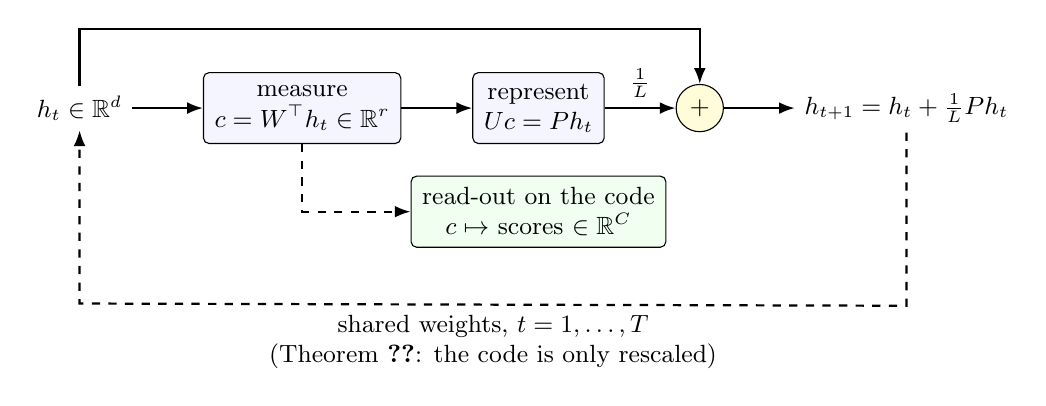
\begin{tikzpicture}[node distance=4mm and 9mm, every node/.style={font=\small},
  box/.style={draw, rounded corners=2pt, align=center, inner sep=4pt, minimum height=9mm, fill=blue!4},
  op/.style={draw, circle, inner sep=1pt, minimum size=6mm, fill=yellow!15},
  arr/.style={-{Latex[length=2mm]}, thick}]
  \node (x) {$h_t\in\R^d$};
  \node[box, right=of x] (W) {measure\\$c=W^\T h_t\in\R^r$};
  \node[box, right=of W] (U) {represent\\$Uc=Ph_t$};
  \node[op, right=of U] (sum) {$+$};
  \node[right=of sum] (hn) {$h_{t+1}=h_t+\tfrac1L Ph_t$};
  \node[box, below=of U, fill=green!6] (ro) {read-out on the code\\$c\mapsto$ scores $\in\R^C$};
  \draw[arr] (x) -- (W); \draw[arr] (W) -- (U); \draw[arr] (U) -- node[above]{$\tfrac1L$} (sum); \draw[arr] (sum) -- (hn);
  \draw[arr] (x) |- ($(sum.north)+(0,7mm)$) -- (sum.north);
  \draw[arr, dashed] (W.south) |- (ro.west);
  \draw[arr, dashed] (hn.south) -- ($(hn.south)+(0,-22mm)$) -- node[below, align=center]{shared weights, $t=1,\dots,T$\\(Theorem~\ref{thm:collapse}: the code is only rescaled)} ($(x.south)+(0,-22mm)$) -- (x.south);
\end{tikzpicture}
\caption{The reduced architecture: one analytic block $(U,W)$ with
$W^\T U=I_r$, optionally applied $T$ times with shared weights, and an
analytic read-out connected to the code $c=W^\T h$, not to the full state.
Because $W^\T P=W^\T$, each pass of the dashed loop multiplies the code by the
constant $1+1/L$ (Theorem~\ref{thm:collapse}), a rescaling that a linear
read-out absorbs; for the gated block of Proposition~\ref{prop:code} the code
does not change at all.}
\label{fig:arch}
\end{figure}
The input is the raw dimension $d$ (no input projection), the output the $C$
classes. Stored parameters, with $r$ the used rank: $dr+(r+1)C$ ($W$, the
$rC$ centroid coordinates and the $C$ constant terms of the centroid
read-out, the same count as a least-squares read-out; $U$ is not needed at
inference when the read-out acts on the code), i.e.\ $76$ for $d=20$,
$r=3$, $C=4$.
Nothing is optimised by gradient.

%% =====================================================================
\section{Exact rank-\texorpdfstring{$(C-1)$}{(C-1)} factorisation of the Fisher problem}
\label{sec:fast}
%% =====================================================================
The analytic block solves \texttt{eigh(S\_B, S\_W)} in dimension $d$: a
Cholesky factorisation of $S_W$ ($d^3/3$), reduction to standard form
($\approx d^3$), and a full diagonalisation ($4$--$9\,d^3$ with vectors). But
$S_B$ has rank at most $C-1$, and this structural property brings everything
down to a problem of size $C$ without any approximation.

\subsection{The equivalent \texorpdfstring{$C\times C$}{CxC} problem}
Write $S_B=DD^\T$ with
$D=[\sqrt{n_c}(\mu_c-\bar\mu)]_c/\sqrt{C-1}\in\R^{d\times C}$.
\begin{proposition}[Dual reduction of the Fisher GEVP]
\label{prop:dual}
Let $S_W\succ0$, $Z=S_W^{-1}D$ and $M=D^\T Z=D^\T S_W^{-1}D\in\R^{C\times C}$
(symmetric positive semi-definite, rank $\le C-1$) with diagonalisation
$M=Q\Lambda Q^\T$. The \emph{non-zero} eigenpairs of $S_Bv=\lambda S_Wv$ are
exactly $(\lambda_i,\,v_i=Zq_i/\sqrt{\lambda_i})$, with $v_i^\T S_Wv_j=\delta_{ij}$.
Moreover, for any $r\le\rank M$, with $Q_r$, $\Lambda_r$ the $r$ leading
eigenvectors and (positive) eigenvalues, and
\begin{equation}
  W=ZQ_r\Lambda_r^{-1/2}\ \ (\text{measurement}),\qquad
  U=DQ_r\Lambda_r^{-1/2}\ \ (\text{representation}),
  \label{eq:uw-fast}
\end{equation}
one has $W^\T U=I_r$ automatically: the re-whitening~\eqref{eq:rewhiten}
becomes unnecessary.
\end{proposition}
\begin{proof}
Let $S_W=RR^\T$ be a Cholesky factorisation and $E=R^{-1}D$. With $z=R^\T v$,
the GEVP $DD^\T v=\lambda RR^\T v$ is the standard problem $EE^\T z=\lambda z$.
The non-zero eigenvalues of $EE^\T$ and of $E^\T E=D^\T R^{-\T}R^{-1}D=M$
coincide with their multiplicities, and if $E^\T Eq=\lambda q$ with
$\lambda>0$ and $\|q\|=1$, then $z=Eq/\sqrt\lambda$ is a unit eigenvector of
$EE^\T$ for $\lambda$ ($\|z\|^2=q^\T E^\T Eq/\lambda=1$), orthonormal
eigenvectors $q_i$ giving orthonormal $z_i$. Hence
$v=R^{-\T}Eq/\sqrt\lambda=S_W^{-1}Dq/\sqrt\lambda=Zq/\sqrt\lambda$ and
$v_i^\T S_Wv_j=z_i^\T z_j=\delta_{ij}$. Finally, with~\eqref{eq:uw-fast}
(for which $U=S_WW$),
$W^\T U=\Lambda_r^{-1/2}Q_r^\T D^\T S_W^{-1}DQ_r\Lambda_r^{-1/2}=I_r$.
\end{proof}
Cost: one factorisation of $S_W$ ($d^3/3$ flops), $C$ solves ($d^2C$), one
$C\times C$ diagonalisation and two $d\times C\times r$ products, instead of
roughly $10d^3$ flops for the full generalised eigen-decomposition. Nothing
is approximated:
$\|P_{\mathrm{fast}}-P_{\mathrm{ref}}\|/\|P_{\mathrm{ref}}\|\le2\times10^{-9}$
and the selected rank is identical (Table~\ref{tab:fast}).

\subsection{Dual form for \texorpdfstring{$n<d$}{n<d}: no \texorpdfstring{$d\times d$}{dxd} matrix}
With Ledoit--Wolf shrinkage, $S=(1-a)X_c^\T X_c/n+a\mu I$, where
$X_c\in\R^{n\times d}$ holds the samples centred by their class means, is a
multiple of the identity plus a matrix of rank at most $n-C$. For $a\mu>0$
the Woodbury identity gives, for any right-hand side $B$,
\begin{equation}
  S^{-1}B=\frac{B}{a\mu}-\frac{(1-a)/n}{a\mu}\,X_c^\T\Bigl(a\mu I_n+\tfrac{1-a}{n}X_cX_c^\T\Bigr)^{-1}X_cB,
  \label{eq:woodbury}
\end{equation}
an $n\times n$ system ($\mathcal O(n^2d+n^3)$) and never a $d\times d$
matrix. The Ledoit--Wolf coefficient itself is computed without $X_c^\T X_c$
through two exact identities: $\|X_c^\T X_c\|_F^2=\|X_cX_c^\T\|_F^2$ (an
$n\times n$ Gram) and $\mathbf 1^\T(X_c^{\circ2})^\T X_c^{\circ2}\mathbf 1=\sum_i\|x_i\|^4$
($\mathcal O(nd)$). Verified: coefficient identical to scikit-learn's to
$10^{-17}$, projector identical to $3.5\times10^{-11}$ ($d=200$,
$n_{\mathrm{train}}=42$). This is the regime of high-dimensional features
computed from a few dozen to a few hundred trials, as in single-subject EEG
classification: at $d=2080$, $n=60$, the fit of the corrected block goes
from $3.9$~s to $2.4$~ms in the run of Table~\ref{tab:fast}.

\subsection{Batched permutation test}
The permutations change $S_B$ but not the metric. Since
$D_p=\bar X^\T Y_pN^{-1/2}/\sqrt{C-1}$ ($\bar X$ globally centred, $Y_p$ the
indicator matrix of the permuted classes), all $n_{\mathrm{perm}}$ matrices
$D_p$ come from \emph{one} product $\bar X^\T[Y_1\cdots Y_{n_{\mathrm{perm}}}]$,
all $S^{-1}D_p$ from \emph{one} solve with $n_{\mathrm{perm}}C$ right-hand
sides, and the maximal eigenvalues from one \texttt{eigvalsh} on a stack of
$C\times C$ matrices. Cost $\mathcal O(n_{\mathrm{perm}}(nd+d^2C))$ instead of
$\mathcal O(n_{\mathrm{perm}}d^3)$, entirely in BLAS-3: $\times116$ at
$d=784$ in the run of Table~\ref{tab:fast}, and $0.2$~s at $d=2080$,
$n=600$, where the reference (about 200 full eigen-decompositions) was not
run. As shown in Section~\ref{sec:rank}, the metric of the batched
test should be the label-free total scatter $S_T$ for the null to be
exchangeable; Table~\ref{tab:fast} times the shared-$S_W$ variant, in order
to compare like with like with the reference implementation, and the $S_T$
variant costs one additional factorisation. The sequential rule of
Section~\ref{sec:rank} reuses the same batch: the deflated statistics are
obtained from the stack of $C\times C$ matrices without any new solve.

\subsection{Further options}
\begin{itemize}
  \item \textbf{Analytic rank (Bartlett/Wilks).} The sequential Bartlett test
  on Wilks' $\Lambda$, $\chi^2=(n-1-\tfrac{d+C}2)\sum_{i>k}\ln(1+\tilde\lambda_i)$
  with $(d-k)(C-1-k)$ degrees of freedom and
  $\tilde\lambda_i=\lambda_i(C-1)/(n-C)$ the eigenvalues on the scale of the
  unnormalised scatter matrices, costs nothing beyond the $\lambda_i$ already
  computed. Its asymptotic calibration is approximate in
  small samples and with shrinkage; it is implemented as an option and
  evaluated in Section~\ref{sec:rank}.
  \item \textbf{Minimal inference.} By Proposition~\ref{prop:code}, a read-out
  on the code depends neither on $T$ nor on the gate: inference reduces to
  $c=W^\T x$ followed by an $r\times C$ map, $\mathcal O(dr)$ per sample, the
  minimum for a rank-$r$ linear classifier.
  \item \textbf{Parallelism.} Everything is BLAS-3; per-subject fits are
  independent; the only sequential part is the $C\times C$ diagonalisation.
  \item \textbf{Online update.} $S_W$ and $D$ are sufficient statistics: a
  new sample updates the Cholesky factor in $\mathcal O(d^2)$ (rank one) and
  replays the $C$ solves, with no GEVP. The rank-one update of the
  within-class scatter is exact: adding $x$ to a class with $n_c$ samples and
  mean $\mu_c$ adds $\tfrac{n_c}{n_c+1}(x-\mu_c)(x-\mu_c)^\T$. Implemented
  (\texttt{OnlineBlock}) and checked ($d=20$, 200 samples then 100 online
  additions): agreement with a batch recomputation at the same frozen
  $(a,\mu,n)$ to $2.6\times10^{-15}$. Two reservations: with the shrinkage
  $(a,\mu)$ and the normalisation $n$ frozen between refits, the projector
  differs from a full refit by $0.8\%$ in relative Frobenius norm in this
  test; and a pure-\texttt{numpy} rank-one Cholesky update (a Python loop)
  does not realise the asymptotic gain ($67$~ms per sample at $d=2080$,
  $n=600$, against $58$~ms for a full fast refit). The $\mathcal O(d^2)$
  versus $\mathcal O(d^3/3)$ gain would require a compiled update, which is
  not provided.
  \item \textbf{What not to do.} A randomised SVD or a Lanczos iteration on
  $S_W^{-1}S_B$ would be approximate and more costly than the exact
  reduction, which exploits the rank-$(C-1)$ structure instead of guessing it.
\end{itemize}

\begin{table}[h]
\centering\small\renewcommand{\arraystretch}{1.12}
\caption{Exactness and timing of the factorisation on a sandbox CPU (corrected block: minimum of 3 runs after warm-up; baseline with 200 permutations: one run after warm-up; the baseline reference at $d=2080$ was not run). ``ref.'': full GEVD \texttt{eigh(S\_B, S\_W)}. Timings vary by a factor of up to two between runs; only the orders of magnitude are meaningful.}
\label{tab:fast}
\resizebox{\textwidth}{!}{\begin{tabular}{@{}rrr|rrr|rrr@{}}
\toprule
$d$ & $n_{\mathrm{train}}$ & $C$ & corrected ref.\ (s) & corrected fast (s) & gain & baseline ref.\ ($+200$ perm.) & baseline fast & gain \\
\midrule
20 & 800 & 4 & 0.002 & 0.0007 & $2\times$ & 0.04 & 0.010 & $4\times$ \\
64 & 1200 & 10 & 0.004 & 0.0016 & $3\times$ & 0.14 & 0.026 & $5\times$ \\
200 & 400 & 4 & 0.016 & 0.0023 & $7\times$ & 0.72 & 0.013 & $55\times$ \\
784 & 1000 & 10 & 0.596 & 0.0437 & $14\times$ & 20.9 & 0.180 & $116\times$ \\
2080 & 60 & 2 & 3.899 & 0.0024 & $1644\times$ & (not run) & 0.022 & --- \\
2080 & 600 & 4 & 4.981 & 0.0468 & $106\times$ & (not run) & 0.202 & --- \\
\midrule
\multicolumn{9}{@{}l}{Exactness ($d=20$): $\|P_{\mathrm{fast}}-P_{\mathrm{ref}}\|/\|P_{\mathrm{ref}}\|=9\times10^{-11}$ (corrected), $2\times10^{-9}$ (baseline); $\|W^\T U-I\|=2\times10^{-15}$ without re-whitening;}\\
\multicolumn{9}{@{}l}{Ledoit--Wolf coefficient identical to scikit-learn ($\le10^{-17}$); identical $r^\ast$; dual $d=200$, $n=42$: $3.5\times10^{-11}$, same accuracy ($100\%$).}\\
\bottomrule
\end{tabular}}
\end{table}
At small $d$ the cost is dominated by Python overheads and the gain is
marginal; it becomes substantial from $d\gtrsim200$ and above all in the
$n<d$ regime, where the dual form avoids every $d\times d$ matrix. The exact reduction also makes the block \emph{simpler}: no
re-whitening, no GEVD, a single primal/dual solver.

\subsection{Against a specialised LDA solver}
\label{sec:fast-lda}
The gains of Table~\ref{tab:fast} are measured against a \emph{dense
generalised eigen-decomposition}, which no careful implementation of LDA
uses. The relevant reference for an LDA estimator is a specialised solver.
Table~\ref{tab:fast-lda} compares the fit of the block (rank $C-1$,
Ledoit--Wolf shrinkage) with scikit-learn's
\texttt{LinearDiscriminantAnalysis}: the \texttt{lsqr} and \texttt{eigen}
solvers with \texttt{shrinkage="auto"}, which estimate the same kind of
model (LDA with a shrunk covariance), and the \texttt{svd} solver, which
has no shrinkage and is therefore a different estimator.
\begin{table}[h]
\centering\small\renewcommand{\arraystretch}{1.12}
\caption{Fit time in seconds (minimum of three runs after warm-up, same data as Table~\ref{tab:fast}) of the block and of scikit-learn's LDA solvers. The \texttt{eigen} solver was not run at $d=2080$. Single CPU, indicative only.}
\label{tab:fast-lda}
\begin{tabular}{@{}rrr|rrrr|r@{}}
\toprule
$d$ & $n_{\mathrm{train}}$ & $C$ & block & \texttt{lsqr}, shrunk & \texttt{eigen}, shrunk & \texttt{svd}, no shrinkage & \texttt{lsqr} / block \\
\midrule
20 & 800 & 4 & 0.0006 & 0.0051 & 0.0063 & 0.0015 & $8\times$ \\
64 & 1200 & 10 & 0.0015 & 0.0163 & 0.0251 & 0.0080 & $11\times$ \\
200 & 400 & 4 & 0.0033 & 0.0186 & 0.0179 & 0.0119 & $6\times$ \\
784 & 1000 & 10 & 0.0630 & 0.3366 & 0.3538 & 0.3103 & $5\times$ \\
2080 & 60 & 2 & 0.0017 & 3.172 & --- & 0.0131 & $1820\times$ \\
2080 & 600 & 4 & 0.0435 & 3.553 & --- & 0.3366 & $82\times$ \\
\bottomrule
\end{tabular}
\end{table}
Against the solver that estimates the same model, the block is $5$ to $11$
times faster when $n\ge d$ (these ratios vary by up to a factor of $1.5$
between runs of the same script): this is the order of magnitude of the
computational contribution in that regime, and part of it may come from the
per-class shrinkage of the library, which calls the covariance estimator
$C$ times. The three-orders-of-magnitude figure appears only when
$n\ll d$, where the library solver forms and factorises $d\times d$
matrices and the dual form of the block does not; there the \texttt{svd}
solver, which also works in the sample space, is only about $8$ times
slower than the block, but it cannot shrink. Predictions of the block with
the centroid read-out and of the \texttt{lsqr} solver agree on $98.9\%$ of
$800$ test points ($d=20$, $n=15$ per class, $20$ draws; minimum $97.5\%$;
$98.8\%$ with the least-squares read-out): the two estimate LDA with
different shrunk covariances (pooled against per class, Section~\ref{sec:lda});
with the same $S$ the agreement is exact (Proposition~\ref{prop:lda}).

%% =====================================================================
\section{A complete worked example of the analytic block}
\label{sec:worked}
%% =====================================================================
This section follows the construction of Section~\ref{sec:block} on a
three-dimensional example small enough for every matrix to be printed, so
that each step can be checked by hand (\texttt{ropn\_auto\_exemple\_complet.py};
the script also regenerates the figures of this report).

\paragraph{Data.} Three classes in $\R^3$, $30$ samples per class drawn
from Gaussians with a \emph{common} covariance
$\Sigma=\begin{pmatrix}1&0.7&0.5\\0.7&1&0.2\\0.5&0.2&0.6\end{pmatrix}$ and
means $(0,0,0)$, $(3.5,0.5,0)$, $(0.5,3.5,0)$. The class information lives
in the plane $(x_1,x_2)$; the third coordinate has no mean difference but is
correlated with $x_1$ ($0.5$), which is what will tilt the measurement
directions out of the plane of the means. A random split keeps $60$ samples
for training ($19$, $22$ and $19$ per class) and $30$ for test. The pipeline is shown in
Figure~\ref{fig:pipeline}; the geometry of the result in
Figure~\ref{fig:worked}.

\paragraph{Step 1: class statistics.} Class means (rows) and grand mean:
\[
\hat\mu=\begin{pmatrix}-0.241&0.017&-0.097\\3.471&0.461&-0.027\\0.536&3.383&0.168\end{pmatrix},\qquad
\bar\mu=(1.366,\ 1.246,\ 0.012).
\]
Within-class scatter (centred per class, divided by $n=60$) and its
Ledoit--Wolf shrinkage with $a=0.196$, $\mu=\tr S_W/d=0.697$:
\[
S_W=\begin{pmatrix}0.707&0.401&0.432\\0.401&0.817&0.085\\0.432&0.085&0.567\end{pmatrix},\qquad
S=(1-a)S_W+a\mu I=\begin{pmatrix}0.705&0.323&0.347\\0.323&0.793&0.069\\0.347&0.069&0.592\end{pmatrix}.
\]
The shrinkage pulls the off-diagonal entries towards zero by $20\%$ and the
diagonal towards $0.697$; with $60$ samples in dimension $3$ it is mild, as
it should be.

\paragraph{Step 2: the between-class factor and the $C\times C$ problem.}
$D=[\sqrt{n_c}(\hat\mu_c-\bar\mu)]_c/\sqrt{C-1}$ has one column per class and
$S_B=DD^\T$:
\[
D=\begin{pmatrix}-4.953&6.981&-2.559\\-3.787&-2.603&6.588\\-0.338&-0.130&0.479\end{pmatrix},\qquad
Z=S^{-1}D=\begin{pmatrix}-8.515&19.969&-12.973\\-1.709&-10.479&12.985\\4.619&-10.713&6.909\end{pmatrix}.
\]
The third row of $Z$ is not small although the third row of $D$ is: the
metric $S^{-1}$ transfers the correlation between $x_3$ and $x_1$ into the
measurement directions. The $C\times C$ matrix of
Proposition~\ref{prop:dual} and its eigenvalues are
\[
M=D^\T S^{-1}D=\begin{pmatrix}47.082&-55.592&12.739\\-55.592&168.072&-125.262\\12.739&-125.262&122.051\end{pmatrix},\qquad
\lambda=(283.48,\ 53.72,\ 0.00).
\]
The zero eigenvalue is structural: the columns of $D$ satisfy
$\sum_c\sqrt{n_c}\,D_{\cdot c}=0$ (the weighted class means average to the
grand mean), so $\rank D\le C-1$ and $\rank M\le C-1=2$. Nothing of
dimension $d$ was diagonalised.

\paragraph{Step 3: rank.} The permutation test with the total-scatter
metric (500 label shuffles) gives an exact level-$5\%$ threshold of $4.84$
for the largest eigenvalue; the two eigenvalues in the $S_T$ metric, $28.97$ and
$19.21$, exceed it by far (Figure~\ref{fig:worked}, right), so the tested
rank is $2$, equal to the structural bound, and the used rank is $r=2$.

\paragraph{Step 4: measurement and representation.} With
$Q_r$ the first two eigenvectors of $M$ and $\Lambda_r$ their eigenvalues,
\begin{align*}
W&=ZQ_r\Lambda_r^{-1/2}=\begin{pmatrix}-1.483&-0.548\\0.924&-0.856\\0.794&0.304\end{pmatrix},&
U&=DQ_r\Lambda_r^{-1/2}=\begin{pmatrix}-0.472&-0.558\\0.309&-0.835\\0.019&-0.069\end{pmatrix},\\
W^\T U&=\begin{pmatrix}1.000&0.000\\0.000&1.000\end{pmatrix}.
\end{align*}
The representation directions $u_i$ are (nearly) in the plane of the means
(third components $0.019$ and $-0.069$); the measurement directions $w_i$
have large third components ($0.794$, $0.304$): the block measures along
directions tilted out of the plane of the means, because the noise is
correlated with $x_3$ and the metric compensates for it. Biorthogonality is
exact without any re-whitening, as Proposition~\ref{prop:dual} states. The
projector and its diagnostics:
\[
P=UW^\T=\begin{pmatrix}1.005&0.042&-0.544\\0.000&1.001&-0.008\\0.010&0.077&-0.006\end{pmatrix},\qquad
\|P^2-P\|=10^{-15},\quad \rank P=2,
\]
\[
\|P\|_2=1.147=\frac1{\sigma_{\min}(Q_W^\T Q_U)},
\]
with a minimal angle of $60.7^\circ$ between image and kernel; the metric
bound of Proposition~\ref{prop:metric-bound},
$\tfrac12(\sqrt{\kappa(S)}+1/\sqrt{\kappa(S)})=1.34$ (with
$\sqrt{\kappa(S)}=2.24$), is satisfied. $P$ is visibly not symmetric (the entry $-0.544$ in
position $(1,3)$ against $0.010$ in $(3,1)$): it is oblique. The block
assembled by hand coincides with \texttt{fit\_block\_fast} to
$4\times10^{-16}$.

\paragraph{Step 5: read-out and prediction.} The read-out is the
centroid rule of Proposition~\ref{prop:lda}: the class means of the
training codes,
\[
m_0=(0.295,\ 0.088),\qquad m_1=(-4.743,\ -2.305),\qquad m_2=(2.464,\ -3.140),
\]
and the constant terms $-\tfrac12\|m_k\|^2+\log\pi_k=(-1.197,\ -14.907,\ -9.115)$;
the score of class $k$ is $c^\T m_k-\tfrac12\|m_k\|^2+\log\pi_k$. Nothing is
fitted beyond these averages, and the rule gives $96.7\%$ test accuracy
with $dr+rC+C=15$ parameters. An LDA computed directly from the shrunk
covariance $S$ of Step~1 makes the same predictions on every test point,
as Proposition~\ref{prop:lda} states; the least-squares read-out of the same
code would give $90.0\%$ (same prediction on $93\%$ of the test points).
For the first test point, $x=(5.074,2.205,0.656)$ of class $1$: code
$c=W^\T x=(-4.967,-4.471)$, $Px=(4.836,2.201,0.216)$, residual
$(I-P)x=(0.238,0.004,0.440)$; squared distances to the three centroids
$\|c-m_k\|^2=(48.48,\ 4.74,\ 56.99)$, scores $(-3.059,\ 18.957,\ -7.317)$,
predicted class $1$. The residual is mostly along $x_3$: the part of $x$
that the block declares non-discriminant.

\paragraph{Step 6: what the recursion does to this point.} With the
analytic gate ($s\propto w_1$, $b=-s^\T\bar\mu$) and the shared block
applied $T$ times:
\begin{center}
\small
\begin{tabular}{crrr}
\toprule
$T$ & $h_T$ & code $W^\T h_T$ & $\|(I-P)h_T\|$ \\
\midrule
0 & $(5.074,\ 2.205,\ 0.656)$ & $(-4.967,\ -4.471)$ & $0.500$ \\
1 & $(5.049,\ 2.204,\ 0.610)$ & $(-4.967,\ -4.471)$ & $0.447$ \\
2 & $(5.027,\ 2.204,\ 0.568)$ & $(-4.967,\ -4.471)$ & $0.400$ \\
4 & $(4.989,\ 2.204,\ 0.498)$ & $(-4.967,\ -4.471)$ & $0.320$ \\
\bottomrule
\end{tabular}
\end{center}
The code does not move at all (Proposition~\ref{prop:code}(i)); the residual
shrinks geometrically by the constant factor $1-a(x)=0.894$ per step
(Proposition~\ref{prop:code}(ii)): $0.500\times0.894^4=0.320$. The read-out,
which sees only the code, returns the same scores for every $T$. This is
the content of Proposition~\ref{prop:code}, on one point.

\begin{figure}[t]
\centering
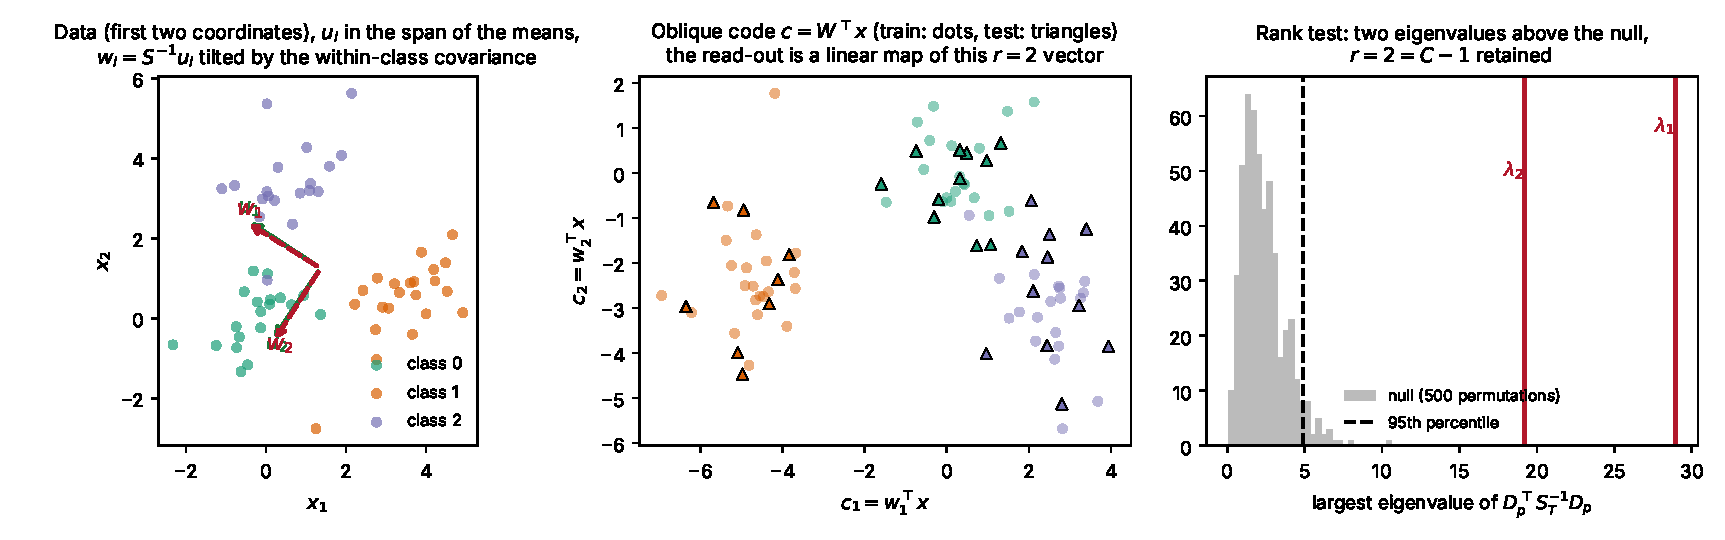
\includegraphics[width=\textwidth]{fig_worked_example.pdf}
\caption{The worked example. Left: training data in the plane of the means
with the representation directions $u_i$ (green) and the measurement
directions $w_i$ (red, dashed); their in-plane tilt is small, the obliquity
is mostly in the third coordinate (not shown), where the noise is correlated
with $x_1$. Centre: the two-dimensional oblique code $c=W^\T x$ on which the
read-out acts; test points are triangles. Right: the rank test, the null
distribution of the largest eigenvalue over 500 label permutations (grey),
its level-$5\%$ threshold (dashed) and the two observed eigenvalues (red),
both far above the null.}
\label{fig:worked}
\end{figure}

%% =====================================================================
\section{Rank selection: structural, tested and used ranks}
\label{sec:rank}
%% =====================================================================
The rank is the only decision of the analytic block
(Figure~\ref{fig:pipeline}). Three different objects are often merged under
the name ``automatic rank'', and they are kept apart here.
\begin{itemize}
  \item The \textbf{structural rank} $r_{\mathrm{struct}}=\min(C-1,d)$ is a
  bound, exact since $\rank S_B\le C-1$. It involves no statistics.
  \item The \textbf{tested rank} $r_{\mathrm{test}}\in\{0,\dots,r_{\mathrm{struct}}\}$
  is the output of a statistical rule. It is a \emph{detection} statement
  (how many discriminant directions are distinguishable from noise at a
  given level) and it may be zero.
  \item The \textbf{used rank} $r_{\mathrm{used}}$ is the number of
  directions the classifier employs. The implementation returns the three
  values; when a tested rule is requested the classifier uses
  $\max(1,r_{\mathrm{test}})$, and the recommended default for prediction
  is $r_{\mathrm{used}}=r_{\mathrm{struct}}$, for the reasons measured in
  Section~\ref{sec:rank-risk}.
\end{itemize}
What is \emph{guaranteed} is limited to two statements: the structural
bound, and the level of the permutation test under the \emph{global} null
hypothesis (no class structure at all). Everything else in this section is
\emph{measured}: the behaviour under alternatives of every rank, the
sequential rule, the Bartlett rule, and the consequences for prediction.

\subsection{The rules}
\paragraph{Permutation test of the global null hypothesis.} The labels are
shuffled $n_{\mathrm{perm}}$ times and the leading generalised eigenvalue
$\lambda^{(p)}_1$ is recomputed for each shuffle. With
$p=(1+\#\{p:\lambda^{(p)}_1\ge\lambda_1\})/(n_{\mathrm{perm}}+1)$, rejecting
when $p\le\alpha$ has level at most $\alpha$ under the global null
hypothesis for every $n$, $d$ and noise distribution, provided the
statistic is computed in the same way for the observed and the shuffled
labels (exchangeability~\cite{phipson2010}). The implementation uses this
exact rule; an interpolated empirical quantile of the shuffled values is
not the same rule and is slightly anti-conservative.

\paragraph{The metric of the test matters.} The natural fast implementation
shares one factorisation of $S_W$ across all permutations (only $S_B$
changes when labels are shuffled). This breaks the proviso above: $S_W$
computed with the true labels excludes exactly the true between-class
direction but not the permuted ones, so the observed statistic is not
exchangeable with the shuffled ones. The remedy costs one factorisation:
use the label-free \emph{total} scatter $S_T$ (shrunk) as the metric of the
test. Without shrinkage, $S_T=S_W+\tfrac{C-1}{n}S_B$ implies that the two
GEVPs share their eigenvectors, with
$\lambda_T=\lambda_W/(1+\tfrac{C-1}{n}\lambda_W)$, an increasing function
of $\lambda_W$: the ordering of the directions and the number of non-zero
eigenvalues are unchanged (with two separate Ledoit--Wolf shrinkages the
identity holds only approximately).

\paragraph{Two extensions beyond rank zero, neither with a guarantee.}
\emph{Max rule} (\texttt{rank="perm"}): every $\lambda_i$ is compared with
the level-$\alpha$ threshold of the \emph{largest} shuffled eigenvalue; the
tested rank is the number of eigenvalues above it. Comparing
$\lambda_2,\lambda_3,\dots$ with the null distribution of a maximum is
expected to be conservative. \emph{Sequential rule with deflation}
(\texttt{rank="seq"}): at step $k$, the $(k+1)$-th eigenvalue is compared
with the distribution, over the shuffles, of the largest eigenvalue
computed after the first $k$ estimated directions have been removed from
the metric; the procedure stops at the first non-rejection. With $(U_k,W_k)$
the biorthogonal pair of the first $k$ directions in the metric of the
test and $P_k=U_kW_k^\T$,
\[
(I-P_k)^\T S^{-1}(I-P_k)=S^{-1}-W_kW_k^\T ,
\]
so that the deflated statistic of a shuffle is the largest eigenvalue of
$M_p-B_p^\T B_p$ with $B_p=W_k^\T D_p$: no new factorisation or solve is
needed. The first step is the exact test above. For $k\ge1$ the labels are
no longer exchangeable under the hypothesis ``rank exactly $k$'' and the
deflation uses estimated directions: the rule is a heuristic, in the
spirit of parallel analysis, whose error rates are measured below.

\paragraph{Bartlett's sequential test} on Wilks' $\Lambda$
(Section~\ref{sec:fast})~\cite{bartlett1947} is analytic and asymptotic.
Information-theoretic criteria such as MDL~\cite{waxkailath1985} play the
same role in array processing; MDL is not reused here because it assumes
isotropic additive noise on the eigenvalues of a covariance, an assumption
foreign to the Fisher GEVP.

\subsection{Calibration under the global null hypothesis}
\begin{table}[h]
\centering\small\renewcommand{\arraystretch}{1.1}
\caption{Probability of a non-zero tested rank on pure noise (nominal level $5\%$; $2000$ independent draws, so that the binomial standard error is $0.5$ point at $5\%$; $199$ or $200$ permutations). Upper part: isotropic Gaussian noise. Lower part: anisotropic Gaussian noise ($\kappa=10$), the null case of Table~\ref{tab:rank-equal}.}
\label{tab:rank-null}
\begin{tabular}{@{}rrrrrrr@{}}
\toprule
$n$ & $d$ & $C$ & permutation, $S_T$ & sequential, $S_T$ & permutation, shared $S_W$ & Bartlett \\
\midrule
30 & 36 & 3 & $3.9\%$ & (same test) & $31.6\%$ & $0.0\%$ \\
60 & 36 & 3 & $4.4\%$ & & $9.7\%$ & $0.0\%$ \\
120 & 36 & 3 & $5.5\%$ & & $6.8\%$ & $0.0\%$ \\
40 & 20 & 4 & $4.5\%$ & & $13.1\%$ & $0.0\%$ \\
120 & 20 & 4 & $4.5\%$ & & $5.2\%$ & $0.2\%$ \\
400 & 20 & 4 & $4.8\%$ & & $5.0\%$ & $2.8\%$ \\
\midrule
40 & 20 & 4 & $4.7\%$ & $4.7\%$ & --- & --- \\
120 & 20 & 4 & $4.8\%$ & $4.8\%$ & --- & --- \\
400 & 20 & 4 & $4.4\%$ & $4.4\%$ & --- & --- \\
\bottomrule
\end{tabular}
\end{table}
The total-scatter permutation test is at its nominal level in the nine
configurations (between $3.9\%$ and $5.5\%$, for a standard error of $0.5$
point), as the theory requires. The shared-$S_W$
variant is anti-conservative as soon as $n$ is not large compared with $d$
(up to $31.6\%$ at $n=30$, $d=36$) and reaches its level only for
$n\gg d$. The Bartlett rule is conservative to the point of never
rejecting when $n$ is of the order of $d$. Under the global null hypothesis
the sequential rule coincides with the max rule (same first step).

\subsection{Rank recovery under alternatives}
\label{sec:rank-recovery}
The global null hypothesis is the least interesting case in practice. The
three rules are therefore evaluated on Gaussian data whose class means
span \emph{exactly} $q$ dimensions, for $q=0,1,2,3$ ($C=4$, $d=20$,
$\kappa=10$, shared covariance), with either equal strengths per direction
(between-class standard deviation $1.2$ along each of the $q$ directions,
in units of the average noise standard deviation) or graded strengths
($1.6$, $0.8$, $0.4$), at $10$, $30$ and $100$ samples per class; $200$
independent draws per cell, $200$ permutations, level $5\%$.
Tables~\ref{tab:rank-equal} and~\ref{tab:rank-graded} report, for each
rule, the probabilities of under-estimating, recovering and
over-estimating $q$.
\begin{table}[h]
\centering\small\renewcommand{\arraystretch}{1.08}
\caption{Rank recovery and predictive risk, \emph{equal} strengths $(1.2,1.2,1.2)$. For each rule: $P(r_{\mathrm{test}}<q)$ / $P(r_{\mathrm{test}}=q)$ / $P(r_{\mathrm{test}}>q)$ in \% over 200 draws (binomial standard error at most $3.5$ points). Right: test accuracy (\%, 2000 test points, centroid read-out) with the rank used by the sequential rule and with $C-1$, and paired differences in points with $95\%$ intervals (conventions of Section~\ref{sec:central}); ``oracle'' is the true rank $q$.}
\label{tab:rank-equal}
\resizebox{\textwidth}{!}{\begin{tabular}{@{}rr|ccc|rrrr@{}}
\toprule
$n$/class & $q$ & max rule & sequential rule & Bartlett & acc., seq. & acc., $C-1$ & seq.\ $-$ $(C-1)$ & $(C-1)$ $-$ oracle \\
\midrule
10 & 0 & $0.0$ / $94.0$ / $6.0$ & $0.0$ / $94.0$ / $6.0$ & $0.0$ / $100.0$ / $0.0$ & -- & -- & -- & -- \\
 & 1 & $0.5$ / $98.5$ / $1.0$ & $0.5$ / $98.5$ / $1.0$ & $99.0$ / $1.0$ / $0.0$ & $44.0$ & $43.9$ & $+0.1\,[-0.1,+0.3]^{\approx}$ & $-0.1\,[-0.3,+0.1]^{\approx}$ \\
 & 2 & $9.5$ / $90.5$ / $0.0$ & $5.0$ / $94.0$ / $1.0$ & $97.0$ / $3.0$ / $0.0$ & $63.3$ & $64.0$ & $-0.8\,[-1.3,-0.2]^{\downarrow}$ & $-0.0\,[-0.2,+0.1]^{\approx}$ \\
 & 3 & $25.5$ / $74.5$ / $0.0$ & $8.5$ / $91.5$ / $0.0$ & $51.5$ / $48.5$ / $0.0$ & $84.8$ & $85.9$ & $-1.1\,[-1.7,-0.6]^{\downarrow}$ & $+0.0\,[+0.0,+0.0]^{\approx}$ \\
\addlinespace
30 & 0 & $0.0$ / $92.0$ / $8.0$ & $0.0$ / $92.0$ / $8.0$ & $0.0$ / $99.0$ / $1.0$ & -- & -- & -- & -- \\
 & 1 & $0.0$ / $100.0$ / $0.0$ & $0.0$ / $98.5$ / $1.5$ & $0.0$ / $98.5$ / $1.5$ & $46.8$ & $46.6$ & $+0.2\,[+0.1,+0.4]^{\approx}$ & $-0.2\,[-0.4,-0.0]^{\approx}$ \\
 & 2 & $0.0$ / $100.0$ / $0.0$ & $0.0$ / $100.0$ / $0.0$ & $0.0$ / $98.5$ / $1.5$ & $68.7$ & $68.7$ & $+0.0\,[-0.1,+0.2]^{\approx}$ & $-0.0\,[-0.2,+0.1]^{\approx}$ \\
 & 3 & $0.0$ / $100.0$ / $0.0$ & $0.0$ / $100.0$ / $0.0$ & $0.0$ / $100.0$ / $0.0$ & $92.3$ & $92.3$ & $+0.0\,[+0.0,+0.0]^{\approx}$ & $+0.0\,[+0.0,+0.0]^{\approx}$ \\
\addlinespace
100 & 0 & $0.0$ / $93.5$ / $6.5$ & $0.0$ / $93.5$ / $6.5$ & $0.0$ / $97.0$ / $3.0$ & -- & -- & -- & -- \\
 & 1 & $0.0$ / $99.5$ / $0.5$ & $0.0$ / $99.0$ / $1.0$ & $0.0$ / $98.5$ / $1.5$ & $47.5$ & $47.4$ & $+0.0\,[-0.1,+0.2]^{\approx}$ & $-0.1\,[-0.2,+0.1]^{\approx}$ \\
 & 2 & $0.0$ / $100.0$ / $0.0$ & $0.0$ / $99.5$ / $0.5$ & $0.0$ / $97.0$ / $3.0$ & $70.3$ & $70.2$ & $+0.1\,[-0.0,+0.2]^{\approx}$ & $-0.1\,[-0.2,+0.0]^{\approx}$ \\
 & 3 & $0.0$ / $100.0$ / $0.0$ & $0.0$ / $100.0$ / $0.0$ & $0.0$ / $100.0$ / $0.0$ & $94.4$ & $94.4$ & $+0.0\,[+0.0,+0.0]^{\approx}$ & $+0.0\,[+0.0,+0.0]^{\approx}$ \\
\bottomrule
\end{tabular}}
\end{table}
\begin{table}[h]
\centering\small\renewcommand{\arraystretch}{1.08}
\caption{Rank recovery and predictive risk, \emph{graded} strengths $(1.6,0.8,0.4)$. Same conventions as Table~\ref{tab:rank-equal}.}
\label{tab:rank-graded}
\resizebox{\textwidth}{!}{\begin{tabular}{@{}rr|ccc|rrrr@{}}
\toprule
$n$/class & $q$ & max rule & sequential rule & Bartlett & acc., seq. & acc., $C-1$ & seq.\ $-$ $(C-1)$ & $(C-1)$ $-$ oracle \\
\midrule
10 & 0 & $0.0$ / $94.0$ / $6.0$ & $0.0$ / $94.0$ / $6.0$ & $0.0$ / $100.0$ / $0.0$ & -- & -- & -- & -- \\
 & 1 & $0.0$ / $99.0$ / $1.0$ & $0.0$ / $99.0$ / $1.0$ & $89.0$ / $11.0$ / $0.0$ & $47.7$ & $47.6$ & $+0.1\,[-0.1,+0.2]^{\approx}$ & $-0.1\,[-0.2,+0.1]^{\approx}$ \\
 & 2 & $53.5$ / $46.5$ / $0.0$ & $37.0$ / $63.0$ / $0.0$ & $100.0$ / $0.0$ / $0.0$ & $56.7$ & $60.9$ & $-4.2\,[-5.0,-3.4]^{\downarrow}$ & $+0.2\,[-0.0,+0.5]^{\approx}$ \\
 & 3 & $100.0$ / $0.0$ / $0.0$ & $98.0$ / $2.0$ / $0.0$ & $100.0$ / $0.0$ / $0.0$ & $57.5$ & $66.3$ & $-8.9\,[-9.7,-8.0]^{\downarrow}$ & $+0.0\,[+0.0,+0.0]^{\approx}$ \\
\addlinespace
30 & 0 & $0.0$ / $92.0$ / $8.0$ & $0.0$ / $92.0$ / $8.0$ & $0.0$ / $99.0$ / $1.0$ & -- & -- & -- & -- \\
 & 1 & $0.0$ / $99.5$ / $0.5$ & $0.0$ / $99.0$ / $1.0$ & $0.0$ / $98.5$ / $1.5$ & $49.0$ & $49.0$ & $+0.1\,[-0.1,+0.2]^{\approx}$ & $-0.1\,[-0.2,+0.1]^{\approx}$ \\
 & 2 & $0.0$ / $100.0$ / $0.0$ & $0.0$ / $100.0$ / $0.0$ & $0.0$ / $98.5$ / $1.5$ & $66.0$ & $65.9$ & $+0.1\,[-0.1,+0.2]^{\approx}$ & $-0.1\,[-0.2,+0.1]^{\approx}$ \\
 & 3 & $69.0$ / $31.0$ / $0.0$ & $50.0$ / $50.0$ / $0.0$ & $34.0$ / $66.0$ / $0.0$ & $71.2$ & $74.4$ & $-3.3\,[-3.8,-2.8]^{\downarrow}$ & $+0.0\,[+0.0,+0.0]^{\approx}$ \\
\addlinespace
100 & 0 & $0.0$ / $93.5$ / $6.5$ & $0.0$ / $93.5$ / $6.5$ & $0.0$ / $97.0$ / $3.0$ & -- & -- & -- & -- \\
 & 1 & $0.0$ / $99.5$ / $0.5$ & $0.0$ / $99.0$ / $1.0$ & $0.0$ / $98.5$ / $1.5$ & $49.3$ & $49.3$ & $-0.0\,[-0.2,+0.2]^{\approx}$ & $+0.0\,[-0.2,+0.2]^{\approx}$ \\
 & 2 & $0.0$ / $100.0$ / $0.0$ & $0.0$ / $99.5$ / $0.5$ & $0.0$ / $97.0$ / $3.0$ & $67.9$ & $67.8$ & $+0.1\,[+0.0,+0.3]^{\approx}$ & $-0.1\,[-0.3,-0.0]^{\approx}$ \\
 & 3 & $0.0$ / $100.0$ / $0.0$ & $0.0$ / $100.0$ / $0.0$ & $0.0$ / $100.0$ / $0.0$ & $78.5$ & $78.5$ & $+0.0\,[+0.0,+0.0]^{\approx}$ & $+0.0\,[+0.0,+0.0]^{\approx}$ \\
\bottomrule
\end{tabular}}
\end{table}
\begin{itemize}
  \item \textbf{Over-estimation is rare for $q\ge1$.} It never exceeds
  $1.5\%$ for the two permutation rules and $3\%$ for Bartlett. (In the
  rows $q=0$ the over-estimation rate is the false-positive rate of the
  global null hypothesis; the values $6$ to $8\%$ rest on $200$ draws and
  are compatible with the $4.4$ to $4.8\%$ measured on $2000$ draws of the
  same configurations in Table~\ref{tab:rank-null}.)
  \item \textbf{Under-estimation is the failure mode, and it can be
  total.} With equal strengths and $10$ samples per class the max rule
  misses a direction in $25.5\%$ of the draws at $q=3$, the sequential
  rule in $8.5\%$, Bartlett in $51.5\%$ (and in $97$ to $99\%$ at $q=1$
  and $2$, where it almost never rejects). With graded strengths the weak
  directions are simply not detected at small $n$: at $10$ per class and
  $q=3$ no rule recovers the rank in more than $2\%$ of the draws (mean
  tested rank $1.50$, $1.66$ and $0.82$), and at $30$ per class the third
  direction is found in $31\%$, $50\%$ and $66\%$ of the draws. At $100$
  per class the three rules recover every rank $q\ge1$ in at least $97\%$
  of the draws.
  \item \textbf{The sequential rule dominates the max rule}: it never
  under-estimates more often, and less often wherever the two differ (for
  instance $8.5\%$ against $25.5\%$, $37\%$ against $53.5\%$, $50\%$
  against $69\%$), at the price
  of an over-estimation rate of at most $1.5\%$. Bartlett has no power
  when $n$ is of the order of $d$ and becomes the most powerful of the
  three at $30$ per class on the weakest direction, with an
  over-estimation rate of $1.5$ to $3\%$ at larger $n$.
\end{itemize}
A tested rank is therefore a statement of the form ``at least
$r_{\mathrm{test}}$ directions are detectable at this sample size'', with
a small probability of over-statement; it is not an estimate of the true
rank when directions are weak relative to $n$.

\subsection{Rank error is not predictive risk}
\label{sec:rank-risk}
The right-hand columns of Tables~\ref{tab:rank-equal}
and~\ref{tab:rank-graded} answer a different question: which rank should
the classifier \emph{use}? Three facts stand out.
\begin{itemize}
  \item \textbf{Keeping all $C-1$ directions costs almost nothing when the
  true rank is lower.} The difference between the structural rank and the
  oracle rank $q$ lies between $-0.2$ and $+0.2$ point in the eighteen
  cells, always inside the equivalence margin: the centroid read-out is
  barely affected by one or two pure-noise coordinates.
  \item \textbf{Using a tested rank gains at most $0.2$ point} when the
  test is right and the true rank is below $C-1$.
  \item \textbf{Using a tested rank costs up to $8.9$ points} when the
  test lacks power: $-0.8$ and $-1.1$ point with equal strengths at $10$
  per class, and $-4.2$, $-8.9$ and $-3.3$ points with graded strengths
  (at $10$ per class for $q=2,3$, and at $30$ per class for $q=3$), all
  with intervals excluding zero. A weak direction that is not
  \emph{detectable} at level $5\%$ still carries information that the
  classifier can use.
\end{itemize}
The asymmetry is the practical conclusion of this section: for prediction
the used rank should be the structural rank $C-1$, and the tested rank
should be reported as what it is, a detection result. The same asymmetry
is observed on the digits data (Section~\ref{sec:central}) and in the
small-sample diagnosis of Section~\ref{sec:small}, where an
under-estimated rank is one of the three causes of the accuracy loss.

\subsection{Families of tests: per-block and family-wise control}
\label{sec:rank-fwer}
When one block is fitted per frequency band, per sensor group or per
subject, and each block is retained if its own test rejects, the tests
form a family. A test at level $5\%$ \emph{per block} controls the rate of
false selections per null block, not the probability of selecting at least
one null block, which grows with the size of the family. A family-wise
control is obtained without additional computation by the single-step
min-$p$ procedure~\cite{westfall1993}: the same label permutations are
used for all blocks, every statistic (observed or shuffled) is converted
into a $p$-value within its own block, and the adjusted $p$-value of a
block is the proportion of labellings (observed one included) whose
smallest $p$-value over the family is at most the $p$-value of that
block. Under the global null hypothesis the probability of retaining at
least one block is then at most $\alpha$, again by exchangeability.

Measured on families of eight independent blocks ($d=36$, $C=3$, $n=30$,
$200$ draws, $200$ permutations):
\begin{center}\small
\begin{tabular}{@{}lrr@{}}
\toprule
 & per-block test & min-$p$ control \\
\midrule
all blocks null: $P(\text{at least one block retained})$ & $33.0\%$ & $3.5\%$ \\
all blocks null: selection rate per block & $5.1\%$ & $0.5\%$ \\
one informative block: $P(\text{at least one null block retained})$ & $27.5\%$ & $2.5\%$ \\
one informative block: power on that block & $100\%$ & $100\%$ \\
\bottomrule
\end{tabular}
\end{center}
The per-block test behaves as designed ($5.1\%$ per block, hence
$33.0\%$ for the family, for an expected $1-0.95^8=33.7\%$ under
independence); the min-$p$ control brings the family-wise rate to $3.5\%$
with no loss of power in this configuration, where the informative block
is strong. Which control is appropriate depends on the use: a per-block
level is acceptable when false selections merely add noise coordinates to
a downstream classifier, a family-wise level is required when the
selection itself is the finding (``this band is discriminant''). Both are
available in the implementation (\texttt{fwer\_select}), and
Appendix~\ref{sec:fourier} reports both for the frequency-band experiment.

\paragraph{Summary of the guarantees.}
\begin{center}\small\renewcommand{\arraystretch}{1.15}
\begin{tabular}{@{}p{0.36\linewidth}p{0.27\linewidth}p{0.31\linewidth}@{}}
\toprule
\textbf{Statement} & \textbf{Status} & \textbf{Where it fails} \\
\midrule
$r\le C-1$ & exact & --- \\
$P(r_{\mathrm{test}}>0)\le\alpha$ under the global null hypothesis ($S_T$ metric, exact $p$-value) & proved (exchangeability), checked on $2000$ draws & shared-$S_W$ metric; interpolated quantile \\
family-wise level of the min-$p$ selection under the global null hypothesis & proved, checked on $200$ draws & --- \\
$P(r_{\mathrm{test}}>q)$ small for a true rank $q\ge1$ & measured ($\le1.5\%$ for the permutation rules in the cases tested) & no proof; other distributions not tested \\
$r_{\mathrm{test}}=q$ & measured & weak directions at small $n$ (down to $0$--$2\%$ recovery) \\
tested rank optimal for prediction & \emph{not supported} & costs up to $8.9$ points when the test lacks power \\
\bottomrule
\end{tabular}
\end{center}

%% =====================================================================
\section{Limits of oblique projectors and their control in the analytic block}
\label{sec:stability}
%% =====================================================================
Oblique projectors have intrinsic limits that no construction removes: they
can amplify noise, they discard the kernel irreversibly, they are not
Euclidean best approximations, and they are a very constrained class of
linear maps. This section states these limits precisely, separates what is
intrinsic from what depends on how the blocks are assembled, and shows how
the analytic construction bounds or mitigates them. Every statement is
verified numerically (\texttt{ropn\_auto\_stabilite.py}); the measurements
are reported with the statements.

\subsection{Noise amplification: norm and angle}
\begin{proposition}[Norm of an oblique projector]
\label{prop:norm-angle}
Let $P=U(W^\T U)^{-1}W^\T$ with $U,W\in\R^{d\times r}$ of full rank, $W^\T U$
invertible, $0<r<d$, and let $Q_U,Q_W$ be orthonormal bases of $\spn U$ and
$\spn W$. Then
\begin{equation}
  \|P\|_2=\frac1{\sigma_{\min}(Q_W^\T Q_U)}=\frac1{\sin\theta_{\min}},\qquad
  \|I-P\|_2=\|P\|_2,
  \label{eq:norm-angle}
\end{equation}
where $\theta_{\min}$ is the smallest principal angle between $\im P=\spn U$
and $\ker P=(\spn W)^\perp$. More precisely, the non-zero singular values of
$P$ are $1/\cos\theta_i$, $i=1,\dots,r$, where the $\theta_i$ are the
principal angles between $\spn U$ and $\spn W$. The amplification bound
$\|P(x+\delta x)-Px\|_2\le\|P\|_2\|\delta x\|_2$ is attained along the
dominant right singular vector of $P$.
\end{proposition}
\begin{proof}
$P$ depends only on the two subspaces, so $P=Q_U(Q_W^\T Q_U)^{-1}Q_W^\T$;
since $Q_U$ has orthonormal columns and $Q_W^\T$ orthonormal rows, the
singular values of $P$ are those of $(Q_W^\T Q_U)^{-1}$, i.e.\ the inverses
of the singular values of $Q_W^\T Q_U$, which are the cosines of the
principal angles between $\spn U$ and $\spn W$; hence
$\|P\|_2=1/\sigma_{\min}(Q_W^\T Q_U)$. With $Q_\perp$ an orthonormal basis of
$(\spn W)^\perp=\ker P$,
$Q_U^\T Q_\perp Q_\perp^\T Q_U=I-Q_U^\T Q_WQ_W^\T Q_U$, so the largest
singular value of $Q_\perp^\T Q_U$, which is the cosine of the smallest
principal angle $\theta_{\min}$ between $\spn U$ and $\ker P$, satisfies
$\cos^2\theta_{\min}=1-\sigma_{\min}^2(Q_W^\T Q_U)$, i.e.\
$\sigma_{\min}(Q_W^\T Q_U)=\sin\theta_{\min}$. The identity
$\|I-P\|_2=\|P\|_2$ for $P\ne0,I$ is classical~\cite{szyld2006,ipsenmeyer1995}.
The bound is attained because $\|P\|_2$ is by definition the maximum of
$\|P\delta x\|/\|\delta x\|$.
\end{proof}
Two consequences deserve emphasis. First, eigenvalues confined to $\{0,1\}$
say nothing about amplification: $P_a=\begin{pmatrix}1&a\\0&0\end{pmatrix}$
is idempotent with eigenvalues $0$ and $1$, yet $\|P_a\|_2=\sqrt{1+a^2}$ and
the perturbation $(0,\varepsilon)$ becomes $(a\varepsilon,0)$ (verified for
$a=0,1,10$: norms $1$, $1.4142$, $10.0499$). Second, the condition number of
the cross-Gram $W^\T U$ is not an obliquity measure either: at rank one it is
always $1$, and in the biorthogonal gauge of this report it is $1$ at every
rank by construction, while $\|P\|_2$ can be arbitrary (with $u=e_1$ and
$w=u+t\,e_2$, $w^\T u=1$ and $\|P\|_2=\sqrt{1+t^2}$: $1.41$, $5.10$, $50.01$
for $t=1,5,50$). This is why the report measures
$\sigma_{\min}(Q_W^\T Q_U)$ and $\|P\|_2$, never $\kappa(W^\T U)$. On the
analytic block ($d=20$, $C=4$, $n=100$ per class) the three expressions
of~\eqref{eq:norm-angle} agree to four digits ($1.1614$ at $\kappa=10$,
$1.5469$ at $\kappa=200$), $\|I-P\|_2$ equals $\|P\|_2$, and the measured
amplification along the dominant singular direction equals the bound.

\subsection{The interpolation threshold: where the raw projector's norm peaks}
Rocks and Mehta~\cite{rocksmehta2021} showed that in over-parameterised
least-squares regression with linear random features, in the ridge-less
limit, the fitted map is an oblique projector whose singular values
$1/\cos\theta_i$ diverge at the interpolation threshold (number of
parameters equal to the number of samples), because one subspace
orientation angle approaches $90^\circ$; they relate this divergence to the
double-descent peak of the test error. (That an explicit ridge penalty
attenuates such a peak is a classical observation, not a result of that
paper.) The analytic block has its own interpolation threshold: the
within-class scatter $S_W$ has rank at most $\min(n_{\mathrm{train}}-C,d)$,
with equality almost surely for data with a density, so at
$n_{\mathrm{train}}-C\approx d$ it becomes full rank with a very small
smallest eigenvalue, and the raw Fisher projector (metric $S_W^{+}$) is
strongly oblique. Measured ($d=20$, $C=4$, $\kappa(S_W)=200$, 20 seeds,
Figure~\ref{fig:dd}): the norm of the raw projector rises from $3.3$ at
$(n_{\mathrm{train}}-C)/d=0.75$ to $4.7$ at $1.05$ and falls back to $3.5$ at
$1.2$ and $2.2$ at large $n$; below the threshold it rises again as the
pseudo-inverse acts on an ever smaller subspace ($7.5$ at $0.2$). The shrunk
projector is flat ($1.26$--$1.57$) throughout: Ledoit--Wolf shrinkage plays
for the oblique block a role analogous to that of ridge regularisation in
regression. The test accuracy of the raw block (centroid read-out) falls
from $100\%$ to $45\%$ as $n$ decreases, with a small dip at the threshold
($88.9\%$, $85.5\%$ and $89.1\%$ at $(n_{\mathrm{train}}-C)/d=0.75$, $0.90$
and $1.05$) that is of the order of the standard error of these means
(about $2.5$ points on $20$ seeds of about ten test points each) and is
therefore not established; a read-out on a low-dimensional code may simply
be more tolerant than a regression on the full state. The norm peak
nonetheless signals the regime to avoid. The shrunk block is less oblique
everywhere, much more accurate below the threshold ($84$--$99\%$ against
$45$--$89\%$ for $(n_{\mathrm{train}}-C)/d\le0.9$) and equivalent well above
it (within $0.3$ point for $(n_{\mathrm{train}}-C)/d\ge1.45$).
\begin{figure}[t]
\centering
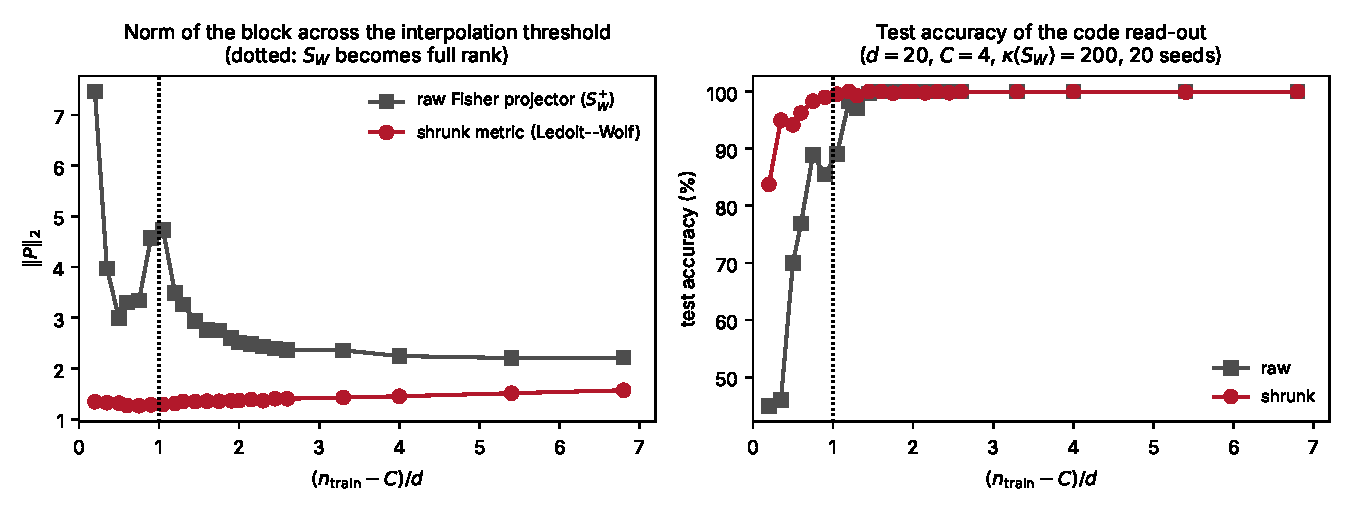
\includegraphics[width=\textwidth]{fig_double_descent.pdf}
\caption{The interpolation threshold of the analytic block. Left: spectral
norm of the raw Fisher projector (pseudo-inverse of $S_W$, grey) and of the
shrunk projector (red) as a function of $(n_{\mathrm{train}}-C)/d$; the raw
norm peaks where $S_W$ becomes full rank with a vanishing smallest
eigenvalue (dotted line), the shrunk norm is flat. Right: test accuracy of the
centroid read-out of the code for the two metrics.}
\label{fig:dd}
\end{figure}

\subsection{What bounds the obliquity: the metric}
The analytic block is never an arbitrary oblique projector: it is the
$M$-orthogonal projector for $M=S^{-1}$, $S$ the (shrunk) within-class
scatter. This bounds its norm.
\begin{proposition}[Metric bound on the norm]
\label{prop:metric-bound}
If $P$ is $M$-orthogonal ($W=MU$, $M\succ0$, $0<r<d$) and
$\kappa=\kappa(M)$, then
\begin{equation}
  \|P\|_2\ \le\ \frac12\Bigl(\sqrt{\kappa}+\frac1{\sqrt{\kappa}}\Bigr)\ \le\ \sqrt{\kappa},
  \label{eq:metric-bound}
\end{equation}
and, for $\kappa>1$, the first inequality is an equality for a suitable
rank-one projector.
For the analytic block with Ledoit--Wolf shrinkage,
$S=(1-a)S_W+a\mu I$ with $a\mu>0$, $\kappa=\kappa(S)$ and
\begin{equation}
  \sqrt{\kappa(S)}\le\sqrt{1+\frac{(1-a)\lambda_{\max}(S_W)}{a\mu}}.
  \label{eq:shrink-bound}
\end{equation}
\end{proposition}
\begin{proof}
$\ker P=(\spn W)^\perp=\{y:\ y^\T Mu=0\ \forall u\in\spn U\}$ is the
$M$-orthogonal complement of $\im P$. Wielandt's
inequality~\cite[Section~7.4]{hornjohnson2013}, applied to $M^{-1}$ and to the
Euclidean-orthogonal vectors $M^{1/2}x$, $M^{1/2}y$, states that
$|x^\T y|\le\frac{\kappa-1}{\kappa+1}\|x\|\|y\|$ whenever $x^\T My=0$. The
smallest principal angle between $\im P$ and $\ker P$ therefore satisfies
$\cos\theta_{\min}\le\frac{\kappa-1}{\kappa+1}$, i.e.\
$\sin\theta_{\min}\ge\frac{2\sqrt\kappa}{\kappa+1}$, and
Proposition~\ref{prop:norm-angle} gives
$\|P\|_2=1/\sin\theta_{\min}\le\frac{\kappa+1}{2\sqrt\kappa}$, which is at
most $\sqrt\kappa$ since $\kappa\ge1$. Equality holds at rank one for
$u=v_{\min}/\sqrt{\lambda_{\min}}+v_{\max}/\sqrt{\lambda_{\max}}$, with
$(\lambda_{\min},v_{\min})$ and $(\lambda_{\max},v_{\max})$ the extreme
eigenpairs of $M$ (the equality case of the Kantorovich inequality). (The
weaker bound $\sqrt\kappa$ also follows directly from the fact that
$M^{1/2}PM^{-1/2}$ is an orthogonal projector.) Finally, with $M=S^{-1}$,
$\kappa(M)=\kappa(S)$, $\lambda_{\min}(S)\ge a\mu$ and
$\lambda_{\max}(S)\le(1-a)\lambda_{\max}(S_W)+a\mu$.
\end{proof}
The shrinkage coefficient therefore sets the \emph{admissible obliquity}:
the data-driven choices of the block concern not only the rank but,
through $a$, its norm. Measured ($\kappa(S_W)=200$ at the population level,
10 seeds):
\begin{center}
\small
\begin{tabular}{rrrrrrrr}
\toprule
$n$/class & $a$ (LW) & $\|P\|_2$ raw $S_W$ & $\|P\|_2$ shrunk & bound~\eqref{eq:metric-bound} & $\sqrt{\kappa(S)}$ & bound~\eqref{eq:shrink-bound} & $\sqrt{\kappa(S_W)}$ \\
\midrule
10 & 0.278 & 3.09 & 1.32 & 2.27 & 4.31 & 4.32 & 68.7 \\
15 & 0.217 & 2.53 & 1.30 & 2.50 & 4.78 & 4.85 & 28.1 \\
30 & 0.132 & 2.16 & 1.41 & 3.00 & 5.84 & 6.14 & 18.5 \\
100 & 0.045 & 2.02 & 1.62 & 4.31 & 8.51 & 10.33 & 15.0 \\
1000 & 0.005 & 1.96 & 1.90 & 6.54 & 13.01 & 32.71 & 14.2 \\
\bottomrule
\end{tabular}
\end{center}
\begin{figure}[t]
\centering
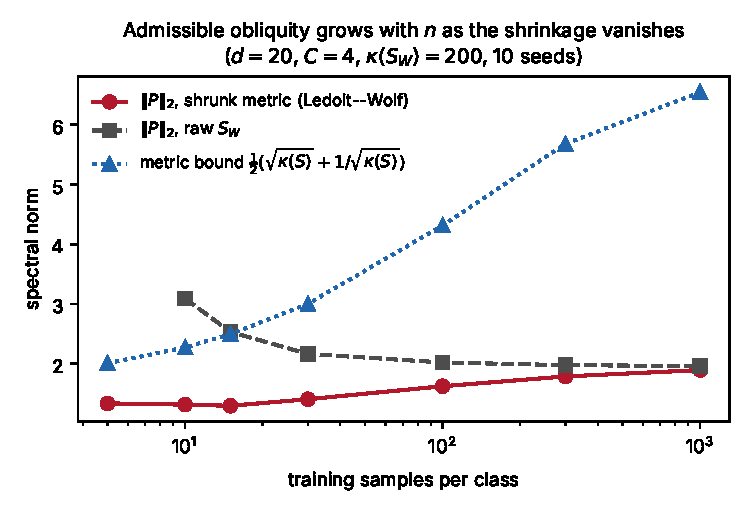
\includegraphics[width=0.6\textwidth]{fig_norm_vs_n.pdf}
\caption{Admissible obliquity as a function of the sample size: spectral
norm of the shrunk Fisher projector (red), of the raw Fisher projector
(grey, computed only where $S_W$ is invertible, $n_{\mathrm{train}}>d+C$) and
the metric bound $\tfrac12(\sqrt{\kappa(S)}+1/\sqrt{\kappa(S)})$ of
Proposition~\ref{prop:metric-bound} (blue).}
\label{fig:norm}
\end{figure}
The bound~\eqref{eq:metric-bound} holds for every seed
(Figure~\ref{fig:norm}; it is attained to four digits by the rank-one
example of the proof, and never exceeded on $2000$ random pairs $(M,U)$),
and $M$-orthogonality is exact
($\|MP-P^\T M\|/\|MP\|\le2.3\times10^{-15}$). As $n$ grows the coefficient $a$
decreases, the admissible obliquity grows, and the measured norm rises from
$1.3$ to $1.9$, towards the value of the raw projector; at small $n$ the raw
projector ($\|P\|_2=3.1$ at $10$ per class) is replaced by a much less
oblique one ($1.3$). The bound is far from the measured norm at large $n$
(the extreme eigen-directions of the metric are not aligned with the
discriminant directions); what it establishes is the mechanism: shrinkage
is a control of the norm, by the same coefficient that improves the
accuracy at $\kappa=10$ in Section~\ref{sec:small}.

\subsection{Best approximation: not Euclidean, but in the Fisher metric}
The orthogonal projector $Q_S$ onto the subspace $\im P$ (here $Q_S$ denotes
a projector, not a basis) returns the Euclidean nearest point of $\im P$; an
oblique projector onto the same subspace does not. Since
$(I-P)Q_Sx=0$, one has $x-Px=(I-P)(x-Q_Sx)$ and therefore
\begin{equation}
  \|x-Px\|_2\le\|I-P\|_2\,\|x-Q_Sx\|_2=\|P\|_2\,\|x-Q_Sx\|_2 .
  \label{eq:best-approx}
\end{equation}
The reconstruction penalty is governed by the same norm that governs noise
amplification. Measured on the block ($\kappa=200$, $n=100$ per class): the
ratio $\|x-Px\|/\|x-Q_Sx\|$ lies in $[1.005,1.354]$ on the test set, below
$\|P\|_2=1.547$, and exceeds one at every point. In the Fisher norm
$\|v\|_M=\sqrt{v^\T Mv}$, however, the same ratio lies in $[0.526,0.986]$:
the $M$-orthogonal projector \emph{is} the best approximation in its own
metric. Obliquity is therefore justified by the task metric, not by any
general approximation property; the block minimises the reconstruction
error in the (shrunk) within-class Mahalanobis norm, the natural norm for a
discriminant representation under the shared-covariance model, and pays for
it in Euclidean error by at most the factor $\|P\|_2$.

\subsection{Information loss and the residual form}
For $r<d$, two inputs that differ by a kernel component are
indistinguishable after projection, and no later block can recover what a
projector has removed unless another path carries it. In the vocabulary of
Rocks and Mehta~\cite{rocksmehta2021}, every input perturbation splits into
an \emph{invariant} component in $\ker P$, which leaves the prediction
unchanged, and an \emph{adversarial} component in $(\ker P)^\perp=\spn(W)$,
which changes it; the invariant subspace is a consequence of the model's
bias, i.e.\ of what the block has decided not to read. In the analytic
block the read-out acts on the code, so the kernel is discarded
\emph{deliberately}: a perturbation of norm $3\sigma$ confined to
$\ker W^\T$ changes the code by $3\times10^{-14}$ and leaves $100\%$ of the
predictions unchanged, while a perturbation of the same norm inside $\spn U$
changes $26\%$ of them (centroid read-out). The most effective perturbation of a given norm is
along the dominant left singular direction of $W$, and its effect on the code
is bounded by $\sigma_{\max}(W)\|\delta x\|$. This is Proposition~\ref{prop:code}(i) read as a
risk: a direction that is useless on the training distribution but
informative out of distribution is lost. The justification is statistical,
not architectural: on data for which LDA is Bayes-optimal the Fisher code is
a sufficient statistic (Section~\ref{sec:reinjection}); on other data the
lattice (Appendix~\ref{sec:lattice}) or per-class metrics
(Appendix~\ref{sec:alternatives}) must re-expose the kernel through a fixed
non-linearity. The residual form $I+P/L$ keeps the kernel but is no
longer a projector: with $\mathcal T=I+P/L$,
$\|\mathcal T^2-\mathcal T\|/\|\mathcal T\|=0.86$, $0.37$, $0.16$ for
$L=1,2,4$. It is, however, invertible in closed form,
\begin{equation}
  (I+P/L)^{-1}=I-\frac{P}{L+1},\qquad\det(I+P/L)=(1+1/L)^r,
  \label{eq:resid-inverse}
\end{equation}
(verified to $1.5\times10^{-15}$ and to all displayed digits of the
determinant), which is why the linear recursion of
Section~\ref{sec:recursion} does not lose rank, although it remains a
single affine function of $P$ (Theorem~\ref{thm:collapse}).

\subsection{Regularising the cross-Gram versus regularising the metric}
A tempting numerical safeguard is to replace $(W^\T U)^{-1}$ by
$(W^\T U+\lambda I)^{-1}$. This destroys idempotence: on the analytic
block, $\|P^2-P\|/\|P\|=9.9\times10^{-3}$, $9.1\times10^{-2}$ and
$0.50$ for $\lambda=10^{-2}$, $10^{-1}$ and $1$, against $1.9\times10^{-16}$
for $\lambda=0$ (in the biorthogonal gauge this ratio is exactly
$\lambda/(1+\lambda)$). Such an operator is a regularised projection-like
map, and the results of Section~\ref{sec:recursion}, whose proofs use
$P^2=P$, do not apply to it as they stand. The analytic block never does this: its
regularisation enters the \emph{metric} ($S_W\to(1-a)S_W+a\mu I$), the
cross-Gram is fixed at $I_r$ by construction, and idempotence stays exact
($\|P^2-P\|/\|P\|=10^{-15}$, $\|W^\T U-I\|=1.7\times10^{-15}$ with
$a=0.045$). The price, documented in Section~\ref{sec:audit}, is that the
operator is the shrunk Fisher projector, not the raw one.

\subsection{Expressivity and depth}
A projector is a very constrained linear map: identity on its image, zero on
its kernel, $P^k=P$, the composition of fixed projectors without
non-linearity is linear and of rank at most the smallest factor rank. The
expected benefit is a geometric inductive bias, not an automatic gain in
expressivity over a free linear layer; Theorems~\ref{thm:collapse}
and~\ref{thm:A} make this precise for the shared-weight case, and the
unconstrained low-rank control of Section~\ref{sec:audit} indicates that, on
clean data, the accuracy comes from the metric, not from idempotence. In depth, the product
bound $\|P_L\cdots P_1\|_2\le\prod_\ell\|P_\ell\|_2$ shows why moderate
amplification per layer is not a global guarantee; for the shared block the
exact value is available and the bound is loose
($\|(I+P/L)^L\|_2=2.75$, $3.03$, $3.22$ against $(1+\|P\|_2/L)^L=3.15$,
$3.70$, $4.11$ for $L=2,4,8$). Finally, invertibility, stability and
conditioning are three different properties: the un-normalised gated
recursion $h\leftarrow(1-a)h+aPh$ with the analytic gate ($s\in\spn(W)$,
for which Theorem~\ref{thm:gate-det} gives a positive determinant
$(1-a)^{d-r}$ per step) has a non-zero determinant at every depth, yet its
smallest singular value falls from $0.38$ ($T=1$) to $0.018$ ($T=8$) and its
condition number rises from $4.3$ to $84.9$ on the same input. (For a gate
that reads the residual, the determinant can vanish, as in
Example~\ref{ex:det}.) A non-zero determinant excludes rank collapse; it
says nothing about conditioning. The condition number of the global
Jacobian is the quantity to report, and Section~\ref{sec:audit} does so,
including for the residual-normalised gate, which behaves very
differently.

%% =====================================================================
\section{What each ingredient contributes}
\label{sec:ingredients}
%% =====================================================================
A natural objection to the construction is: why speak of a network of
projectors if the final predictor only uses the classical discriminant
directions? At inference with a read-out on the code, $U$ is indeed not
even needed: one computes $W^\T x$ and applies a linear read-out. The
answer is that three ingredients are present, that they do different
things, and that the experimental gains must be attributed to the right
one.
\begin{center}\small\renewcommand{\arraystretch}{1.2}
\begin{tabular}{@{}p{0.19\linewidth}p{0.36\linewidth}p{0.38\linewidth}@{}}
\toprule
\textbf{Ingredient} & \textbf{What it brings} & \textbf{Evidence in this report} \\
\midrule
\textbf{Fisher metric} $W=S^{-1}U$ (with shrinkage) &
\emph{Prediction accuracy.} It is the whole of the statistical content: the
block is LDA (Proposition~\ref{prop:lda}). &
The orthogonal variant with the same image loses $4$ to $6$ points at
$\kappa=200$, while an unconstrained low-rank map fitted with a ridge does
as well as the block on clean data in three cases out of four
(Section~\ref{sec:audit}, R6). The
block is equivalent to shrinkage LDA in the central benchmark
(Section~\ref{sec:central}). \\
\textbf{Factorisation} ($C\times C$ reduction, dual form) &
\emph{Computation.} Exactly the same estimator at a lower cost; nothing
statistical. &
One to three orders of magnitude against a dense generalised
eigen-decomposition, but a factor $5$ to $11$ against scikit-learn's
shrinkage LDA solver when $n\ge d$, and more only when $n\ll d$
(Section~\ref{sec:fast-lda}); batched permutations make the rank test
affordable. \\
\textbf{Idempotence} $W^\T U=I_r$, $P^2=P$ &
\emph{Exact structural statements}: the theorems of
Section~\ref{sec:recursion}, the norm identities and the metric bound of
Section~\ref{sec:stability}, the invariance of the code. No accuracy by
itself. &
Fine-tuning with or without the idempotence constraint gives the same or a
lower accuracy than the analytic block (Section~\ref{sec:reinjection});
the unconstrained low-rank control matches it on clean data. \\
\bottomrule
\end{tabular}
\end{center}
In short: the accuracy is that of the metric, the speed is that of the
factorisation, and the projector structure is what makes the recurrences of
Section~\ref{sec:recursion} analysable in closed form. The projector
structure is used by the predictor only when the state $h$ itself is
propagated (recursion, residual, lattices of Appendix~\ref{sec:lattice});
for a single block read on its code, the projector is an interpretation of
LDA, not an additional mechanism.

%% =====================================================================
\section{Central benchmark: symmetric comparisons with paired uncertainty}
\label{sec:central}
%% =====================================================================
This section is the empirical core of the report. It tests one promise:
\emph{the analytic block remains useful at small $n$ when its assumptions
(Gaussian classes with a common covariance) hold only approximately}. The
other experiments of the report are diagnoses (Section~\ref{sec:small}) or
demonstrations (appendices).

\subsection{Protocol}
\textbf{Data.} (a)~Synthetic problems with $C=4$, $d=20$, $\kappa=50$ and
$n=15$ or $60$ training samples per class, each realisation being an
\emph{independent draw} of the whole problem (means, covariances, samples)
evaluated on $2000$ fresh test points, so that the test noise is small:
Gaussian classes with a shared covariance (assumptions satisfied);
heteroscedastic classes, one covariance orientation per class (shared
covariance violated); Student $t_3$ noise with a common scatter
(Gaussianity violated); proportional covariances with factors
$0.4,0.8,1.4,2.4$ (mild violation). (b)~One real dataset, the largest
available offline in the execution environment: scikit-learn's
\texttt{digits} ($1797$ images $8\times8$, ten classes, $61$ non-constant
features), with repeated stratified subsamples of $10$, $30$ or $100$
training images per class and all remaining images as test set. These
repetitions measure the variability of the subsample; they are not
independent realisations of the problem, and the intervals below must be
read accordingly.

\textbf{Methods.} The analytic block (Ledoit--Wolf shrinkage of the pooled
within-class scatter, rank $C-1$) with the centroid read-out, i.e.\ LDA; the
same block with the least-squares read-out; scikit-learn's shrinkage LDA
(\texttt{lsqr}, which shrinks each class covariance separately before
averaging, Section~\ref{sec:lda}); multinomial logistic
regression; an MLP with one hidden layer.

\textbf{Two separate comparisons.} \emph{Without tuning}: one default
recipe per method, fixed before the experiments (block: Ledoit--Wolf; LDA:
\texttt{shrinkage="auto"}; logistic regression: $C=1$; MLP: scikit-learn
defaults, 100 hidden units, Adam). \emph{After selection}: four
configurations per method, chosen by three-fold cross-validation on the
\emph{same} folds for all methods (block: Ledoit--Wolf or a fixed ridge
$\lambda\in\{0.01,0.1,1\}$ of Appendix~\ref{sec:crossgram}; LDA: shrinkage
in $\{\text{auto},0.01,0.1,0.5\}$; logistic regression:
$C\in\{0.01,0.1,1,10\}$; MLP: 64 hidden units, L2 penalty $10^{-4}$ or
$10^{-1}$, Adam or L-BFGS). Features are standardised on the training set.

\textbf{Statistics.} Every method is compared with the block on the same
realisations: mean paired difference, Student $95\%$ confidence interval on
the paired differences, and a verdict relative to an equivalence margin of
one accuracy point fixed in advance: \emph{equivalent} ($\approx$) if the
interval lies within $\pm1$ point, \emph{better} ($\uparrow$) or
\emph{worse} ($\downarrow$) than the block if it excludes zero without
lying within the margin, \emph{undetermined} (?) otherwise. A difference
smaller than its uncertainty is thus never declared null. Twenty
realisations are used without tuning and ten after selection.

\subsection{Results}
\begin{table}[h]
\centering\small\renewcommand{\arraystretch}{1.12}
\caption{Central benchmark \emph{without tuning} (default recipes). Block accuracy in \% (mean $\pm$ standard deviation over 20 realisations), then paired difference to the block in points, [95\% interval] and verdict ($\approx$ equivalent within one point, $\uparrow$ better than the block, $\downarrow$ worse, ? undetermined). $n$: training samples per class.}
\label{tab:central-def}
\resizebox{\textwidth}{!}{\begin{tabular}{@{}lrrrrr@{}}
\toprule
data & block (LDA rule) & least-squares read-out & scikit-learn shrinkage LDA & logistic regression & MLP \\
\midrule
Gaussian, shared cov., $n{=}15$ & $98.9\pm1.2$ & $-0.3\,[-0.6,-0.1]^{\approx}$ & $-1.1\,[-1.4,-0.7]^{\downarrow}$ & $-1.1\,[-1.5,-0.6]^{\downarrow}$ & $-2.5\,[-3.2,-1.9]^{\downarrow}$ \\
Gaussian, shared cov., $n{=}60$ & $99.7\pm0.4$ & $-0.2\,[-0.4,-0.0]^{\approx}$ & $-0.2\,[-0.4,-0.1]^{\approx}$ & $-0.6\,[-0.9,-0.2]^{\approx}$ & $-0.9\,[-1.4,-0.5]^{\downarrow}$ \\
heteroscedastic, $n{=}15$ & $95.4\pm2.5$ & $-0.5\,[-0.8,-0.2]^{\approx}$ & $+0.0\,[-0.2,+0.2]^{\approx}$ & $+0.0\,[-0.3,+0.4]^{\approx}$ & $-0.3\,[-0.6,+0.1]^{\approx}$ \\
heteroscedastic, $n{=}60$ & $97.5\pm1.5$ & $-0.4\,[-0.6,-0.2]^{\approx}$ & $+0.0\,[-0.1,+0.1]^{\approx}$ & $+0.2\,[-0.1,+0.5]^{\approx}$ & $+0.6\,[+0.3,+1.0]^{\approx}$ \\
Student $t_3$, $n{=}15$ & $90.8\pm4.6$ & $-0.7\,[-1.1,-0.3]^{\downarrow}$ & $-2.2\,[-2.8,-1.7]^{\downarrow}$ & $+0.5\,[-0.3,+1.4]^{?}$ & $-0.9\,[-1.6,-0.1]^{\downarrow}$ \\
Student $t_3$, $n{=}60$ & $92.7\pm4.2$ & $-0.3\,[-0.5,-0.1]^{\approx}$ & $-1.2\,[-1.7,-0.8]^{\downarrow}$ & $+1.0\,[-0.3,+2.2]^{?}$ & $+0.8\,[-0.5,+2.1]^{?}$ \\
proportional cov., $n{=}15$ & $96.0\pm2.5$ & $-0.3\,[-0.6,+0.0]^{\approx}$ & $-1.6\,[-2.1,-1.2]^{\downarrow}$ & $-0.8\,[-1.2,-0.5]^{\downarrow}$ & $-2.1\,[-2.7,-1.5]^{\downarrow}$ \\
proportional cov., $n{=}60$ & $98.5\pm1.6$ & $-0.3\,[-0.5,-0.1]^{\approx}$ & $-0.4\,[-0.6,-0.2]^{\approx}$ & $-0.3\,[-0.5,-0.1]^{\approx}$ & $-0.4\,[-0.5,-0.2]^{\approx}$ \\
\midrule
digits, $n{=}10$ & $88.5\pm1.2$ & $-2.1\,[-2.4,-1.8]^{\downarrow}$ & $+0.5\,[+0.4,+0.7]^{\approx}$ & $+0.6\,[+0.2,+1.0]^{\approx}$ & $-0.8\,[-1.3,-0.4]^{\downarrow}$ \\
digits, $n{=}30$ & $92.9\pm0.9$ & $-1.7\,[-2.0,-1.4]^{\downarrow}$ & $+0.2\,[+0.0,+0.4]^{\approx}$ & $+1.0\,[+0.6,+1.3]^{\uparrow}$ & $+1.2\,[+0.8,+1.6]^{\uparrow}$ \\
digits, $n{=}100$ & $95.1\pm0.8$ & $-1.7\,[-2.0,-1.4]^{\downarrow}$ & $+0.2\,[+0.1,+0.4]^{\approx}$ & $+1.4\,[+1.1,+1.7]^{\uparrow}$ & $+2.3\,[+2.0,+2.7]^{\uparrow}$ \\
\bottomrule
\end{tabular}}
\end{table}
\begin{table}[h]
\centering\small\renewcommand{\arraystretch}{1.12}
\caption{Central benchmark \emph{after selection} (four configurations per method, common three-fold internal cross-validation), 10 realisations. Same conventions as Table~\ref{tab:central-def}.}
\label{tab:central-sel}
\resizebox{\textwidth}{!}{\begin{tabular}{@{}lrrrrr@{}}
\toprule
data & block (LDA rule) & least-squares read-out & scikit-learn shrinkage LDA & logistic regression & MLP \\
\midrule
Gaussian, shared cov., $n{=}15$ & $99.2\pm1.2$ & $-0.1\,[-0.3,+0.1]^{\approx}$ & $-0.1\,[-0.3,+0.0]^{\approx}$ & $-2.0\,[-3.1,-1.0]^{\downarrow}$ & $-1.7\,[-2.6,-0.7]^{\downarrow}$ \\
Gaussian, shared cov., $n{=}60$ & $99.8\pm0.2$ & $-0.1\,[-0.3,+0.0]^{\approx}$ & $-0.2\,[-0.3,+0.0]^{\approx}$ & $-0.5\,[-1.0,-0.1]^{\approx}$ & $-0.6\,[-1.0,-0.1]^{\downarrow}$ \\
heteroscedastic, $n{=}15$ & $95.4\pm2.3$ & $-0.6\,[-1.2,-0.0]^{\downarrow}$ & $-0.1\,[-0.3,+0.2]^{\approx}$ & $-0.3\,[-0.9,+0.3]^{\approx}$ & $-0.5\,[-1.2,+0.2]^{?}$ \\
heteroscedastic, $n{=}60$ & $97.4\pm1.4$ & $-0.4\,[-0.7,+0.0]^{\approx}$ & $-0.0\,[-0.2,+0.2]^{\approx}$ & $+0.1\,[-0.3,+0.4]^{\approx}$ & $+0.4\,[+0.0,+0.7]^{\approx}$ \\
Student $t_3$, $n{=}15$ & $93.3\pm3.5$ & $-0.5\,[-1.9,+0.9]^{?}$ & $+0.3\,[-0.9,+1.5]^{?}$ & $-1.9\,[-3.2,-0.7]^{\downarrow}$ & $-1.9\,[-3.2,-0.5]^{\downarrow}$ \\
Student $t_3$, $n{=}60$ & $96.0\pm1.9$ & $-0.7\,[-1.0,-0.3]^{\downarrow}$ & $+0.0\,[-0.0,+0.0]^{\approx}$ & $-1.7\,[-1.9,-1.4]^{\downarrow}$ & $-1.4\,[-1.7,-1.1]^{\downarrow}$ \\
proportional cov., $n{=}15$ & $96.9\pm2.2$ & $-0.4\,[-1.1,+0.4]^{?}$ & $-0.2\,[-0.8,+0.4]^{\approx}$ & $-2.4\,[-4.1,-0.8]^{\downarrow}$ & $-2.1\,[-3.2,-0.9]^{\downarrow}$ \\
proportional cov., $n{=}60$ & $98.9\pm1.1$ & $-0.3\,[-0.6,+0.0]^{\approx}$ & $-0.1\,[-0.2,+0.1]^{\approx}$ & $-0.5\,[-0.9,-0.2]^{\approx}$ & $-0.3\,[-0.5,-0.1]^{\approx}$ \\
\midrule
digits, $n{=}10$ & $88.6\pm0.7$ & $-2.4\,[-3.0,-1.8]^{\downarrow}$ & $+0.4\,[+0.2,+0.7]^{\approx}$ & $+0.4\,[-0.4,+1.3]^{?}$ & $+0.9\,[-0.3,+2.0]^{?}$ \\
digits, $n{=}30$ & $93.0\pm0.9$ & $-1.7\,[-2.4,-0.9]^{\downarrow}$ & $+0.3\,[-0.1,+0.6]^{\approx}$ & $+0.6\,[-0.1,+1.3]^{?}$ & $+1.9\,[+0.9,+2.8]^{\uparrow}$ \\
digits, $n{=}100$ & $95.5\pm0.6$ & $-1.7\,[-2.2,-1.2]^{\downarrow}$ & $+0.1\,[+0.0,+0.2]^{\approx}$ & $+1.3\,[+0.8,+1.7]^{\uparrow}$ & $+2.2\,[+1.8,+2.7]^{\uparrow}$ \\
\bottomrule
\end{tabular}}
\end{table}
What the two tables support, and what they do not.
\begin{itemize}
  \item \textbf{The block is LDA, and behaves as such.} With the centroid
  read-out it is equivalent to scikit-learn's shrinkage LDA on the
  heteroscedastic data, on the Gaussian and proportional-covariance
  problems at $n=60$ and on digits (differences of at most $0.5$ point,
  inside the margin), and everywhere after selection except for one
  undetermined case (Student, $n=15$). Without tuning it is $1.1$ to $2.2$ points above
  scikit-learn's default on the Gaussian, Student and
  proportional-covariance problems at $15$ samples per class and on the
  Student problem at $60$; the difference disappears once the shrinkage is
  selected, which points to the shrinkage convention (pooled against
  per-class), not to the projector formulation.
  \item \textbf{Where the assumptions hold or nearly hold, at small $n$, it
  is ahead of the discriminative baselines.} On the Gaussian and
  proportional-covariance problems at $15$ per class the block is $0.8$ to
  $2.5$ points above logistic regression and the MLP, with or without
  selection (intervals excluding zero). At $60$ per class the differences
  fall inside the margin, except for the MLP on the Gaussian problem
  ($-0.9$ and $-0.6$).
  \item \textbf{Where the shared-covariance assumption fails, nothing
  separates the methods.} On the heteroscedastic problems all differences
  between the block and the three baselines are within the margin or
  undetermined: the block is not worse than the baselines, and it does not
  capture the second-order information either.
  \item \textbf{With heavy tails the picture depends on tuning.} Without
  tuning, logistic regression is undetermined against the block ($+0.5$ and
  $+1.0$, intervals containing zero); after selection the block is $1.4$ to
  $1.9$ points above logistic regression and the MLP.
  \item \textbf{On the real data the block is behind as soon as data are
  not scarce.} On digits it is equivalent to shrinkage LDA at every size,
  $0.8$ point above the default MLP at $10$ images per class, and then
  behind: without tuning, logistic regression is $1.0$ and $1.4$ points
  above it at $30$ and $100$ per class and the MLP $1.2$ and $2.3$ points;
  after selection the MLP is $1.9$ and $2.2$ points above it, logistic
  regression $1.3$ points at $100$ per class and undetermined at $30$
  ($+0.6$, interval $[-0.1,+1.3]$). At $10$ per class the comparisons after
  selection are undetermined. On this dataset the classes are neither
  Gaussian nor of common covariance, and a linear discriminant with the
  LDA metric is not the best linear classifier.
  \item \textbf{The least-squares read-out is inferior with ten classes}
  ($-1.7$ to $-2.4$ points on digits) and equivalent, or within $0.7$
  point, with four.
\end{itemize}
The promise is therefore supported in a limited form: on small samples
drawn from distributions close to the LDA model the analytic block is the
best of the methods compared, tuned or not; it degrades gracefully to
parity under heteroscedasticity; and on the one real dataset available it
is a shrinkage LDA, with the strengths and the limits of LDA. These
experiments do not show an advantage on real data, and no experiment on
real EEG recordings could be run in the execution environment, which has no
network access; that validation remains to be done.

\paragraph{Sources of variability.} For the MLP with default settings on
digits at $30$ images per class, the standard deviation over ten training
seeds at a fixed subsample is $0.46$ point, against $0.9$ over the
subsamples; the analytic block is deterministic given the subsample.

\paragraph{Cost, phase by phase.} The four phases are timed separately
on digits at $100$ images per class (one realisation, single CPU core,
milliseconds). Preprocessing (standardisation) is common to all methods:
$3.1$~ms. Selection is the cross-validation over four configurations and
three folds; the final fit and the inference on the $797$ test images use
the selected configuration (minimum of three runs).
\begin{center}\small
\begin{tabular}{@{}lrrr@{}}
\toprule
 & selection ($4\times3$ fits) & final fit & inference ($797$ images) \\
\midrule
analytic block (centroid read-out) & $13.2$ & $1.1$ & $0.11$ \\
analytic block (least-squares read-out) & $13.7$ & $1.5$ & $0.10$ \\
scikit-learn shrinkage LDA & $98.5$ & $5.2$ & $0.29$ \\
logistic regression & $116.8$ & $12.5$ & $0.33$ \\
MLP & $2986$ & $493$ & $0.75$ \\
\bottomrule
\end{tabular}
\end{center}
The block is the cheapest method in every phase: by a factor of about five
to seven against the library LDA for selection and fit, and by more than
two orders of magnitude against the MLP. At inference all methods are
linear maps or one hidden layer and differ by less than a factor of ten;
the absolute times are far below a millisecond per sample for all of them.
These are single measurements and only the orders of magnitude are
meaningful. The selection phase dominates the cost of every method, which
is why the phases must not be merged into one figure.

\paragraph{Tested rank on the real data.} With the sequential rule of
Section~\ref{sec:rank} ($200$ permutations, $20$ subsamples) the tested
rank on digits is $5.75$ on average (between $4$ and $8$) at $5$ images per
class, $7.80$ (between $6$ and $9$) at $10$ and always $9=C-1$ at $30$. With
the centroid read-out, using the tested rank instead of $C-1$ changes the
accuracy by $-3.5$ points $[-5.1,-1.9]$ at $5$ per class ($79.7\%$ against
$83.2\%$), by $-1.0$ point $[-1.5,-0.5]$ at $10$ ($87.5\%$ against
$88.5\%$), and by nothing at $30$. Selecting the rank by test is thus
harmful to prediction exactly where the test lacks power, in agreement with
Section~\ref{sec:rank}; the prediction results of this section therefore
use the rank $C-1$.

%% =====================================================================
\section{The small-sample regime: diagnosis, quantification, remedies}
\label{sec:small}
%% =====================================================================
Protocol: $C=4$, $d=20$, class separation $0.8$, $n=15$ per class
($n_{\mathrm{train}}=42$ after a $70/30$ split), 20 seeds. References: the
Bayes \emph{oracle} rule (true $\Sigma$ and $\mu_c$, an upper bound in
expectation), shrinkage LDA, and a scikit-learn MLP (32 hidden units, Adam,
default learning rate, at most 3000 iterations, no hyper-parameter search:
a small untuned baseline, not a tuned competitor). The \emph{baseline}
analytic block uses the raw $S_W$, the rank of the shared-$S_W$
permutation test, and a least-squares read-out on the full state $h_T$ with
$T=4$. The ablation changes one factor at a time and therefore keeps the
least-squares read-out when it moves to the code; its last row then
replaces it by the centroid read-out (the LDA rule). The \emph{corrected}
block of the rest of the report is that last configuration: Ledoit--Wolf
shrinkage, rank $C-1$, centroid read-out on the code.

\subsection{Ablation: where is the accuracy lost?}
\begin{table}[h]
\centering\small\renewcommand{\arraystretch}{1.12}
\caption{Small-sample ablation ($n=15$ per class, test accuracy in \%, mean $\pm$ standard deviation over 20 seeds). ``Code'' rows read the code with the least-squares read-out of the baseline; the last row uses the centroid read-out (the LDA rule), for which $T$ is irrelevant since the code is invariant.}
\label{tab:ablation}
\begin{tabular}{@{}lrr@{}}
\toprule
 & $\kappa=10$ & $\kappa=200$ \\
\midrule
Bayes oracle & $99.2\pm2.0$ & $100.0\pm0.0$ \\
shrinkage LDA (reference) & $96.7\pm4.1$ & $98.9\pm2.2$ \\
MLP (back-propagation) & $92.8\pm5.3$ & $98.1\pm3.2$ \\
\midrule
analytic block, \emph{baseline} & $78.9\pm12.1$ & $86.4\pm10.6$ \\
\quad $+$ shrinkage only & $75.3\pm13.3$ & $87.8\pm11.5$ \\
\quad $+$ read-out on the code only & $90.3\pm7.2$ & $81.4\pm17.7$ \\
\quad $+$ structural rank $C-1$ only & $81.1\pm11.7$ & $94.7\pm6.0$ \\
\quad $+$ $T=1$ only & $91.1\pm6.9$ & $98.1\pm4.0$ \\
\quad $+$ shrinkage $+$ code & $93.9\pm7.8$ & $97.8\pm5.9$ \\
\quad $+$ code $+$ $C-1$ (no shrinkage) & $93.1\pm5.2$ & $100.0\pm0.0$ \\
\quad $+$ shrinkage $+$ code $+$ $C-1$ & $96.1\pm5.0$ & $99.7\pm1.2$ \\
\quad same with $T=1$ & $96.1\pm5.0$ & $99.7\pm1.2$ \\
\quad same, centroid read-out (\textbf{corrected block}) & $\mathbf{97.5\pm3.7}$ & $\mathbf{100.0\pm0.0}$ \\
\bottomrule
\end{tabular}
\end{table}
Three distinct mechanisms, none of which is an irrecoverable loss of
information inside the block, and a fourth, smaller effect of the read-out:
\begin{enumerate}
  \item \textbf{Conditioning of the read-out} (the largest item). By
  \eqref{eq:gate-collapse}, $T=4$ crushes the component $(I-P)h$ by a factor
  $(1-a)^4$: $h_T$ becomes almost of rank $r$ in $\R^{20}$, and a
  least-squares read-out with $21\times4$ coefficients on 42 samples overfits
  the $d-r$ noisy residual directions. Going to $T=1$ or reading the code
  $c\in\R^r$ removes most of the drop.
  \item \textbf{Under-estimated rank.} With the shared-$S_W$ permutation
  test, $r^\ast=2.75$ ($\kappa=10$) and $2.05$ ($\kappa=200$) on average out
  of three true directions: a discriminant direction is often discarded. The
  structural bound settles the point (and the total-scatter test of
  Section~\ref{sec:rank} recovers $r=3$ on these data).
  \item \textbf{Noise on $S_W^{-1}$.} Shrinkage does not help on its own
  (the read-out dominates). Once the first two points are fixed, its effect
  is isolated by the rows ``code $+$ $C-1$'' and ``shrinkage $+$ code $+$
  $C-1$'': $+3.0$ points at $\kappa=10$ ($93.1\to96.1$) and no measurable
  effect at $\kappa=200$ ($100.0\to99.7$, i.e.\ one test error out of
  $360$).
  \item \textbf{Read-out of the code.} Replacing the least-squares read-out
  of the code by the centroid read-out adds $1.4$ points at $\kappa=10$
  ($96.1\to97.5$; paired interval $[0.0,2.8]$, undetermined) and $0.3$ point
  at $\kappa=200$ (equivalent). With four classes the masking effect of
  Section~\ref{sec:lda} is small; the change is made for the meaning of the
  rule (LDA) more than for these differences.
\end{enumerate}
With paired differences on the $20$ seeds (conventions of
Section~\ref{sec:central}), the corrected block (systematic shrinkage, rank
$C-1$, centroid read-out on the code) is not distinguished from
scikit-learn's shrinkage LDA at $\kappa=10$ ($+0.8$ point, interval
$[-0.7,+2.4]$, undetermined) and is $1.1$ points above it at $\kappa=200$
(interval $[0.0,2.2]$, whose lower end is zero to the displayed precision);
both are LDA rules and differ only by the shrinkage convention
(Section~\ref{sec:lda}). The block is above the MLP baseline, with $76$
parameters against $804$, by $4.7$ points ($[+2.0,+7.4]$) at $\kappa=10$
and $1.9$ points ($[+0.4,+3.5]$) at $\kappa=200$. The intervals are wide
because each seed has $18$ test points, and the MLP is an untuned
baseline, so these figures establish an advantage over a small default MLP
on these data and nothing more general. The remaining gap to the oracle
($1.7$ points at $\kappa=10$, interval $[0.2,3.2]$; none at $\kappa=200$)
is of the same order as that of LDA, which points to sample size rather
than to the architecture.

\subsection{Geometric quantification of the loss}
The loss \emph{inside the block} is measured directly, since the generator
provides the true quantities: the largest principal angle between $\spn\hat U$
and $\spn(\mu_c-\bar\mu)$, and between $\spn\hat W$ and
$\spn(\Sigma^{-1}(\mu_c-\bar\mu))$.
The angles are computed at rank $C-1$ for both estimates, so that subspaces
of equal dimension are compared.
\begin{center}
\small
\begin{tabular}{@{}lrrrr@{}}
\toprule
 & \multicolumn{2}{c}{$n=15$/class} & \multicolumn{2}{c}{$n=200$/class} \\
largest principal angle (degrees), rank $C-1$ & $\hat U$ & $\hat W$ & $\hat U$ & $\hat W$ \\
\midrule
$\kappa=10$, raw $S_W$ & 28.1 & 48.1 & --- & --- \\
$\kappa=10$, Ledoit--Wolf & 28.1 & 36.7 & --- & --- \\
$\kappa=200$, raw $S_W$ & 28.8 & 36.4 & 7.4 & 8.7 \\
$\kappa=200$, Ledoit--Wolf & 28.8 & 41.4 & 7.4 & 13.5 \\
\bottomrule
\end{tabular}
\end{center}
At $n=15$ per class the measurement subspace is $36$--$48^\circ$ away from
the true Fisher subspace (against $9$--$14^\circ$ at $n=200$): this is the
order of magnitude of the geometric error due to estimation. (At the rank
selected by the shared-$S_W$ permutation test the figures for $\hat W$ are
$47.6^\circ$ and $35.8^\circ$ at $\kappa=10$, $29.8^\circ$ and $40.9^\circ$ at
$\kappa=200$, but they then compare subspaces of different dimensions.)
Shrinkage reduces the error on $\hat W$ at $\kappa=10$ and increases it at
$\kappa=200$, at $n=15$ and at $n=200$; a plausible reading is that its
isotropic target erases part of the anisotropy that the measurement
directions must follow: what is optimal for estimating $\Sigma$ in Frobenius
norm need not be optimal for the task. Despite angles above $30^\circ$, the
corrected accuracy is within $0$--$1.7$ points of the oracle: on these data,
classification is more tolerant to angular error than the angle itself
suggests.

\subsection{Gradient fine-tuning of the block: what is free, and what is observed}
\label{sec:reinjection}
The corrected block is used as the initialisation of a gradient training
(a Fisher warm start), in \texttt{numpy} with hand-written gradients
verified by finite differences. Two parametrisations are used, and the rows
of the tables are named by the parameters that are actually free.

\textbf{(A) Image frozen.} $U_o=\mathrm{QR}(U)$ is \emph{fixed} and
$W=U_o+(I-U_oU_o^\T)M$ with $M$ learned, so that $W^\T U_o=I_r$ exactly for
every $M$: the measurement subspace moves, the representation subspace
does not. The gate $(s,b)$ and the read-out are learned or frozen according
to the row. The read-out acts on the full state $h_T$ (dimension $d$, to
leave the gradient the possibility of exploiting $\ker W^\T$) and is
initialised with the centroid read-out lifted to $h_T$: weights $W\bar M^\T$
and biases $-\tfrac12\|m_k\|^2+\log\pi_k$, with $\bar M$ the matrix of class
centroids of the code. Since $W^\T h_T=W^\T x$ along the recursion, before
any gradient step the model predicts exactly as the corrected block, and its
logits are the LDA discriminant scores (checked: identical predictions on
every test point of ten draws). Penalty: $L_2$ of weight wd on $M$ and on
the read-out. Gradient check: relative error $2.8\times10^{-7}$.

\textbf{(B) Both subspaces free.} $U$ and $W$ are both learned, together
with the gate and the read-out, in two variants: \emph{idempotent}, with
the projector $P=U(W^\T U)^{-1}W^\T$ recomputed from the current $(U,W)$ at
every step and the gradient propagated through the inverse, so that $P^2=P$
holds exactly throughout training without any retraction (gradient check
$9.1\times10^{-8}$); and \emph{unconstrained}, with the rank-$r$ map
$UW^\T$ and no relation imposed between $U$ and $W$ (gradient check
$1.3\times10^{-6}$). Penalty: weight wd on the read-out and on the distance
of $(U,W)$ to their initial values. The eight combinations of
initialisation (warm start, with the same centroid read-out lifted to $h_T$
as in (A), or a random orthonormal $U$ with $W$ close to it and small random
gate and read-out), constraint (idempotent or not) and
regularisation (wd $10^{-3}$ for $300$ steps, or wd $10^{-1}$ for $100$
steps) form a $2\times2\times2$ factorial design, which separates the three
effects.

Common settings: cross-entropy, Adam, full batch, learning rate $10^{-2}$,
$T=4$, $20$ seeds; each seed draws a new dataset and a $70/30$ split, so
that at $n=15$ per class the test set has $18$ points and the intervals are
wide. Heteroscedastic data (one covariance per class), for which LDA is
mis-specified and information exists outside the Fisher code (the oracle is
then the QDA rule), are included. All differences are paired with the
analytic block on the same seeds, with the conventions of
Section~\ref{sec:central}.
\begin{table}[h]
\centering\small\renewcommand{\arraystretch}{1.1}
\caption{Fine-tuning with the image $U_o$ frozen (parametrisation A). Accuracy of the analytic block in \% (mean $\pm$ standard deviation over 20 seeds), and paired difference of every other row to it, in points, with its 95\% interval ($\approx$ equivalent within one point, $\uparrow$ above the block, $\downarrow$ below, ? undetermined). Rows: initialisation (W: warm start from the analytic block, R: random); free parameters; regularisation (weak: wd $10^{-3}$, 300 steps; strong: wd $10^{-1}$, 100 steps).}
\label{tab:finetune}
\resizebox{\textwidth}{!}{\begin{tabular}{@{}lrrrr@{}}
\toprule
 & Gauss.\ $\kappa{=}10$, $n{=}15$ & Gauss.\ $\kappa{=}200$, $n{=}15$ & hetero.\ $n{=}15$ & hetero.\ $n{=}60$ \\
\midrule
Bayes oracle & $+1.7\,[+0.2,+3.2]^{\uparrow}$ & $+0.0\,[+0.0,+0.0]^{\approx}$ & $+5.3\,[+2.2,+8.4]^{\uparrow}$ & $+2.3\,[+1.3,+3.3]^{\uparrow}$ \\
shrinkage LDA & $-0.8\,[-2.4,+0.7]^{?}$ & $-1.1\,[-2.2,-0.0]^{\downarrow}$ & $-0.6\,[-2.0,+0.9]^{?}$ & $+0.1\,[-0.2,+0.5]^{\approx}$ \\
MLP & $-4.7\,[-7.4,-2.0]^{\downarrow}$ & $-1.9\,[-3.5,-0.4]^{\downarrow}$ & $-0.3\,[-2.6,+2.0]^{?}$ & $-0.1\,[-1.0,+0.7]^{?}$ \\
\midrule
\textbf{analytic block}, accuracy & $97.5\pm3.7$ & $100.0\pm0.0$ & $94.7\pm6.4$ & $97.7\pm2.0$ \\
\midrule
W; read-out; weak & $-1.1\,[-2.2,-0.0]^{\downarrow}$ & $-0.6\,[-1.4,+0.2]^{?}$ & $+0.6\,[-0.6,+1.7]^{?}$ & $-0.4\,[-1.1,+0.3]^{?}$ \\
W; gate, read-out; weak & $+0.0\,[-0.8,+0.8]^{\approx}$ & $-0.8\,[-1.8,+0.1]^{?}$ & $+0.8\,[-0.4,+2.1]^{?}$ & $-0.3\,[-1.0,+0.3]^{?}$ \\
W; $M$, read-out; weak & $-2.2\,[-4.5,+0.1]^{?}$ & $-0.6\,[-1.4,+0.2]^{?}$ & $-1.7\,[-3.8,+0.4]^{?}$ & $-1.0\,[-1.8,-0.2]^{\downarrow}$ \\
W; $M$, gate, read-out; weak & $-5.8\,[-8.6,-3.1]^{\downarrow}$ & $-2.8\,[-4.8,-0.8]^{\downarrow}$ & $-3.3\,[-6.1,-0.6]^{\downarrow}$ & $-1.1\,[-2.0,-0.3]^{\downarrow}$ \\
W; $M$, gate, read-out; strong & $-2.2\,[-4.5,+0.1]^{?}$ & $-3.6\,[-5.7,-1.5]^{\downarrow}$ & $-0.8\,[-2.9,+1.3]^{?}$ & $-0.5\,[-1.3,+0.3]^{?}$ \\
R; $M$, gate, read-out; weak & $-4.7\,[-7.1,-2.3]^{\downarrow}$ & $-3.9\,[-6.1,-1.6]^{\downarrow}$ & $-2.8\,[-5.8,+0.2]^{?}$ & $-1.2\,[-2.4,+0.0]^{?}$ \\
R; $M$, gate, read-out; strong & $-8.6\,[-12.7,-4.5]^{\downarrow}$ & $-8.6\,[-11.5,-5.8]^{\downarrow}$ & $-5.0\,[-7.2,-2.8]^{\downarrow}$ & $-4.7\,[-5.9,-3.4]^{\downarrow}$ \\
\bottomrule
\end{tabular}}
\end{table}
\begin{table}[h]
\centering\small\renewcommand{\arraystretch}{1.1}
\caption{Fine-tuning with both subspaces free (parametrisation B): $U$, $W$, gate and read-out are all learned. Paired differences to the analytic block of Table~\ref{tab:finetune}, same conventions and abbreviations (idem.: exactly idempotent; unc.: unconstrained). The last five rows are paired contrasts between levels of the factorial design; the first is averaged over the two other factors.}
\label{tab:finetune-free}
\resizebox{\textwidth}{!}{\begin{tabular}{@{}lrrrr@{}}
\toprule
 & Gauss.\ $\kappa{=}10$, $n{=}15$ & Gauss.\ $\kappa{=}200$, $n{=}15$ & hetero.\ $n{=}15$ & hetero.\ $n{=}60$ \\
\midrule
W; idempotent; weak & $-4.4\,[-6.9,-2.0]^{\downarrow}$ & $-1.7\,[-3.8,+0.4]^{?}$ & $-6.9\,[-12.5,-1.4]^{\downarrow}$ & $-1.9\,[-3.3,-0.6]^{\downarrow}$ \\
W; idempotent; strong & $-0.6\,[-2.4,+1.3]^{?}$ & $+0.0\,[+0.0,+0.0]^{\approx}$ & $+0.8\,[-0.9,+2.6]^{?}$ & $-0.4\,[-1.1,+0.2]^{?}$ \\
W; unconstrained; weak & $-1.9\,[-3.7,-0.2]^{\downarrow}$ & $-1.1\,[-2.9,+0.7]^{?}$ & $+0.0\,[-1.9,+1.9]^{?}$ & $-0.8\,[-1.7,+0.0]^{?}$ \\
W; unconstrained; strong & $-0.8\,[-1.8,+0.1]^{?}$ & $+0.0\,[+0.0,+0.0]^{\approx}$ & $+0.0\,[-1.5,+1.5]^{?}$ & $-0.5\,[-1.0,+0.0]^{?}$ \\
\addlinespace
R; idempotent; weak & $-9.2\,[-12.7,-5.7]^{\downarrow}$ & $-9.7\,[-14.0,-5.4]^{\downarrow}$ & $-14.4\,[-21.5,-7.4]^{\downarrow}$ & $-3.1\,[-4.5,-1.7]^{\downarrow}$ \\
R; idempotent; strong & $-14.4\,[-20.3,-8.6]^{\downarrow}$ & $-12.2\,[-17.1,-7.3]^{\downarrow}$ & $-16.9\,[-21.7,-12.2]^{\downarrow}$ & $-8.4\,[-11.0,-5.8]^{\downarrow}$ \\
R; unconstrained; weak & $-14.4\,[-19.0,-9.9]^{\downarrow}$ & $-10.6\,[-15.6,-5.5]^{\downarrow}$ & $-11.1\,[-14.8,-7.4]^{\downarrow}$ & $-5.0\,[-6.7,-3.3]^{\downarrow}$ \\
R; unconstrained; strong & $-18.9\,[-23.5,-14.3]^{\downarrow}$ & $-13.3\,[-18.4,-8.3]^{\downarrow}$ & $-13.1\,[-17.9,-8.2]^{\downarrow}$ & $-6.9\,[-8.8,-4.9]^{\downarrow}$ \\
\midrule
initialisation: W $-$ R & $+12.3\,[+9.6,+15.0]^{\uparrow}$ & $+10.8\,[+7.0,+14.6]^{\uparrow}$ & $+12.4\,[+8.6,+16.1]^{\uparrow}$ & $+4.9\,[+3.8,+6.0]^{\uparrow}$ \\
constraint: idem. $-$ unc., from W & $-1.1\,[-2.6,+0.4]^{?}$ & $-0.3\,[-1.7,+1.2]^{?}$ & $-3.1\,[-5.9,-0.2]^{\downarrow}$ & $-0.5\,[-1.5,+0.5]^{?}$ \\
constraint: idem. $-$ unc., from R & $+4.9\,[-0.1,+9.8]^{?}$ & $+1.0\,[-2.6,+4.6]^{?}$ & $-3.6\,[-8.9,+1.7]^{?}$ & $+0.2\,[-1.7,+2.0]^{?}$ \\
regularisation: weak $-$ strong, from W & $-2.5\,[-4.6,-0.4]^{\downarrow}$ & $-1.4\,[-2.7,-0.1]^{\downarrow}$ & $-3.9\,[-7.1,-0.6]^{\downarrow}$ & $-0.9\,[-1.6,-0.3]^{\downarrow}$ \\
regularisation: weak $-$ strong, from R & $+4.9\,[+1.3,+8.4]^{\uparrow}$ & $+2.6\,[-0.1,+5.4]^{?}$ & $+2.2\,[-2.7,+7.1]^{?}$ & $+3.6\,[+2.3,+4.9]^{\uparrow}$ \\
\bottomrule
\end{tabular}}
\end{table}

\paragraph{No net gain observed in the protocol tested.} Of the $60$
comparisons between a gradient-trained variant and the analytic block
($15$ variants, four configurations), none is above the block with an
interval excluding zero; $3$ are equivalent within one point, $24$ are
undetermined, and $33$ are below the block. The largest positive
differences ($+0.6$ to $+0.8$ point, all on the heteroscedastic problem at
$n=15$) are undetermined. This is a statement about
these four synthetic configurations, these sample sizes, this optimiser and
these budgets; it is not a statement that back-propagation cannot improve
an oblique block.

\paragraph{The three effects, separately.}
\emph{Initialisation.} With both subspaces free, the warm start is $4.9$
to $12.4$ points above the random initialisation on average over the two
other factors, with intervals excluding zero in the four configurations:
at these sample sizes and budgets the analytic solution is a much better
starting point than a random one. With the image frozen, the warm start
is $4$ to $6$ points above the random initialisation under the strong
penalty and within about one point of it under the weak one (differences of
the entries of Table~\ref{tab:finetune}; no interval was computed for this
contrast).
\emph{Geometric constraint.} From the warm start, the exactly idempotent
model is below the unconstrained one by $0.3$ to $3.1$ points; the
difference is established in one configuration out of four
(heteroscedastic, $n=15$: $-3.1$, interval $[-5.9,-0.2]$) and undetermined
in the three others; from a random initialisation the effect of the
constraint is undetermined in the four configurations. Imposing
idempotence during training therefore brought no accuracy; whether its
occasional cost is statistical or comes from the conditioning of the
optimisation through $(W^\T U)^{-1}$ was not investigated. The
unconstrained model started from the analytic solution is within $1.9$
points of it ($-1.9$ to $0.0$), below it in one case out of eight.
\emph{Regularisation.} From the warm start, the longer, weakly penalised
training is below the short, strongly penalised one in the four
configurations ($-0.9$ to $-3.9$ points, intervals excluding zero): the
further training moves away from the analytic solution, the lower the
accuracy. From a random initialisation the weak, longer setting is better
($+2.2$ to $+4.9$ points, two intervals out of four excluding zero), as
expected for a penalty that pulls $(U,W)$ back to an uninformative
starting point.

\paragraph{Which parameters can be trained without loss.} With the image
frozen (Table~\ref{tab:finetune}), training the gate and the read-out stays
within $0.8$ point of the block (equivalent or undetermined in the four
configurations). Training the read-out alone, starting from the LDA logits,
is $1.1$ points below the block at $\kappa=10$ (interval $[-2.2,-0.0]$) and
undetermined elsewhere: the cross-entropy fit moves the read-out away from
the LDA rule without improving it. Training $M$ with the weak penalty lowers
the accuracy, by $0.6$ to $2.2$ points without the gate (below the block at
$n=60$, undetermined elsewhere) and by $1.1$ to $5.8$ points with it
(intervals excluding zero in the four configurations).

\paragraph{Reading.} On Gaussian data with a shared covariance the absence
of gain is expected: LDA \emph{is} the Bayes rule, so the Fisher code is a
sufficient statistic in population; there is nothing to reinject, only to
estimate. On heteroscedastic data, information exists outside the code
(the QDA oracle is $2.3$ to $5.3$ points above the block), but no method
of the two tables captures it at these sizes, including the models in
which both subspaces are free: covariance differences involve
$\mathcal O(Cd^2)$ statistics, a gated block of rank $C-1$ has no capacity
for them, and gradient descent cannot create information that the
parametrisation cannot represent (Appendices~\ref{sec:lattice}
and~\ref{sec:alternatives} show constructions that do capture it). At
$n=60$ the block and scikit-learn's shrinkage LDA are equivalent ($+0.1$
point, interval $[-0.2,+0.5]$), as two LDA rules should be.

\subsection{The recipe for accuracy}
The ablation suggests the following recipe on these data: (1)~read the
oblique code, not the full state (alone, $+11.4$ points at $\kappa=10$ but
$-5.0$ at $\kappa=200$, where the under-estimated rank then dominates;
$+15.0$ and $+11.4$ points together with shrinkage; and the prediction no
longer depends on $T$, by Proposition~\ref{prop:code}); (2)~structural rank $C-1$ rather
than a test when $n$ is not large compared with $d$; (3)~systematic
Ledoit--Wolf shrinkage of $S_W$, not only when $n\le d$ (useful at
$\kappa=10$, neutral at $\kappa=200$); (4)~the centroid read-out on the
code, which makes the block the LDA rule and needs no fitting ($+1.4$ and
$+0.3$ points over least squares here, not established); (5)~no gradient
step through the block: in Section~\ref{sec:reinjection} no trained
variant was above the block, and only the gate and the read-out trained
together stayed within a point of it; (6)~with the analytic gate and a read-out on the code,
$T>1$ changes nothing (Proposition~\ref{prop:code}); a dependence on depth
requires a gate reading outside $\spn(W)$, and it can only be useful if
$\ker W^\T$ carries information in the data.

\subsection{Anisotropy sweep}
Same data, $\kappa\in\{1,10,50,200,1000\}$, $T=4$, 20 seeds. The
\emph{orthogonal} variant is the nearest-centroid classifier (the same
subspace, Euclidean metric).
\begin{table}[h]
\centering\small\renewcommand{\arraystretch}{1.12}
\caption{Abundant regime ($n=200$ per class), test accuracy in \%. Parameters: baseline 144 ($U$ and the $(d+1)C$ read-out on $h_T$; $204$ if $W$, also needed to compute $h_T$, is counted), corrected 76 ($W$, the centroids and the constant terms of the centroid read-out), MLP 804.}
\label{tab:ample}
\begin{tabular}{@{}rrrrr@{}}
\toprule
$\kappa(S_W)$ & orthogonal & block, baseline & block, corrected & MLP \\
\midrule
1 & 97.5 & 96.8 & 97.5 & 96.6 \\
10 & 97.2 & 98.9 & 99.1 & 98.2 \\
50 & 96.8 & 99.9 & 100.0 & 99.5 \\
200 & 96.6 & 100.0 & 100.0 & 99.8 \\
1000 & 96.4 & 100.0 & 100.0 & 99.9 \\
\bottomrule
\end{tabular}
\end{table}
\begin{table}[h]
\centering\small\renewcommand{\arraystretch}{1.12}
\caption{Small-sample regime ($n=15$ per class). $r^\ast$: rank retained by the shared-$S_W$ permutation test of the baseline.}
\label{tab:scarce}
\begin{tabular}{@{}rrrrrr@{}}
\toprule
$\kappa(S_W)$ & orthogonal & block, baseline & block, corrected & MLP & $r^\ast$ \\
\midrule
1 & 93.6 & $69.7\pm15.0$ & $93.1\pm5.2$ & $90.6\pm5.0$ & 2.4 \\
10 & 96.7 & $78.9\pm12.1$ & $97.5\pm3.7$ & $92.8\pm5.3$ & 2.8 \\
50 & 95.6 & $85.0\pm9.3$ & $99.2\pm2.0$ & $95.6\pm5.4$ & 2.2 \\
200 & 93.6 & $86.4\pm10.6$ & $100.0\pm0.0$ & $98.1\pm3.2$ & 2.0 \\
1000 & 91.1 & $90.8\pm8.7$ & $100.0\pm0.0$ & $97.5\pm3.7$ & 2.0 \\
\bottomrule
\end{tabular}
\end{table}
The gain of the corrected block over the orthogonal variant grows with
$\kappa(S_W)$ in both regimes, as expected from the role of the metric: it
is nil or undetermined at $\kappa=1$ (isotropic noise, where the Euclidean
metric is already adequate) and reaches $+9$ points at $\kappa=1000$ in
small samples. The paired
differences (20 seeds, same data and splits) are as follows.
\begin{center}\small
\begin{tabular}{@{}rrrrr@{}}
\toprule
 & \multicolumn{2}{c}{corrected $-$ MLP} & \multicolumn{2}{c}{corrected $-$ orthogonal} \\
$\kappa(S_W)$ & $n=15$/class & $n=200$/class & $n=15$/class & $n=200$/class \\
\midrule
1 & $+2.5\,[+0.2,+4.8]^{\uparrow}$ & $+0.9\,[+0.5,+1.3]^{\uparrow}$ & $-0.6\,[-1.4,+0.2]^{?}$ & $+0.0\,[-0.0,+0.1]^{\approx}$ \\
10 & $+4.7\,[+2.0,+7.4]^{\uparrow}$ & $+0.9\,[+0.6,+1.3]^{\uparrow}$ & $+0.8\,[-0.9,+2.6]^{?}$ & $+2.0\,[+1.4,+2.5]^{\uparrow}$ \\
50 & $+3.6\,[+0.9,+6.3]^{\uparrow}$ & $+0.4\,[+0.2,+0.6]^{\approx}$ & $+3.6\,[+0.9,+6.3]^{\uparrow}$ & $+3.1\,[+2.3,+4.0]^{\uparrow}$ \\
200 & $+1.9\,[+0.4,+3.5]^{\uparrow}$ & $+0.2\,[+0.0,+0.3]^{\approx}$ & $+6.4\,[+3.6,+9.2]^{\uparrow}$ & $+3.4\,[+2.4,+4.5]^{\uparrow}$ \\
1000 & $+2.5\,[+0.7,+4.3]^{\uparrow}$ & $+0.1\,[-0.0,+0.2]^{\approx}$ & $+8.9\,[+5.4,+12.4]^{\uparrow}$ & $+3.6\,[+2.5,+4.7]^{\uparrow}$ \\
\bottomrule
\end{tabular}
\end{center}
The effect of the metric (corrected against orthogonal) is established
from $\kappa=50$ upwards in small samples and from $\kappa=10$ in the
abundant regime, and is absent at $\kappa=1$, as it must be. Against the
untuned MLP baseline the corrected block, with no gradient and $76$
parameters, is above in the five small-sample cases (lower ends of the
intervals between $0.2$ and $2.0$ points); in the abundant regime it is
above by less than $1.3$ point at $\kappa\le10$ and equivalent within one
point from $\kappa=50$. The seed-to-seed standard deviation of the
corrected block is at least two times lower than that of the baseline
block. With the least-squares read-out on the same code the corrected
block would differ by $-1.4$ to $+0.3$ point in small samples (paired
differences equivalent or undetermined) and by at most $0.2$ point in the
abundant regime (log of \texttt{ropn\_auto\_nobp\_sweep.py}).

%% =====================================================================
\section{Audit of the classical risks of oblique blocks with rank selection}
\label{sec:audit}
%% =====================================================================
The risk grid used for gradient-trained oblique networks (noise
amplification, nearly degenerate subspaces, capacity loss, depth
instability, unstable rank or configuration selection, gains wrongly
attributed to obliquity, regularisation that changes the model) is applied
here to the analytic block, with the recommended measurements, on the
Gaussian data of this
report ($C=4$, $d=20$, separation $0.8$, 20 seeds).

\paragraph{R1/R2: noise amplification and nearly degenerate subspaces.}
These are the same risk (Proposition~\ref{prop:norm-angle}):
$\|P\|_2=1/\sigma_{\min}(Q_W^\T Q_U)=1/\sin\theta_{\min}$, the minimal angle
between $\im P$ and $\ker P$ (in the metric $S^{-1}$ the projector is
orthogonal and has norm one), and Proposition~\ref{prop:metric-bound} bounds it
by $\tfrac12(\sqrt{\kappa(S)}+1/\sqrt{\kappa(S)})$. Measured: $\|P\|_2=1.10$
($\kappa=10$, $n=15$/cl) to $1.70$ ($\kappa=200$, $n=100$/cl), $\sigma_{\min}$
from $0.91$ to $0.60$: moderate obliquity, because Ledoit--Wolf shrinkage
flattens the metric. Robustness to perturbations of the test inputs is the
point that remains (noise: isotropic Gaussian noise of standard deviation
$0.5\sigma$ or $\sigma$ added to the test inputs, $\sigma$ the mean
per-feature standard deviation of the training set; last column: test cloud
dilated by a factor two about its mean). The three variants use the same
read-out, the centroid rule on their code; the same table with the
least-squares read-out is in the log and leads to the same conclusions:
\begin{center}
\footnotesize
\setlength{\tabcolsep}{3pt}
\resizebox{\textwidth}{!}{\begin{tabular}{lcccc}
\toprule
oblique / orthogonal / unconstrained low rank (\%) & clean & noise $0.5\sigma$ & noise $1.0\sigma$ & dilation $\times2$ \\
\midrule
$\kappa=10$, $n=15$/cl & 97.5 / 96.7 / 93.3 & 92.5 / 91.1 / 86.9 & 83.3 / 83.1 / 72.2 & 96.1 / 95.8 / 93.6 \\
$\kappa=10$, $n=100$/cl & 98.8 / 96.2 / 98.9 & 96.2 / 94.1 / 94.9 & 84.7 / 84.8 / 82.8 & 98.8 / 96.4 / 98.9 \\
$\kappa=200$, $n=15$/cl & 100.0 / 93.6 / 100.0 & 98.3 / 90.3 / 93.9 & 85.8 / 78.6 / 75.3 & 100.0 / 92.8 / 100.0 \\
$\kappa=200$, $n=100$/cl & 100.0 / 96.0 / 100.0 & 97.9 / 94.0 / 96.3 & 81.7 / 86.1 / 77.8 & 100.0 / 96.0 / 100.0 \\
\bottomrule
\end{tabular}}
\end{center}
Under isotropic noise added at test time ($1.0\sigma$) the comparison with
the orthogonal variant goes either way: the oblique block loses $4$ points
at $\kappa=200$, $n=100$/cl ($81.7$ vs $86.1$) and gains $7$ at $n=15$/cl
($85.8$ vs $78.6$). The metric $S^{-1}$ is fitted to the \emph{training}
noise, and noise of a different structure can penalise it; what is bounded
is the amplification of the perturbation of the state, by
$\|P\|_2\le1.7$ here, not the loss of accuracy. Dilating the test cloud
changes nothing measurable, as expected for an arg-max over affine scores,
which is nearly invariant to such a dilation by construction: that column
is a sanity check, not evidence of robustness to distribution shift. The
risk is not eliminated; the amplification is bounded by $\|P\|_2$, which
shrinkage keeps below two on these data.

\paragraph{R3: capacity loss.} Fixed ranks versus tested rank ($\kappa=200$):
at $15$ and $100$ per class the total-scatter test retains $r=3=C-1$ at
every seed and the accuracy is that of full rank ($100\%$ in both cases,
centroid read-out). At $5$ per class ($n_{\mathrm{train}}=14<d$) the test
lacks power (mean tested rank $1.15\pm0.48$) and costs $27$ points ($67.5$
vs $94.2$ at rank $C-1$).
The risk is located at $n<d$, and the answer remains the structural bound
$C-1$ by default; Section~\ref{sec:rank-risk} quantifies the same asymmetry
under alternatives of every rank.

\paragraph{R4: depth instability.} Global Jacobian of $T$ shared steps
($d=20$, $\kappa=200$, $n=100$/cl, $\|P\|_2=1.547$; for the gated
recursions, finite-difference Jacobians, worst of five test points).
\emph{Linear recursion} $(I+P/T)^T$: condition number
$2.85$, $3.36$, $3.77$, $4.04$, $4.28$ for $T=1,2,4,8,32$, below the bound
$(1+c_T\|P\|_2)\bigl(1+\tfrac{c_T}{1+c_T}\|P\|_2\bigr)=4.52$, $5.45$, $6.18$, $6.65$, $7.08$ that
follows from Theorem~\ref{thm:collapse} and from the inverse
$(I+c_TP)^{-1}=I-\tfrac{c_T}{1+c_T}P$. \emph{Un-normalised gated recursion}
$h\leftarrow(1-a)h+aPh$ (analytic gate): condition numbers $4.3$, $8.7$,
$16.7$, $84.9$, $4.8\times10^{6}$ and determinants from $4.5\times10^{-4}$
to $7\times10^{-108}$: each step contracts the kernel by $1-a$
(Theorem~\ref{thm:gate-det} with $L=1$, factor $(1-a)^{d-r}$), and the
global Jacobian degenerates with depth. \emph{Residual-normalised gated
recursion} $h\leftarrow h+\tfrac aT(P-I)h$ (Theorem~\ref{thm:gate-det} with
$L=T$): the condition number stays between $2.8$ and $4.3$ and the
determinant between $4.5\times10^{-4}$ and $2.0\times10^{-3}$ up to $T=32$.
The degeneracy therefore belongs to the un-normalised gate, not to depth as
such. The question does not arise in the recommended configuration
($T=1$, analytic gate, read-out on the code), in which the prediction is
independent of $T$ (Proposition~\ref{prop:code}).

\paragraph{R5: unstable selection.} Tested rank over 20 seeds: standard
deviation $0$ from $15$ per class ($\kappa=10$ and $200$, histogram
$[0,0,0,20]$ over the ranks $0$ to $3$), $0.5$ at $5$ per class
(histograms $[0,11,9,0]$ at $\kappa=10$ and $[1,15,4,0]$ at $\kappa=200$). Lattice
AUTO by cross-validation (Appendix~\ref{sec:lattice}) over 8 seeds: the same
configuration every time (linear, no quadratic stage, consistent with the
lattice helping only on heteroscedastic data). Band selection
(Appendix~\ref{sec:fourier}): true band found at every seed, three false
positives out of $35$ null bands at each sample size with the per-band
level, none with the family-wise control. On these data the
selection is stable above $n\approx d$ and unstable below: the same
frontier as R3.

\paragraph{R6: gain wrongly attributed to obliquity.} The two control
variants in the table above have the same rank and the same read-out. The
\emph{orthogonal} variant (projector $QQ^\T$ onto the between-class
directions) loses $4$--$6$ points at $\kappa=200$ on clean data: the gain of
the oblique block is that of the within-class metric. But the
\emph{unconstrained low-rank} variant (reduced-rank ridge regression with a
fixed ridge, no idempotence, read through the same centroid rule) does
\emph{as well} as the oblique block on clean data in three cases out of four
(equal at $\kappa=200$, $+0.1$ point at $\kappa=10$, $n=100$/cl; $4.2$ points
lower at $\kappa=10$, $n=15$/cl) and $1.3$ to $11$ points worse under added
test noise, a difference that may reflect its different regularisation
(fixed ridge versus Ledoit--Wolf) rather than the absence of the
constraint. (With the least-squares read-out it was within $0.3$ point at
$\kappa=200$ and $1.9$ points lower at $\kappa=10$, $n=15$/cl.) The conclusion we
draw: on clean data the accuracy comes from the Fisher metric, not from the
projector constraint; what the constraint brings is structure (exact rank,
invariant code, recursions that solve in closed form, Proposition~\ref{prop:code}), not
accuracy points. The fine-tuning experiments of
Section~\ref{sec:reinjection}, in which the constraint is kept or released
during training, point the same way.

\paragraph{R7: regularisation that changes the model.} Idempotence:
$\|P^2-P\|/\|P\|\le10^{-15}$ by construction ($W^\T U=I_r$ exact). The
operator actually used is $P=UW^\T$ with $W=S^{-1}DQ\Lambda^{-1/2}$,
$U=DQ\Lambda^{-1/2}$, $S=(1-a)S_W+a\mu I$ (Ledoit--Wolf),
$D^\T S^{-1}D=Q\Lambda Q^\T$. And shrinkage \emph{does} change the
projector: $\|P_{\mathrm{LW}}-P_{\mathrm{raw}}\|/\|P_{\mathrm{raw}}\|=0.66$ at
$15$ per class ($a=0.22$), $0.27$ at $100$ ($a=0.045$), $0.045$ at $1000$
($a=0.005$). At small $n$ the oblique block is not the raw Fisher projector
but its shrunk version, by two thirds, and it is the shrunk version that
is used (Section~\ref{sec:small}). The risk is present and accepted: the
model is the shrunk projector, described exactly, and its distance to the
raw projector decreases with $n$ and can be reported.

\paragraph{Balance.} On the data examined, two of the seven risks are
removed by the construction (R7 for idempotence, which is exact; R5 above
$n\approx d$), two do not arise in the recommended configuration (R4, and
the block-count part of R5), and three remain in bounded, measured form: noise
amplification, with $\|P\|_2$ between $1.1$ and $1.7$ (R1/R2), capacity loss
at $n<d$ when the rank is tested (R3), and the change of model by shrinkage
(R7, second half). R6 is settled in a direction that does not flatter the
construction: on clean data the gain is that of the metric, not of
idempotence. This audit covers one synthetic Gaussian family; it is not a
general robustness study.

%% =====================================================================
\section{Limitations}
\label{sec:limits}
%% =====================================================================
\begin{itemize}
  \item \textbf{No real EEG data, one real dataset in the central
  benchmark.} The execution environment had no network access: the central
  benchmark uses synthetic generators and scikit-learn's \texttt{digits},
  the largest dataset available offline. No experiment on real EEG
  recordings is reported; the generators labelled ``MI'' and ``ERP'' in the
  appendices are not EEG models, and whether real features exhibit the
  anisotropy that favours the Fisher metric has to be measured. The
  protocol of Section~\ref{sec:central} (fixed defaults, common selection
  folds, paired intervals, equivalence margin) applies unchanged to such
  data.
  \item \textbf{The block is LDA.} Its accuracy is that of shrinkage LDA
  (Proposition~\ref{prop:lda}); the central benchmark shows where that is
  an advantage (small samples close to the Gaussian shared-covariance
  model) and where it is not (heteroscedastic data, digits from thirty
  images per class). Rank at most $C-1$ by construction.
  \item \textbf{Synthetic Gaussian data.} Most experiments outside the
  central benchmark use synthetic data with a shared covariance, on which
  LDA is Bayes-optimal: this structurally favours a Fisher construction.
  \item \textbf{Extreme regime $n<d$.} At $4$ per class
  ($n_{\mathrm{train}}=11<d=20$) the corrected block reaches $92\%$ ($\kappa=10$)
  and $95\%$ ($\kappa=200$), against $83\%$ for the MLP baseline, $84$--$89\%$
  for shrinkage LDA and $90\%$ and $84\%$ for the Euclidean nearest-centroid
  classifier (20 seeds, five test points per seed, standard deviations of
  $9$--$17$ points: none of these differences is established). At this size $S_W$ is barely
  estimable and no method can be recommended on this evidence.
  \item \textbf{Rank selection.} The level of the permutation test is
  guaranteed under the global null hypothesis only. The behaviour under
  alternatives is measured on one Gaussian family; the sequential rule has
  no proof of validity; a tested rank is not a good choice for prediction
  when the test lacks power (Section~\ref{sec:rank-risk}).
  \item \textbf{Statistics.} Paired intervals are reported in
  Sections~\ref{sec:tri}, \ref{sec:rank}, \ref{sec:central}
  and~\ref{sec:small}; they are Student intervals on $10$ or $20$
  realisations, without correction for the number of comparisons in a
  table, and on repeated subsamples of a fixed real dataset they measure
  subsample variability only. The appendices report means and standard
  deviations over five splits, on test sets that are sometimes very small
  ($18$ samples per split in the small Gaussian cases): differences there
  are undetermined unless large. Timings are single runs on a shared CPU.
  \item \textbf{Depth.} With a shared block and a gate inside $\spn(W)$, $T$
  changes neither the code nor the classification by the code; with gates
  reading the kernel, the non-linearity acts on at most $r+m$ linear
  functionals. This bounds the information accessible to the non-linearity,
  not the complexity of the function computed on it, which does change with
  $T$ (Remark~\ref{rem:depth}); we have not studied whether that change can
  be exploited. Other forms of depth (distinct blocks with learned
  non-linearities) are outside the scope of the theorems.
  \item \textbf{Fine-tuning.} ``No net gain observed'' refers to four
  synthetic configurations, one optimiser, two budgets and two penalties;
  the idempotent parametrisation through $(W^\T U)^{-1}$ may be harder to
  optimise than the unconstrained one, which was not investigated.
  \item \textbf{Multiplicative units.} The capacity theorem concerns
  quadrics and a disc; the experiments that reproduce its widths are
  two-dimensional. No advantage of gated over ReLU layers was observed
  beyond about thirty parameters or on the higher-dimensional datasets.
  \item \textbf{Comparisons in the appendices.} The gradient baselines
  there (MLP, numpy FNO) are small models trained with default or lightly
  adjusted settings for short budgets on a CPU, without systematic
  hyper-parameter search, whereas some back-propagation-free variants
  (lattice, kernel block, triceptron TRI-CF) use an internal
  cross-validation; those tables concern parameter and time efficiency at
  these scales, not the accuracy attainable by well-tuned networks.
  \item \textbf{What ``analytic'' covers.} Several back-propagation-free
  components are iterative numerical procedures (the Karcher mean, the
  alternating estimation of the Kronecker metric, internal
  cross-validation) and are not analytic solutions
  (Section~\ref{sec:intro}).
\end{itemize}

%% =====================================================================
\section{Conclusion}
\label{sec:conclusion}
%% =====================================================================
We have characterised exactly the expressive limits of recurrences built
on oblique projectors, established capacity results for multiplicative
units, and constructed an analytic discriminant realisation with a
calibrated rank selection. The three contributions have different
statuses, and the conclusion keeps them apart.

\emph{Proved.} For a shared block built on one oblique projector, the
linear recursion collapses to $I+c_LP$; the code is invariant under the
scalar-gated recursion, and a gate reading inside $\spn(W)$ is constant
along the orbit; the gated block has an explicit determinant; and with $m$
independent kernel-reading gate directions the non-linearity has at most
$r+m$ linear functionals of the input as arguments, whatever the number of
steps. Depth therefore does not enlarge the subspace of information
accessible to the non-linearity; it can nevertheless modify the function
computed on that subspace. A gated unit with decoupled gate and value
directions contains SiLU units, approximates every quadric at width
$\max(p,n)$, and has the cell count of a ReLU layer, while a ReLU layer
needs a width growing with the accuracy required on a disc. The Fisher
block with a centroid read-out is exactly LDA with the same covariance
estimate; its projector is exactly idempotent, admits an exact $C\times C$
factorisation with a dual form, and has a Euclidean norm bounded through
the condition number of the shrunk metric. The permutation test in the
label-free metric has its nominal level under the global null hypothesis,
and the min-$p$ selection its family-wise level.

\emph{Measured, in the stated protocols.} The tested rank is a detection
statement: it rarely over-estimates, it under-estimates weak directions at
small $n$, and using it for prediction costs up to nine accuracy points
where using $C-1$ costs at most $0.2$. The block is equivalent to shrinkage
LDA, ahead of logistic regression and of an MLP on small samples close to
its model, on a par with them under heteroscedasticity, and behind them on
the digits data once thirty to one hundred images per class are available.
Its fit is $5$ to $11$ times faster than a library shrinkage LDA when
$n\ge d$, and much more only when $n\ll d$ or against a dense generalised
eigen-decomposition. The small-sample loss of the baseline pipeline was a
conditioning problem of the read-out, an under-estimated rank and a noisy
$S_W^{-1}$, all three corrected without gradients. Gradient fine-tuning of
the block, with the image frozen or with both subspaces free, with or
without the idempotence constraint, showed no net gain in the protocol
tested; the accuracy comes from the Fisher metric and the speed from the
factorisation, while idempotence contributes exact statements and no
accuracy by itself. Gated and ReLU layers trained by the same optimiser
reach the minimal widths predicted for two quadrics and are not
distinguished in accuracy beyond about thirty parameters.

\emph{Open.} The usefulness of the construction on real EEG data and
against tuned baselines has not been tested and is the necessary next
step. Whether the change of function produced by depth on the $r+m$
accessible coordinates can be exploited is not known. Fixed
non-linearities (polynomial lifts, matrix logarithms on the SPD manifold,
Fourier dictionaries; Appendices~\ref{sec:lattice}--\ref{sec:fourier})
extend the back-propagation-free programme in the favourable synthetic
cases examined, and learned non-linearities (the gate direction of the
triceptron, the lifting of a Fourier operator, the representation of a
language model) are where gradient-trained components were clearly better
in our experiments; these observations are exploratory.

\appendix
%% =====================================================================
\section{Exploratory extensions: status and reading guide}
\label{sec:extensions}
%% =====================================================================
Appendices~\ref{sec:bench} to~\ref{sec:fourier} collect explorations
carried out with the same code base: a benchmark of the reference
implementation on small datasets, lattices of blocks with fixed
non-linearities, Kronecker metrics for matrix-valued inputs, a kernel
variant and classical alternatives, a next-character experiment, the
Euclidean cross-Gram, data on the manifold of symmetric positive definite
matrices, and Fourier operators. They are kept because they document what
was tried, including negative results, and because several of them contain
exact statements of independent interest (Proposition~\ref{prop:congruence},
the mode-wise idempotence of spectral blocks). They are \emph{not} part of
the contributions listed in Section~\ref{sec:intro}: each of them touches a
separate literature and would need its own validation; their experiments
are demonstrations on synthetic generators chosen to match the structure
being illustrated (shared covariance for the Fisher block, separable noise
for the Kronecker metric, a polynomial non-linearity for the Fourier
dictionary), on a few small public datasets, with five splits per dataset
and without the paired analysis of Section~\ref{sec:central}. Wherever the
read-out acts on the code of a single block they use the centroid read-out
(the LDA rule), as the main text does; the exceptions (rows that compare
the two read-outs, read-outs on features that are not the code of one
block) are stated where they occur. The comparisons with MLPs use untuned
scikit-learn defaults. Statements of the form ``A is ahead of B'' in these
appendices describe the tables and nothing more.

%% =====================================================================
\section{Benchmark of the reference implementation on small datasets}
\label{sec:bench}
%% =====================================================================
Four methods are compared on synthetic data and on three real datasets
(scikit-learn \texttt{digits}, \texttt{breast\_cancer}, \texttt{wine}),
$70/30$ splits, standardisation fitted on the training part (constant
features removed), 5 splits per dataset: the orthogonal (centroid)
classifier, the baseline block (raw $S_W$ when $n>d$, shared-$S_W$
permutation rank, read-out on $h_T$), the corrected block, and an MLP with
one hidden layer of width $2d$ clipped to $[32,256]$ (Adam, default
settings, at most 500 epochs, no hyper-parameter search). Time is the
fitting plus prediction time on a sandbox CPU, from one run; parameter
counts are those of the last split (the rank of the baseline and the number
of non-constant features can vary by a few units between splits).
\begin{table}[h]
\centering\small\renewcommand{\arraystretch}{1.12}
\caption{Benchmark (test accuracy in \%, parameters, fitting time).}
\label{tab:bench}
\begin{tabular}{@{}llrrr@{}}
\toprule
dataset & method & accuracy & parameters & time (s) \\
\midrule
\multirow{4}{*}{Gaussian $\kappa{=}10$, $n{=}15$/cl} & orthogonal & $94.4\pm3.5$ & 80 & 0.002 \\
 & block, baseline & $82.2\pm11.9$ & 124 & 0.025 \\
 & block, corrected & $96.7\pm4.4$ & 76 & 0.001 \\
 & MLP & $91.1\pm5.7$ & 1004 & 0.095 \\
\midrule
\multirow{4}{*}{Gaussian $\kappa{=}200$, $n{=}200$/cl} & orthogonal & $98.6\pm0.6$ & 80 & 0.002 \\
 & block, baseline & $100.0\pm0.0$ & 144 & 0.054 \\
 & block, corrected & $100.0\pm0.0$ & 76 & 0.003 \\
 & MLP & $99.9\pm0.2$ & 1004 & 0.246 \\
\midrule
\multirow{4}{*}{heteroscedastic $\kappa{=}50$, $n{=}60$/cl} & orthogonal & $92.5\pm1.4$ & 80 & 0.001 \\
 & block, baseline & $92.2\pm1.4$ & 144 & 0.021 \\
 & block, corrected & $93.6\pm1.1$ & 76 & 0.001 \\
 & MLP & $92.8\pm1.6$ & 1004 & 0.142 \\
\midrule
\multirow{4}{*}{digits ($8\times8$, 10 classes)} & orthogonal & $89.3\pm1.2$ & 610 & 0.004 \\
 & block, baseline & $94.6\pm0.6$ & 1169 & 0.122 \\
 & block, corrected & $95.3\pm0.2$ & 649 & 0.006 \\
 & MLP & $97.8\pm0.6$ & 8794 & 0.967 \\
\midrule
\multirow{4}{*}{breast cancer (2 classes)} & orthogonal & $92.9\pm1.6$ & 60 & 0.002 \\
 & block, baseline & $94.6\pm1.0$ & 92 & 0.032 \\
 & block, corrected & $95.4\pm0.9$ & 34 & 0.002 \\
 & MLP & $96.5\pm1.2$ & 1921 & 0.243 \\
\midrule
\multirow{4}{*}{wine (3 classes)} & orthogonal & $96.3\pm2.0$ & 39 & 0.002 \\
 & block, baseline & $97.0\pm2.5$ & 68 & 0.020 \\
 & block, corrected & $100.0\pm0.0$ & 35 & 0.001 \\
 & MLP & $98.5\pm1.4$ & 547 & 0.118 \\
\bottomrule
\end{tabular}
\end{table}
The corrected block uses the centroid read-out; the baseline keeps its
least-squares read-out on $h_T$. Against the MLP baseline, the corrected
block is ahead or tied on the Gaussian, heteroscedastic and wine data
(differences of $0.1$ to $5.6$ points; only the $5.6$ points of the small
Gaussian case exceed one standard deviation), with $13$ to $57$ times
fewer parameters and about two orders of magnitude less time; on the small
Gaussian case it is also above the nearest-centroid classifier ($96.7$ vs
$94.4$). The MLP is ahead on digits ($97.8$ vs $95.3$, a clear difference)
and on breast cancer ($96.5$ vs $95.4$), where a linear discriminant with a
shared covariance is not an adequate model. The analytic
block is a regularised LDA written as an oblique projector and should not
be presented as better than an MLP in general; Section~\ref{sec:central}
gives the controlled comparison and Appendix~\ref{sec:alternatives} places
the block among the classical alternatives.

%% =====================================================================
\section{Lattices of analytic blocks with fixed non-linearities}
\label{sec:lattice}
%% =====================================================================
Can analytic blocks be assembled \emph{transversally} (several blocks per
stage, on different inputs) and \emph{in depth} (several stages) to exceed
the single block while remaining back-propagation-free? Two structural
constraints limit what can work. Stacking \emph{linear} blocks adds no
expressivity, since a composition of linear maps followed by a linear
read-out is a linear classifier; moreover, when the block has full rank $r=\rank S_B$ (so that
$\spn(U)=\spn(\mu_c-\bar\mu)$), its residual $(I-P)x$ has \emph{identical
class means}, and a second linear block fitted on that residual finds
nothing ($S_B=0$). In a cascade of back-propagation-free stages, depth can therefore
contribute only through a \textbf{fixed non-linearity} placed between
stages. Width contributes only if the blocks of
a stage see \textbf{different inputs} (groups of variables: patches, bands,
channels); two blocks on the same input are identical.

\subsection{Architecture}
Stage~1, transversal: $G$ groups of variables, one fast block per group
(independent, parallel) giving codes $c_g\in\R^{C-1}$, plus one global block
giving a code $c_0$ and a residual $r_0=(I-P_0)x$. Fixed non-linearity:
$\varphi(c)=[c,c^{\circ2}]$ on the codes (exposes variance differences), and
degree-two monomials of the $k$ leading principal components of the residual
(second-order information, class-specific covariances invisible to LDA).
Stage~2: one fast block on the concatenation (often $n<d$: dual form), final
code and centroid read-out, i.e.\ an LDA on the stage-2 features. The composite map from the input to the
stage-2 code is no longer a projector: a fixed non-linearity between two
back-propagation-free stages produces what Rocks and Mehta~\cite{rocksmehta2021} call a
``noisy'' oblique projection (idempotence and the orthogonality of the first
step are both lost), and the exact results of Section~\ref{sec:recursion}
apply to each stage separately, not to their composition. Model
selection: $(k,\varphi)$ is chosen by internal cross-validation, each fit
costing milliseconds; this plays the role of the grow/prune loop of
gradient-trained oblique networks, without gradients.
\begin{table}[h]
\centering\small\renewcommand{\arraystretch}{1.12}
\caption{Back-propagation-free lattice vs single block vs MLP (test accuracy in \%, 5 splits 70/30, standardisation). quad($k$): quadratic stage on $k$ residual components; AUTO: $(k,\varphi)$ by internal cross-validation on the training part. The lattice is the only method of this table that receives an internal model selection; the MLP is run with default settings (width $2d$ clipped to $[32,256]$, at most 500 epochs). Times from one run; parameter counts averaged over the splits.}
\label{tab:lattice}
\resizebox{\textwidth}{!}{\begin{tabular}{@{}lrrrrrr@{}}
\toprule
 & Gaussian $n{=}15$/cl & hetero.\ $n{=}60$/cl & hetero.\ $n{=}300$/cl & digits & breast & wine \\
\midrule
single block & \textbf{96.7} & 93.6 & 96.8 & 95.3 & 95.4 & \textbf{100.0} \\
transversal only ($G{=}4$) & 94.4 & 93.6 & 96.7 & 95.4 & 95.3 & 99.6 \\
transversal $+[c,c^2]$ & 95.6 & 93.1 & 95.7 & 95.8 & 95.6 & 99.6 \\
$+$ quad($8$) & 92.2 & 95.3 & 96.8 & 94.3 & 93.6 & 98.9 \\
$+$ quad($16$) & 72.2 & \textbf{96.7} & 98.8 & 94.7 & 91.0 & 98.9 \\
\textbf{lattice AUTO} & 95.6 & 96.1 & \textbf{99.2} & 95.7 & 95.4 & 98.5 \\
MLP & 91.1 & 92.8 & 97.6 & \textbf{97.8} & \textbf{96.5} & 98.5 \\
\midrule
time AUTO / MLP (ms) & 66/87 & 88/179 & 156/511 & 345/964 & 96/261 & 87/168 \\
parameters AUTO / MLP & 190/1004 & 680/1004 & 909/1004 & 2441/8688 & 73/1921 & 244/547 \\
\bottomrule
\end{tabular}}
\end{table}

\subsection{Verdict}
The lattice is clearly ahead on heteroscedastic data: the quadratic stage
captures part of the information ``outside the code'' that neither the
single block, nor the MLP baseline, nor back-propagation through the block
captured ($96.1$ and $99.2$ against $93.6$ and $96.8$ for the single block
and $92.8$ and $97.6$ for the MLP; at $n=60$ per class the internal
cross-validation picks a configuration slightly below the best fixed one,
$96.7$),
without gradients and with fewer parameters: second-order information is used
without estimating $C$ covariances $d\times d$, only a block on $k(k+1)/2$
monomials. Regularised QDA does better still when it is affordable
(Appendix~\ref{sec:alternatives}). It does not win on rich non-linear structure (digits: $95.7$ vs
$97.8$, and $+0.4$ point only over the single block): two back-propagation-free stages with fixed squares do not replace $122$
learned hidden units; closing that gap would call for richer
non-linearities (random features, convolutional patches), which brings the
approach close to PCANet~\cite{chan2015pcanet} and extreme learning
machines~\cite{huang2006elm}, to which it is related. The danger is capacity: without control, the quadratic
stage overfits as soon as $k(k+1)/2\gtrsim n_{\mathrm{train}}$ ($72\%$ on the
Gaussian $n_{\mathrm{train}}=42$ case, $91.0\%$ on breast); internal
cross-validation avoids the collapse on these datasets, but where the
lattice does not improve on the single block it costs about one standard
deviation ($95.6$ vs $96.7$ on the small Gaussian case, $98.5$ vs $100.0$
on wine), at one to two orders of magnitude more time than a single fixed
configuration, which remains of the order of the MLP.
Beyond two stages, since a further linear stage on a residual without class
means finds nothing, an additional stage can add only what its
non-linearity exposes.

\subsection{Advantages and drawbacks relative to the MLP}
\begin{center}\small\renewcommand{\arraystretch}{1.15}
\begin{tabular}{@{}p{0.47\linewidth}p{0.47\linewidth}@{}}
\toprule
\textbf{Advantages} & \textbf{Drawbacks} \\
\midrule
No gradient, no optimisation hyper-parameter (learning rate, epochs,
initialisation); deterministic and reproducible. &
Capacity bounded by construction: $r\le C-1$ per block, fixed
non-linearities; does not catch an MLP on data with rich structure. \\
Each block is interpretable (Fisher directions per group, obliquity, rank),
with structural properties (exact idempotence, $\det(I+P/L)\ne0$). &
The number of stage-2 features must stay $\lesssim n$: capacity is governed
by $n$, not by depth. \\
Cost $\mathcal O(nd^2+d^3/3)$, or $\mathcal O(n^2d)$ in dual form; blocks of
a stage in parallel; inference $\mathcal O(dr)$. &
Groups and non-linearities are priors (patches, bands, monomials); the MLP
learns them. \\
Configuration chosen by cross-validation, each candidate in milliseconds. &
On already whitened or isotropic features, nothing to gain over shrinkage
LDA. \\
\bottomrule
\end{tabular}
\end{center}

%% =====================================================================
\section{Doubly oblique geometry: Kronecker metrics for matrix-valued inputs}
\label{sec:kron}
%% =====================================================================
``Doubly oblique'' can denote three different objects; only one withstands
examination, and it is directly useful for channels$\times$time data such as
EEG trials.
\begin{enumerate}
  \item \textbf{Measurement obliquity beyond the metric} ($W\ne MU$). The
  analytic block is $M$-orthogonal with $M=S_W^{-1}$: oblique in the
  Euclidean sense, orthogonal in the Fisher sense. Adding a second obliquity
  \emph{inside} that metric leaves the Bayes optimum; it makes sense only with
  a second source of information, e.g.\ \emph{per-class} metrics
  $w_c=\Sigma_c^{-1}u_c$ (a fan of measurement directions). The object is then
  no longer a single linear projector but a regularised QDA, at a cost of
  $\mathcal O(Cd^2)$ statistics; the quadratic stage of
  Appendix~\ref{sec:lattice} is an economical substitute, and in
  Appendix~\ref{sec:alternatives} regularised QDA is the most accurate
  back-propagation-free option on the heteroscedastic data and on digits, where
  $n_c>d$.
  \item \textbf{Kronecker projector} $P=P_R\otimes P_L$ for inputs
  $X\in\R^{c\times t}$, one oblique projector on the left (channels) and one on
  the right (time), fitted alternately. Idempotent, of rank $r_Lr_R$, but the
  restriction of the \emph{image} to a Kronecker structure loses information
  and the alternation is only a heuristic: tested, worse than the vectorised
  block (Table~\ref{tab:kron}).
  \item \textbf{Kronecker metric} $M=\Sigma_T^{-1}\otimes\Sigma_S^{-1}$: keep
  the full representation $U=\vecop(M_c-\bar M)$ (rank $C-1$, no restriction)
  and make the \emph{measurement} oblique in space \emph{and} time,
  \begin{equation}
    w_c=\vecop\bigl(\Sigma_S^{-1}(M_c-\bar M)\Sigma_T^{-1}\bigr),
    \label{eq:kron}
  \end{equation}
  with $\Sigma_S,\Sigma_T$ estimated on the residuals by a few alternating
  analytic updates (five passes of the alternating maximum-likelihood
  scheme of Dutilleul~\cite{dutilleul1999}, with a small ridge; this
  estimation is a short iteration, not a single closed form). This is
  exactly the fast block with a Kronecker solver
  ($S^{-1}\vecop(A)=\vecop(\Sigma_S^{-1}A\Sigma_T^{-1})$): the whole framework
  applies (idempotence, $W^\T U=I$, $C\times C$ reduction,
  Theorem~\ref{thm:collapse}, Proposition~\ref{prop:code}), never a
  $ct\times ct$ matrix, and $\mathcal O(c^2+t^2)$ statistics instead of
  $\mathcal O(c^2t^2)$.
\end{enumerate}
\begin{table}[h]
\centering\small\renewcommand{\arraystretch}{1.12}
\caption{Doubly oblique geometry on synthetic $16\times32$ matrix data ($d=512$), $C=3$, rank-2 spatio-temporal class patterns, anisotropic $\Sigma_S\otimes\Sigma_T$ noise ($\kappa=30$ on each side). Test accuracy in \%, 8 independent draws, stratified 70/30 splits; the three blocks use the centroid read-out on their code. MLP: 64 hidden units, default Adam, at most 500 epochs.}
\label{tab:kron}
\begin{tabular}{@{}lrrrr@{}}
\toprule
separation, $n$/class & vectorised block & Kronecker metric & Kronecker projector & MLP \\
\midrule
0.25, 20 & $94.4\pm6.8$ & $\mathbf{100.0\pm0.0}$ & $87.5\pm13.0$ & $81.9\pm11.0$ \\
0.25, 60 & $99.8\pm0.6$ & $\mathbf{100.0\pm0.0}$ & $98.4\pm2.3$ & $95.1\pm5.7$ \\
0.15, 60 & $91.0\pm8.9$ & $\mathbf{100.0\pm0.0}$ & $88.7\pm6.6$ & $73.8\pm11.8$ \\
0.15, 200 & $99.4\pm0.6$ & $\mathbf{100.0\pm0.0}$ & $93.5\pm6.2$ & $94.4\pm2.6$ \\
0.10, 200 & $92.2\pm4.2$ & $\mathbf{99.9\pm0.2}$ & $90.8\pm6.0$ & $79.7\pm6.1$ \\
\bottomrule
\end{tabular}
\end{table}
The gain is large because the generator's noise \emph{is} Kronecker: the
doubly oblique metric estimates of the order of $16^2+32^2$ coefficients
where the vectorised block has to regularise a $512\times512$ scatter
estimated from 42 trials (first row). This is a best case for the method. On
real EEG the space$\times$time separability is only approximate, so any gain
is expected to be partial and has to be measured; no real-data experiment is
reported here. On these data the Kronecker \emph{projector} variant is worse
than the vectorised block and is not pursued: the Kronecker structure is
useful in the metric, not in the image of the projector. Separable
(Kronecker) covariance models for matrix-valued data and their
alternating maximum-likelihood estimation, often called flip-flop, are
classical~\cite{dutilleul1999}; what is specific here is the reading in the
oblique formalism (oblique measurement in two spaces at once, unrestricted
representation) and the fact that it is obtained by changing only the
solver of the fast block, so that idempotence, biorthogonality and the
results of Section~\ref{sec:recursion} still hold. Common spatial pattern
(CSP) filters~\cite{blankertz2008csp} are also non-orthogonal spatial
measurement directions, obtained from a generalised eigenproblem between
class \emph{covariances}; \eqref{eq:kron} is a counterpart for class
\emph{mean} patterns (evoked responses), with a temporal metric in addition.
Appendix~\ref{sec:riemann} shows, accordingly, that this block is blind to
covariance differences, for which tangent-space features on the SPD manifold
are better suited.

%% =====================================================================
\section{Alternatives to the MLP}
\label{sec:alternatives}
%% =====================================================================

\subsection{The kernel oblique block}
The dual form of Section~\ref{sec:fast} depends on the data only through the
Gram matrix $X_cX_c^\T$. Replacing it by a kernel $K_{ij}=k(x_i,x_j)$ gives,
in closed form, the same oblique block in the feature space $\varphi$:
$U=\Phi^\T B$ (class means, rank $C-1$), $W=S^{-1}U=\Phi^\T A$ by Woodbury on
$n\times n$, code $W^\T\varphi(x)=\alpha^\T k(X,x)$, with $W^\T U=I_r$
automatically (verified to $4\times10^{-15}$ in feature space). This is
kernel Fisher discriminant analysis~\cite{mika1999kfd} read as an oblique
projector: capacity
governed by $n$ rather than by depth, no gradient, hyper-parameters
($\gamma$, ridge) by internal cross-validation; its read-out is the
centroid rule on the kernel code. It nearly closes the gap of the linear
block on digits ($97.5$, against $97.8$ for the MLP baseline), at a cost of
$\mathcal O(n^3)$ plus cross-validation (about $4$~s at $n=1257$).
\begin{table}[h]
\centering\small\renewcommand{\arraystretch}{1.12}
\caption{Test accuracy in \% (5 splits 70/30, standardisation). ``CV'': hyper-parameters chosen by 3-fold cross-validation inside the training part (kernel block: bandwidth and ridge; QDA: scikit-learn's \texttt{reg\_param}; SVM: $C$ and bandwidth). The other methods use fixed or default settings. QDA could not be fitted at $n=15$ per class ($n_c<d$; the library raises an error).}
\label{tab:alternatives}
\begin{tabular}{@{}lrrrrr@{}}
\toprule
 & Gaussian $n{=}15$/cl & hetero.\ $n{=}60$/cl & digits & breast & wine \\
\midrule
fast block, least-squares read-out & 93.3 & 93.3 & 93.7 & 95.4 & 99.6 \\
fast block, centroid read-out & \textbf{96.7} & 93.6 & 95.3 & 95.4 & \textbf{100.0} \\
shrinkage LDA (library) & 95.6 & 93.9 & 95.6 & 95.4 & 99.6 \\
lattice AUTO (CV) & 95.6 & 96.1 & 95.7 & 95.4 & 98.5 \\
kernel oblique block (CV) & \textbf{96.7} & 94.7 & 97.5 & 96.6 & 99.3 \\
regularised QDA (CV) & --- & \textbf{99.7} & 98.1 & 95.8 & 99.3 \\
SVM, RBF kernel, $C=1$ (default) & 94.4 & 95.3 & \textbf{98.3} & 96.6 & 99.6 \\
SVM, RBF kernel (CV) & 93.3 & 95.0 & \textbf{98.3} & \textbf{96.8} & 99.3 \\
histogram gradient boosting & 78.9 & 91.4 & 97.3 & 95.9 & 98.5 \\
$k$-NN ($k=5$) & 86.7 & 94.7 & 97.4 & 95.6 & 94.8 \\
MLP & 91.1 & 92.8 & 97.8 & 96.5 & 98.5 \\
\bottomrule
\end{tabular}
\end{table}

\subsection{Verdict}
On these five datasets the most accurate alternatives to the MLP are not
the fast ROPN block: the RBF-kernel SVM is best or within $0.4$ points of
the best on digits, breast cancer and wine, in milliseconds with default
settings; regularised QDA is far ahead on the heteroscedastic data ($99.7$)
and close to the best on digits ($98.1$), but requires $n_c>d$; on the
small Gaussian case the block with its centroid read-out and the kernel
block are best ($96.7$), ahead of the library shrinkage LDA ($95.6$). The centroid read-out is
above the least-squares read-out by $3.4$ points on that case and by $1.6$
points on digits, and within $0.4$ point elsewhere (five splits, no
interval computed; Section~\ref{sec:central} gives the paired
comparison). Boosting is weak on the small synthetic
sets; $k$-NN is competitive on digits. The fast block is a regularised LDA:
it does well where LDA does well (small $n$, anisotropic data with shared
covariance), and adds a geometric reading, a low cost and exact idempotence.
The per-class-metric reading of ``doubly oblique'' (Appendix~\ref{sec:kron}),
i.e.\ regularised QDA, is above the quadratic lattice on the
heteroscedastic data ($99.7$ vs $96.1$), where $Cd^2$ statistics are
affordable; the lattice may keep an interest at larger $d$, which is not
tested here. QDA can be read in the oblique framework as one representation
with $C$ measurement metrics. The kernel block is the path suggested by the
dual derivation: it comes within $0.3$ point of the MLP baseline on digits
without gradients, and it is above the SVM only on the small Gaussian
case, where it ties with the linear block. Differences of
a few tenths of a point in this table are within the split-to-split standard
deviations ($0.2$--$1.5$ points on digits and breast cancer, up to $3$ on
wine, $4$--$7$ on the small Gaussian case).

\subsection{What remains unexplored}
The LDA$\to$QDA continuum (Friedman's regularised discriminant
analysis~\cite{friedman1989rda}, two parameters), i.e.\ $C$ metrics $M_c=[(1-\lambda)\Sigma_c+\lambda S_W]^{-1}$
shrunk towards the identity, is a natural back-propagation-free path between the
fast block and QDA; it is not tested here. Ensembles of blocks on random
subspaces are another untested option for small samples. For EEG, the
Kronecker metric on raw trials or per-class metrics on tangent-space
features remain to be tested on real data. Nothing in this report suggests
that a back-propagation-free construction of this kind could replace learned convolutions on
images, or boosting on large heterogeneous tables.

%% =====================================================================
\section{Language modelling}
\label{sec:lm}
%% =====================================================================
A minimal ``language'' task is next-character prediction: a frozen corpus
of $1.5\times10^5$ characters (Python source code with French comments,
reduced to an alphabet of 35 symbols: lower-case letters, space and common
punctuation; file \texttt{ropn\_corpus.txt}), a context of $k$ one-hot
characters ($d=35k$), $C=35$ output classes, $30\,000$ sampled positions
split $75/25$ ($22\,500$ training examples), one split. The target depends on
\emph{conjunctions} of context positions. This is a toy experiment on an
unusual corpus, meant to exhibit a structural limitation, not a language
modelling benchmark.
\begin{table}[h]
\centering\small\renewcommand{\arraystretch}{1.12}
\caption{Next-character prediction: top-1 test accuracy (\%) and perplexity (where probabilities are available), one split. The MLP (256 hidden units, Adam) is stopped after 60 epochs, before convergence.}
\label{tab:charlm}
\begin{tabular}{@{}lrrrr@{}}
\toprule
 & \multicolumn{2}{c}{$k=2$ ($d=70$)} & \multicolumn{2}{c}{$k=4$ ($d=140$)} \\
 & acc.\ & ppl & acc.\ & ppl \\
\midrule
$n$-gram (counts, smoothing) & \textbf{37.0} & 9.06 & \textbf{52.7} & 7.35 \\
fast block, centroid read-out (LDA rule) & 23.0 & --- & 26.5 & --- \\
fast block, least-squares read-out & 27.6 & --- & 30.0 & --- \\
shrinkage LDA (probabilities) & 22.0 & 25.5 & 25.2 & 24.0 \\
logistic regression (linear) & 29.4 & 11.4 & 33.9 & 10.4 \\
lattice AUTO (quadratic) & 30.8 & --- & --- & --- \\
MLP 256 & 36.6 & \textbf{8.41} & 51.8 & \textbf{6.44} \\
\bottomrule
\end{tabular}
\end{table}
At $k=4$ the analytic block reaches $26.5\%$ with the centroid read-out,
close to the library shrinkage LDA ($25.2\%$) as two LDA rules should be,
against $51.8\%$ for the MLP and $52.7\%$ for a plain count table; shrinkage
LDA has a perplexity more than three times that of the count table ($24.0$
vs $7.35$). On this task, with $35$ classes, sparse one-hot inputs far from
the Gaussian model and a shared-covariance assumption that does not hold,
the least-squares read-out of the same code is $3.5$ to $4.6$ points above
the LDA rule: the advantage of the centroid read-out on digits
(Section~\ref{sec:lda}) is not general. The quadratic lattice recovers
part of the pairwise interactions ($+7.8$ points over the block at $k=2$)
but stays behind the count table. The models that are \emph{linear} in the
one-hot input (LDA, logistic regression) plateau between $23\%$ and
$34\%$: the target
depends on conjunctions of context characters, which a linear discriminant
of the one-hot context cannot represent. This limitation is structural
rather than a matter of tuning: all results of this report assume
\emph{given} features, and nothing here estimates a representation in
closed form; the feed-forward sub-layer of a transformer acts as a
non-linear key--value memory (keys $W$, values $U$, code $W^\T h$ followed
by a non-linearity), of which the oblique block is the version
\emph{without} the non-linearity, hence a rank-$r$ linear map that an
adjacent linear layer can absorb; the structural rank bound is not
informative when $C$ is the vocabulary size; and the dual form, whose cost
grows with $n$, does not scale to corpora of realistic size. The oblique
geometry may remain useful for language models as a reading grid; the
following are analogies and directions, not results of this report:
attention as a bilinear form with query/key asymmetry, LoRA~\cite{hu2022lora}
as a rank-$r$ update $UAW^\T$, determinants of residual blocks as
diagnostics of rank collapse; and, without back-propagation, classification heads on
frozen embeddings in small samples (the regime in which the block was
above the MLP baselines in Sections~\ref{sec:central}
and~\ref{sec:small}), Fisher initialisation of heads or adapters (in
Section~\ref{sec:reinjection} the warm start was above a random
initialisation in every configuration when both subspaces were trained),
rank selection for classification targets,
and possibly an oblique version of structural compression by projection of
the residual stream (the orthogonal version
exists~\cite{ashkboos2024slicegpt}), with the caveat that a non-orthogonal
transformation does not commute with RMSNorm/LayerNorm, the property on
which the orthogonal insertion relies.

%% =====================================================================
\section{The Euclidean cross-Gram}
\label{sec:crossgram}
%% =====================================================================
Two objects carry this name. The coupling $G=W^\T U$ is a \emph{gauge}, not a
lever: $P=U(W^\T U)^{-1}W^\T$ depends only on the subspaces $\im U$ and
$\ker W^\T$; for invertible $A,B$, $(UA,WB)$ gives the same $P$ while $G$
becomes $B^\T GA$. The fast block fixes the gauge at $G=I_r$. Replacing
$G^{-1}$ by an arbitrary matrix gives $UAW^\T$, a rank-$r$ map that is in
general not idempotent (the form of a low-rank adapter such as
LoRA~\cite{hu2022lora}); it loses the properties of a projector without
adding a subspace.
Improvements can only come from the choice of subspaces, i.e.\ from the
\emph{metric} that defines $W$ from $U$.

The cross-covariance $S_{XY}$ between inputs and class indicators is the
second object. The Fisher block can be seen as a canonical correlation
analysis between $X$ and the class indicators $Y$: $U$ comes from $S_{XY}$
(class means) and $W=S_W^{-1}U$. Taking the \emph{Euclidean} cross-Gram, with
no metric ($W=U$, left singular vectors of $S_{XY}$), gives an
\textbf{orthogonal} projector: the PLS-SVD construction, which coincides
with PLS-DA~\cite{barkerrayens2003} on the first component (later components
of the usual PLS-DA algorithm are obtained after deflation and differ,
hence the two distinct columns of Table~\ref{tab:crossgram}). Between the
two, the shrunk metric $M_\lambda=(S_W+\lambda\tfrac{\tr S_W}{d}I)^{-1}$
describes a continuous path whose $\lambda\to\infty$ end is the Euclidean
one (verified: $\|U-W\|=0$, $\|W^\T U-I\|\approx10^{-15}$).
\begin{table}[h]
\centering\small\renewcommand{\arraystretch}{1.12}
\caption{Shrinkage path from the Fisher block to the Euclidean cross-Gram: test accuracy in \%, 5 splits 70/30 of a fixed dataset (18 test samples per split on the Gaussian cases); every block uses the centroid read-out on its code (the LDA rule only for the Fisher metric). ``$\lambda$ CV'': $\lambda\in\{0.01,0.1,1,10\}$ chosen by 3-fold cross-validation inside the training part; the $\lambda=\dots$ columns are fixed values.}
\label{tab:crossgram}
\resizebox{\textwidth}{!}{\begin{tabular}{@{}lrrrrrrrrr@{}}
\toprule
 & LW auto & $\lambda{=}0.01$ & $\lambda{=}0.1$ & $\lambda{=}1$ & $\lambda{=}10$ & Euclidean & $\lambda$ CV & PLS-DA & MLP \\
\midrule
Gaussian $d{=}20$, $n{=}15$/cl, $\kappa{=}10$ & 96.7 & 94.4 & 94.4 & 97.8 & 96.7 & 94.4 & 96.7 & 91.1 & 91.1 \\
Gaussian $d{=}20$, $n{=}15$/cl, $\kappa{=}200$ & 100.0 & 100.0 & 100.0 & 100.0 & 97.8 & 91.1 & 100.0 & 86.7 & 93.3 \\
digits & 95.3 & 95.7 & 95.6 & 94.5 & 91.0 & 89.2 & 95.5 & 90.4 & \textbf{97.8} \\
\bottomrule
\end{tabular}}
\end{table}
On these three cases the Euclidean cross-Gram does not improve the block: it
is its \emph{orthogonal} end, and it is behind when anisotropy matters
($91.1$ vs $100$ at $\kappa=200$; $89.2$ vs $95.3$ on digits). Choosing
$\lambda$ by internal cross-validation instead of Ledoit--Wolf gives $0.0$,
$0.0$ and $+0.2$ point: with the centroid read-out the Ledoit--Wolf metric
is as good as the cross-validated one on these cases, while some fixed
values do better or worse by one or two test samples per split on the
Gaussian cases, which is within the split-to-split variability.
With continuous targets (the embedding of the next token) the same object is
reduced-rank regression / CCA between context and target (the eigenwords
family~\cite{dhillon2015eigenwords}), closed-form and useful as an initialisation or a probe, and the
rank becomes a quantity that must be selected, since $C-1$ no longer bounds
anything; but it remains linear in the given features and does not learn the
representation.

%% =====================================================================
\section{Riemannian geometry: data on the SPD manifold}
\label{sec:riemann}
%% =====================================================================
Everything so far is Euclidean: a vector space, a constant metric
$M=S_W^{-1}$, a fixed oblique projector. Riemannian geometry enters through
three doors that must be kept apart: the \emph{data} may live on a manifold
(covariance matrices of EEG trials, symmetric positive definite, the standard
setting of brain--computer interfaces); the \emph{metric} of the
representation space may depend on the point; the \emph{parameters} $(U,W)$
live on a manifold. Only the first preserves both the closed form and the
algebraic content of the theorems.

\subsection{Data on the SPD manifold: the analytic block in tangent-space coordinates}
Let $X\in\R^{p\times T}$ be a temporally centred trial and
$\Sigma=XX^\T/(T-1)$ its sample covariance. We assume that $\Sigma$ is
positive definite, which holds when $T>p$ and the channels are not linearly
dependent (all experiments below use $T>p$; the smallest covariance
eigenvalue observed is $0.047$ at $p=8$ and $0.035$ at $p=32$), and which
must otherwise be enforced by a regularised covariance estimator. The space
$\mathcal S^{++}_p$ of symmetric positive definite matrices has dimension
$d=p(p+1)/2$. We equip it with the affine-invariant Riemannian
metric~\cite{pennec2006}
\[
  \langle A,B\rangle_\Sigma=\tr\bigl(\Sigma^{-1}A\Sigma^{-1}B\bigr).
\]
An alternative is the log-Euclidean metric~\cite{arsigny2006}, the pull-back
of the Frobenius inner product by the matrix logarithm: it is a different
geometry on the same space, with distance
$d_{\mathrm{LE}}(\Sigma_1,\Sigma_2)=\|\log\Sigma_1-\log\Sigma_2\|_F$, not a
simplification of the affine-invariant one.

Following the tangent-space approach to Riemannian brain--computer
interface classification~\cite{barachant2012}, we compute a single reference
point $G$, the affine-invariant Riemannian (Karcher) mean of the
\emph{training} covariances, and keep it fixed when transforming subsequent
trials. In a validation protocol, $G$ is part of the fit of each partition:
``fixed once'' means fixed after estimation on the training split, never
computed on the pooled data before validation (this is what the scripts of
this report do). Each covariance is represented by
\begin{equation}
  \phi_G(\Sigma)=\vecop_F\bigl[\log\bigl(G^{-1/2}\Sigma G^{-1/2}\bigr)\bigr]\in\R^d,\qquad d=\tfrac{p(p+1)}2,
  \label{eq:ts}
\end{equation}
where $\vecop_F$ stacks the diagonal entries and the upper-triangular
off-diagonal entries, multiplying the latter by $\sqrt2$, so that
$\|\vecop_F(S)\|_2=\|S\|_F$ for every symmetric $S$. These are whitened
coordinates of the affine-invariant logarithmic map at $G$, a local chart of
the manifold, not a globally distance-preserving flattening. The
log-Euclidean alternative uses $\psi(\Sigma)=\vecop_F(\log\Sigma)$ with no
reference point; both are compared in Section~\ref{sec:riem-exp}.

The resulting vectors are then processed by the algorithms of this report:
the fast block ($C\times C$ generalised eigenvalue problem,
Proposition~\ref{prop:dual}, Ledoit--Wolf shrinkage, rank at most $C-1$)
followed by a linear read-out. Conditional on the fitted reference point
$G$, the purely algebraic statements of Theorems~\ref{thm:collapse}
to~\ref{thm:B} and of Propositions~\ref{prop:code}, \ref{prop:dual}
and~\ref{prop:norm-angle}, which hold for arbitrary Euclidean feature
vectors, carry over to $\phi_G(\Sigma)$ verbatim; the statistical statements
(optimality of the Fisher code, calibration of the rank test, accuracy
comparisons) require their assumptions to be checked on the transformed
data, and Section~\ref{sec:riem-exp} does so empirically. The essential
non-linearity is supplied by the covariance representation and the matrix
logarithm, not by the subsequent linear block: once $G$ has been estimated,
$\phi_G$ is a fixed non-linear feature map requiring no back-propagation,
and it provides the non-linear representation on which the discriminant
machinery operates, the role the shared block could not play
(Theorem~\ref{thm:A}). A single tangent-space representation locally
approximates the affine-invariant geometry; it does not, in general,
transform Wishart-distributed covariances into Gaussian vectors nor
guarantee that the assumptions of LDA hold. The usual probabilistic reading
of tangent-space LDA is a wrapped-Gaussian model with a shared covariance in
the tangent coordinates: a modelling assumption, not a consequence of the
logarithm.

Finally, $p=64$ channels yield $d=2080$ tangent-space features, the
feature dimension of the timing benchmark of Section~\ref{sec:fast}
(Table~\ref{tab:fast}). The speed-up reported there characterises the
block fit at that dimension, not an end-to-end speed-up of the present
pipeline: geometric preprocessing must be added, namely covariance
estimation, $O(np^2T)$, the Karcher mean, $O(knp^3)$ for $k$ iterations of
the standard fixed-point scheme ($k=8$ to $10$ at $p=8$ and $k=15$ at $p=32$
for a tolerance of $10^{-10}$ on the mean tangent vector in the experiments
below), and the tangent map, $O(np^3)$. The Karcher mean is an iterative
computation: this pipeline is free of back-propagation, not of iteration.

\begin{proposition}[Exact congruence invariance, shrinkage included]
\label{prop:congruence}
Let $A\in GL_p(\R)$ be arbitrary (channel gains, re-referencing, linear
mixing) and $\Sigma_i\mapsto A\Sigma_iA^\T$ be applied to \emph{all} trials,
training and test. The chain \{Karcher mean $\to\phi_G\to$ fast block
(Ledoit--Wolf shrinkage, $C\times C$ eigenproblem, rank $C-1$) $\to$
read-out fitted on the codes (centroid or least squares)\} produces
\emph{identical} codes $W^\T\phi$ (up to the
sign and rotation indeterminacy of eigenvectors, which the read-out absorbs)
and identical predictions. The Euclidean chain on $\vecop_F\Sigma$ with
shrinkage is not invariant in general. The log-Euclidean chain
$\vecop_F\log\Sigma$ is invariant when $A$ is a scalar multiple of an
orthogonal matrix (the codes are then shifted by a constant), and not in
general.
\end{proposition}
\begin{proof}
(a) The Karcher mean is equivariant, $G(A\Sigma A^\T)=AG(\Sigma)A^\T$, since
the affine-invariant metric is invariant under congruence and so is the
Fr\'echet functional. (b) Let $G'=AGA^\T$ and $Q=G'^{-1/2}AG^{1/2}$:
$QQ^\T=G'^{-1/2}AGA^\T G'^{-1/2}=I$, so $Q$ is orthogonal, and
$G'^{-1/2}(A\Sigma A^\T)G'^{-1/2}=Q(G^{-1/2}\Sigma G^{-1/2})Q^\T$.
(c) $\log(QXQ^\T)=Q(\log X)Q^\T$ for orthogonal $Q$, and $X\mapsto QXQ^\T$ is a
Frobenius isometry of symmetric matrices; through $\vecop_F$ it is an
orthogonal matrix $R\in O(d)$: $\phi'(\Sigma_i)=R\phi(\Sigma_i)$ for all $i$.
(d) Under an orthogonal change of features $h\mapsto Rh$, $S_W\mapsto RS_WR^\T$
and $D\mapsto RD$. The Ledoit--Wolf coefficient depends on the centred
samples $x_i$ only through $\tr S_W$, $\|S_W\|_F$ and $\sum_i\|x_i\|^4$, which
are invariant, so the coefficient $a$ and the target scale $\mu=\tr(S_W)/d$
are unchanged and $S=(1-a)S_W+a\mu I\mapsto RSR^\T$. The $C\times C$ matrix
$D^\T S^{-1}D$ of Proposition~\ref{prop:dual} is therefore invariant, so
$W\mapsto RW$, $U\mapsto RU$ and the codes $W^\T h$ are invariant; the
read-out, trained on the same codes, is the same. For $\vecop_F\Sigma$ the map
induced by $A$ is $\Sigma\mapsto A\Sigma A^\T$, which is not an isometry
unless $A\in O(p)$: the shrinkage target is not equivariant and the codes
change. For the log-Euclidean chain, if $A=cQ$ with $Q$ orthogonal then
$\log(A\Sigma A^\T)=Q(\log\Sigma)Q^\T+2\log|c|\,I$, an orthogonal change of
features followed by a constant shift, to which the class-centred statistics
and the re-fitted read-out are insensitive; for a general $A$,
$\log(A\Sigma A^\T)$ is not an affine function of $\log\Sigma$.
\end{proof}
Verification ($p=8$, $A$ = channel gains between $0.1$ and $10$ followed by a
rotation, condition number $40.8$, covariance-difference regime, one draw):
Karcher mean equivariant to $2.9\times10^{-15}$; tangent-space chain: Gram
matrix of the tangent vectors preserved to $6.3\times10^{-14}$ (orthogonal
rotation), codes preserved to $2.4\times10^{-14}$, predictions identical at
$100\%$ ($96.7\%\to96.7\%$, centroid read-out); log-Euclidean: codes
changed (relative gap $1.3$), $96.7\%$ of the predictions unchanged
(accuracy $96.7\%\to93.3\%$); Euclidean $\vecop_F\Sigma$: accuracy
$95.0\%\to53.3\%$, $48.3\%$ of the predictions unchanged. For EEG
this says something useful: with the Kronecker metric of
Appendix~\ref{sec:kron}, or with any shrunk Euclidean block, a change of
electrode gains changes the classifier; in the affine-invariant tangent
space it changes nothing, provided the same transformation applies to all
trials.

\subsection{What each algorithm becomes}
The fast block becomes a fast block on $\phi_G(\Sigma)$ at base point $G$:
the construction is unchanged ($C\times C$ eigenproblem, Ledoit--Wolf
shrinkage, rank $C-1$, permutation test), and it acquires the exact
invariance above; it is shrinkage tangent-space LDA~\cite{barachant2012}
re-read in biorthogonal $(U,W)$ form. The algebraic content of
Theorems~\ref{thm:collapse}--\ref{thm:B} is unchanged in the tangent
coordinates at a fixed $G$; with a \emph{moving} base point (a projector
$P_h$ in $T_h\mathcal M$, transported along the recursion) the proofs of
Section~\ref{sec:recursion}, which rely on a fixed linear projector, no
longer apply, and neither does the closed form; this case is not analysed
here. The Kronecker metric has no direct equivalent: it is a model of matrix
\emph{means} with separable noise ($\Sigma_S\otimes\Sigma_T$), suited to
class differences in the mean (as in evoked potentials) and blind to
covariance differences (as in motor imagery); the tangent space is a model
of \emph{covariances}; the two are complementary (Section~\ref{sec:riem-exp}).
Untested possibilities: a lattice of tangent spaces at several base points,
a kernel block with a log-Euclidean or affine-invariant kernel, gates and
triceptrons acting on tangent vectors. Session changes
are handled by re-centring~\cite{zanini2018} (re-estimating the base point on
the test session without labels), leaving an orthogonal residual rotation quantified below.

A position-dependent metric $M(h)$ (the second door) is the Fisher--Rao
metric of the heteroscedastic Gaussian family, $M(h)=\Sigma_{k(h)}^{-1}$ near
class $k$: the corresponding ``Riemannian oblique projector'' is a field of
projectors whose decision rule is, up to the log-determinant and prior
terms, that of regularised QDA, already met in
Appendix~\ref{sec:alternatives}; a piecewise-constant field (one metric per
class) is computable in closed form, and we know of no closed form for a
continuous one. The parameter
manifold (third door) is the manifold of rank-$r$ oblique projectors, of
dimension $2r(d-r)$, parametrised by biorthogonal pairs up to gauge;
gradient fine-tuning is a descent on it with retraction
$U\leftarrow U(W^\T U)^{-1}$; the Fisher GEVD gives directly the maximiser
of the generalised Rayleigh quotient on that manifold, and in
Section~\ref{sec:reinjection} the descent that followed brought no
measurable gain.

\subsection{Experiment: covariances versus means, and session change}
\label{sec:riem-exp}
Synthetic trials with $p=8$ channels, $T=64$ samples per trial (so that
the sample covariances are noisy, Wishart-distributed estimates), $C=3$
classes, random amplitude gain per trial ($\exp(0.3\mathcal N(0,1))$, a
simple non-stationarity). Covariance regime (labelled ``MI'' by analogy with
motor imagery): class-specific spatial covariance
$\Sigma_{\mathrm{base}}+0.1u_cu_c^\T$ (rank 2), centred signals. Mean regime
(``ERP'', by analogy with evoked potentials): class-specific mean pattern
$0.4a_c\,\mathrm{wave}(t)$, common covariance. These generators are
deliberately simple and are not models of real EEG. Five independent draws,
unstratified $50/50$ split (the numbers of trials per class in the column
headings are averages), test accuracy in \%.
\begin{table}[h]
\centering\small\renewcommand{\arraystretch}{1.12}
\caption{Tangent-space blocks (affine-invariant TS-AI, log-Euclidean TS-LE), Euclidean block, Kronecker-metric block on raw trials, minimum distance to Riemannian mean (MDM), and an MLP on tangent vectors.}
\label{tab:riem}
\begin{tabular}{@{}lrrrr@{}}
\toprule
& MI, 10/cl & MI, 30/cl & ERP, 10/cl & ERP, 30/cl \\
\midrule
TS-AI $+$ fast block & $\mathbf{98.0}\pm1.6$ & $97.6\pm3.8$ & $74.0\pm16.1$ & $83.6\pm10.8$ \\
TS-LE $+$ fast block & $97.3\pm1.3$ & $97.6\pm3.8$ & $75.3\pm14.8$ & $83.8\pm10.5$ \\
$\vecop_F\Sigma$ $+$ fast block & $82.7\pm6.5$ & $92.0\pm10.0$ & $70.0\pm12.8$ & $81.1\pm13.3$ \\
Kronecker metric (raw trials) & $31.3\pm6.2$ & $34.2\pm3.7$ & $\mathbf{84.7}\pm10.5$ & $\mathbf{98.7}\pm1.6$ \\
MDM & $67.3\pm6.5$ & $82.4\pm7.9$ & $46.7\pm13.5$ & $60.4\pm19.7$ \\
TS-AI $+$ MLP(64) & $92.0\pm6.2$ & $\mathbf{98.0}\pm4.0$ & $74.7\pm12.6$ & $82.4\pm12.8$ \\
\bottomrule
\end{tabular}
\end{table}
In the covariance regime the Kronecker block is \emph{at chance} ($33\%$): it
models means, and the means are zero; the tangent block is at $97$--$98\%$.
In the mean regime it is the reverse: Kronecker $85$--$99\%$, tangent
$74$--$84\%$ (the covariance sees the mean pattern only through a rank-one
term). On these two synthetic regimes the indication is: Kronecker metric
when the classes differ by their mean pattern, tangent space when they
differ by their covariance, both in parallel if unsure; this remains to be
confirmed on real recordings. The matrix logarithm is worth $+15$ points
over $\vecop_F\Sigma$ at $10$ per class and $+6$ at $30$. TS-AI and TS-LE
give nearly identical accuracies here, although the reference point is not
close to the identity ($\|\log G\|_F$ between $1.1$ and $1.6$); a plausible
explanation is that the two charts differ, to first order around $G$, by an
invertible linear map of the features, to which a Fisher discriminant is
insensitive up to shrinkage. They separate under congruence
(Proposition~\ref{prop:congruence}). The MLP on tangent vectors does not
improve on the analytic block overall ($92.0$ vs $98.0$ and $98.0$ vs
$97.6$ in the covariance regime, $74.7$ vs $74.0$ and $82.4$ vs $83.6$ in the
mean regime; standard deviations of $2$--$16$ points): on these data a linear discriminant on
tangent vectors is sufficient. MDM, a Riemannian classifier without
within-class metric, is far behind ($67$--$82\%$ in the covariance regime),
which suggests that the within-class metric of the block matters more here
than the Riemannian distance alone.

\paragraph{Session change.} Training on a session with gains $A_1$
(diagonal, $e^{\pm0.7}$), testing on a session with $A_2=A_1\exp(\varepsilon M)$,
$M$ random symmetric, same classes, covariance regime at $30$ per class:
\begin{center}
\small
\begin{tabular}{lrrr}
\toprule
& $\varepsilon=0$ & $\varepsilon=0.2$ & $\varepsilon=0.5$ \\
\midrule
TS-AI, training base point & $97.6\pm3.8$ & $58.4\pm28.0$ & $42.4\pm16.2$ \\
TS-AI, \textbf{re-centred} per session & $97.3\pm4.8$ & $\mathbf{97.6}\pm4.4$ & $\mathbf{97.1}\pm5.2$ \\
\quad residual $\|Q-I\|_F$ & $0.00$ & $0.31$ & $0.61$ \\
\quad predictions $=$ no change & $100\%$ & $99.8\%$ & $98.9\%$ \\
TS-LE & $97.3\pm4.3$ & $61.1\pm26.8$ & $51.8\pm25.2$ \\
$\vecop_F\Sigma$ & $90.4\pm12.4$ & $69.1\pm23.4$ & $50.0\pm16.1$ \\
MDM & $82.4\pm7.9$ & $67.8\pm18.1$ & $52.9\pm15.4$ \\
TS-AI $+$ MLP(64), re-centred & $97.1\pm4.7$ & $97.3\pm4.8$ & $97.1\pm5.2$ \\
\bottomrule
\end{tabular}
\end{center}
Re-centring (Karcher mean of the test session, \emph{without labels}) brings
the block from $42\%$ back to $97\%$. This is not an invariance theorem:
after re-centring, the proof of Proposition~\ref{prop:congruence} leaves an
orthogonal residual rotation $Q=G_2^{-1/2}(A_2A_1^{-1})G_1^{1/2}$ of the
tangent space, equal to $I$ if and only if $(A_2A_1^{-1})G_1^{1/2}$ is
symmetric positive definite. Here $\|Q-I\|_F=0.31$ and $0.61$, and yet
$99\%$ of the predictions are those of the unperturbed session: the residual
rotation is small relative to the class separation. Compensating it
requires a further alignment step such as Riemannian Procrustes
analysis~\cite{rodrigues2019rpa}, which uses some labelled trials of the new
session and was not done here. At a larger size ($p=32$, $d=528$, $T=100$,
$30$ trials per class, one draw) the tangent block reaches $100\%$ in
$0.2$~s including the Karcher mean, the log-Euclidean one in $26$~ms and MDM
$98.9\%$ in $0.2$~s; the Euclidean $\vecop_F\Sigma$ block also reaches
$100\%$ (in $2$~ms) on this easier configuration, which therefore shows
feasibility at this size but does not discriminate between the methods.

Associated with Riemannian geometry, the family of algorithms does not
become deeper; it becomes \emph{invariant} under congruence, and on
covariance data it coincides with the established tangent-space pipeline
without back-propagation: the non-linearity is provided by the covariance
representation and the logarithmic map at a fitted reference point, not by
a network. Tangent-space
shrinkage LDA~\cite{barachant2012} and session re-centring~\cite{zanini2018}
are established methods; what is added here is the oblique reading (biorthogonal pair in the tangent
space, $C\times C$ eigenproblem, rank by permutation), the proof that the
invariance is exact with shrinkage included, and the comparison with the
Kronecker block on synthetic data.

%% =====================================================================
\section{Fourier operators as banks of per-mode analytic problems}
\label{sec:fourier}
%% =====================================================================
A Fourier neural operator (FNO~\cite{li2021fno}) composes layers
$v\mapsto\sigma(\mathcal Wv+\mathcal F^{-1}(R\cdot\mathcal Fv))$ with a
lifting $\mathcal P$ on input and a projection $\mathcal Q$ on output; the
spectral convolution learns, for each of the $K$ retained modes, a complex
matrix $R(k)\in\Cx^{C\times C}$ that mixes channels \emph{at that mode};
$\mathcal W$ is a position-wise linear map (skip) and $\sigma$ a pointwise
non-linearity. The practitioners' guide of Duruisseaux, Kossaifi and
Anandkumar~\cite{duruisseaux2025fno} identifies the number of retained
modes $K$ as a hyper-parameter that is frequently misconfigured (too small,
the operator is under-parametrised; too large, it fits absent or aliased
high frequencies). In this section $C$ denotes the number of channels of
the field and $C_{\mathrm{cl}}$ the number of classes.

\subsection{Structure: a spectral block is a bank of \texorpdfstring{$K$}{K} independent \texorpdfstring{$C\times C$}{CxC} problems}
Write the spectral convolution $\mathcal K=\mathcal F^{-1}\diag_k(R(k))\mathcal F$
on a $C$-channel field. Three elementary facts fix the framework.
(i)~\textbf{Mode-wise idempotence.} $\mathcal K^2=\mathcal K$ if and only if
$R(k)^2=R(k)$ for every $k$. The oblique projectors of this form are exactly
the families $\{P(k)=U_k(W_k^HU_k)^{-1}W_k^H\}_k$ of ranks $r_k\le C$, total
rank $\sum_kr_k$. With a single channel, $R(k)$ is a scalar and idempotence
forces $R(k)\in\{0,1\}$: a circulant block (one complex gain per frequency)
is in general a \emph{filter}; it is a projector only as a $0/1$ spectral
mask, which is an orthogonal projector (circulant matrices are normal), and
it can never be oblique. Oblique geometry enters a Fourier operator only
\emph{inside each mode}, between channels.
(ii)~\textbf{Closed form per mode.} The $K$ matrices $R(k)$ are decoupled:
once the data are in Fourier space, each mode is an ordinary $C\times C$
linear problem (the Fisher GEVD on the mode's coefficients for a classifier,
with the $C_{\mathrm{cl}}\times C_{\mathrm{cl}}$ reduction of
Proposition~\ref{prop:dual} and batched permutations; complex least squares
for an operator). The $K$ problems are independent: parallelism with no
communication. (iii)~\textbf{The number of modes can become a rank.} A
permutation test per mode, or per band of modes, can assign $r_k=0$ to modes
carrying no information; $K$ is then the number of retained modes rather
than a hyper-parameter. This is demonstrated on frequency bands in
experiment E3 below; in E1 and E2 the retained modes are simply those with
non-zero energy in the simulated data.

\paragraph{Operator version (regression).} To predict $u_{t+\Delta t}$ from
$u_t$ on a periodic grid, the learned lifting $\mathcal P$ is replaced by a
\emph{fixed} dictionary $z_k(u)=(\hat u_k,\widehat{u^2}_k,\dots,\widehat{u^m}_k)\in\Cx^m$,
powers computed on a grid twice as fine and truncated back (exact
de-aliasing). Per mode, $\hat y_k\approx w_k^Hz_k$ by ridge least squares;
the map $z_k\mapsto e_1w_k^Hz_k$ has rank one, representation direction
$e_1$ (the state) and measurement direction $w_k$ (the powers): a
mode-wise oblique Petrov--Galerkin reduction. This is extended dynamic mode
decomposition~\cite{williams2015edmd} written in a Fourier basis with a
polynomial dictionary;
nothing is new in the method itself; what is added is its reading as a
analytic oblique block. Roll-outs
re-apply the dictionary at each step: as in Appendix~\ref{sec:riemann}, the
non-linearity is supplied by a fixed transformation (powers here, the matrix
logarithm there), not by a network. Theorem~\ref{thm:collapse} does not
apply: the propagator is not idempotent, and the recursion is the very object
(the time step). For a linear PDE the gain per mode is $e^{\lambda_k\Delta t}$
and $T$ steps give $e^{\lambda_kT\Delta t}$: powers of a diagonal operator,
exact and of no architectural interest; with a non-linear re-lift at each
step no such closed form is available.

\subsection{Experiments}
The FNO used for comparison is a \texttt{numpy} implementation with
hand-written gradients (real DFT by explicit $K\times N$ matrices, gradients
verified by finite differences to $4.9\times10^{-7}$): lifting $2\to C$, $L$
layers [spectral convolution with $K$ modes and complex $C\times C$ weights
$+$ $C\times C$ skip $+$ bias, GELU], projection $C\to1$, residual output;
Adam, 2000 steps, cosine schedule, mini-batches of 200. It is \emph{small}
($C=16$, $L=2$, about a minute of CPU) and trained briefly relative to
common practice, with no hyper-parameter search: the figures compare a
closed form with a modest FNO baseline, not with a well-tuned FNO, and no
conclusion about FNOs in general should be drawn from them.

\paragraph{E1: linear PDE} (advection--diffusion, $c=1$, $\nu=0.02$,
$\Delta t=0.1$, $N=64$; ten trajectories of 20 steps for training). The
analytic spectral block ($m=1$) retains the six modes that carry energy
(indices $1$--$6$: the initial conditions are band-limited, the modes with
zero energy are removed by an energy guard, and the permutation test rejects
none of the remaining ones), i.e.\ $12$ real parameters, in a few tens of
milliseconds, and recovers the exact propagator
$e^{(-\nu k^2-ick)\Delta t}$ to $10^{-6}$: relative one-step error
$1.0\times10^{-6}$, 20-step roll-out $2.0\times10^{-5}$. The FNO ($12\,897$
parameters, about one minute): $4.9\times10^{-3}$ at one step,
$8.1\times10^{-2}$ after 20 steps. The MLP ($33\,088$ parameters): $0.25$ and
$0.61$. On a linear PDE with periodic boundary conditions the model class of
the closed form contains the exact operator, which it identifies from these
noise-free data; the FNO approximates it.

\paragraph{E2: Burgers} ($\nu=0.05$, $\Delta t=0.1$, $N=64$). Relative $L^2$
error at one step, then mean and final value over a 20-step roll-out (20 test
trajectories, smooth Gaussian initial conditions).
\begin{table}[h]
\centering\small\renewcommand{\arraystretch}{1.1}
\caption{Burgers: analytic spectral blocks with dictionaries of degree $m$ (on the 21 modes that carry energy after the 2/3 de-aliasing of the solver; the permutation test rejects none of them), numpy FNO, MLP. Relative $L^2$ errors; one run; times on a sandbox CPU.}
\label{tab:burgers}
\resizebox{\textwidth}{!}{\begin{tabular}{@{}lrrrrr@{}}
\toprule
& params & time & 1 step & roll-out mean & roll-out final \\
\midrule
\multicolumn{6}{l}{\emph{200 training pairs (10 trajectories)}} \\
analytic spectral $m=1$ (21 modes) & 42 & 0.2 s & $5.9\times10^{-2}$ & $0.48$ & $0.69$ \\
analytic spectral $m=2$ (21 modes) & 84 & 0.2 s & $7.2\times10^{-3}$ & $48.5$ & $940$ \\
analytic spectral $m=3$ (21 modes) & 126 & 0.2 s & $\mathbf{2.8\times10^{-3}}$ & $\mathbf{1.3\times10^{-2}}$ & $\mathbf{1.5\times10^{-2}}$ \\
FNO $C=16$, $L=2$, $K=4$ & 4\,705 & 41 s & $3.1\times10^{-2}$ & $0.15$ & $0.17$ \\
FNO $C=16$, $L=2$, $K=12$ & 12\,897 & 48 s & $5.1\times10^{-3}$ & $3.8\times10^{-2}$ & $5.9\times10^{-2}$ \\
FNO $C=16$, $L=2$, $K=24$ & 25\,185 & 56 s & $4.9\times10^{-3}$ & $3.9\times10^{-2}$ & $6.8\times10^{-2}$ \\
MLP (256) & 33\,088 & 0.1 s & $0.42$ & $0.66$ & $0.85$ \\
\midrule
\multicolumn{6}{l}{\emph{1000 training pairs (50 trajectories)}} \\
analytic spectral $m=3$ (21 modes) & 126 & 0.2 s & $\mathbf{2.5\times10^{-3}}$ & $\mathbf{1.1\times10^{-2}}$ & $\mathbf{1.3\times10^{-2}}$ \\
analytic spectral $m=2$ (21 modes) & 84 & 0.2 s & $7.0\times10^{-3}$ & $0.10$ & $0.44$ \\
FNO $C=16$, $L=2$, $K=12$ & 12\,897 & 48 s & $3.8\times10^{-3}$ & $2.3\times10^{-2}$ & $3.2\times10^{-2}$ \\
FNO $C=16$, $L=2$, $K=24$ & 25\,185 & 54 s & $3.4\times10^{-3}$ & $2.2\times10^{-2}$ & $3.5\times10^{-2}$ \\
MLP (256) & 33\,088 & 0.3 s & $0.20$ & $0.45$ & $0.57$ \\
\bottomrule
\end{tabular}}
\end{table}
In this experiment the analytic cubic dictionary ($126$ parameters, a
fraction of a second) is more accurate than the small FNO at $K=12$
($12\,897$ parameters, about one minute) at one step and in roll-out, at
$200$ and at $1000$ pairs, with a hundred times fewer parameters. The
quadratic dictionary, although the quadratic term is the non-linearity of
Burgers' equation in semi-discrete form, diverges in roll-out ($940$ at
$200$ pairs): the finite-$\Delta t$ map contains higher-order terms, and a
slightly wrong per-mode fit is amplified over 20 steps. The closed form does
\emph{not} guarantee roll-out stability; the choice of dictionary is its
hyper-parameter, and a poor choice fails badly. The FNO's number of modes
behaves as expected: $K=4$ is clearly insufficient, $K=24$ brings nothing
over $K=12$ and slightly degrades the roll-out; the closed form used the
$21$ modes that carry energy, with no tuning. The regime is favourable to
the dictionary (1-D, viscous, smooth initial conditions, noise-free data,
small FNO); nothing here indicates that a polynomial closed form would keep
up with a well-trained FNO on 2-D Navier--Stokes or on shocks, the setting
for which a \emph{learned} lifting is designed.

\paragraph{E3: classification, automatic band selection.} Trials with $p=8$
channels, $T=64$ samples, $C=3$ classes: spatially correlated noise whose
spectral gain varies per trial and per band (nuisance, $e^{0.7\mathcal N(0,1)}$),
plus a class component (rank-2 spatial pattern, separation $0.5$) carried
\emph{only} by temporal modes $8$--$11$. Eight bands of four modes; per band,
cross-spectral matrix $\to$ log-Euclidean $\to$ fast block; concatenated
codes, ridge read-out (used for every variant, including the broadband one,
because the centroid rule has the meaning of LDA only on the code of a
single block); five independent draws, unstratified $50/50$ split
(the numbers of trials per class are averages), test accuracy in \%.
\begin{center}
\small
\begin{tabular}{lrr}
\toprule
& 10 trials/class & 30 trials/class \\
\midrule
broadband (one covariance, rank $C-1$) & $84.7\pm4.5$ & $87.6\pm1.6$ \\
8 bands, rank $C-1$ each & $66.7\pm7.6$ & $92.0\pm3.1$ \\
8 bands, rank by total-scatter permutation test, per-band level $5\%$ & $94.7\pm4.5$ & $96.9\pm2.4$ \\
8 bands, same test with family-wise min-$p$ control at $5\%$ & $\mathbf{98.0}\pm1.6$ & $\mathbf{97.6}\pm2.4$ \\
MLP(64) on the 8 bands & $58.0\pm12.8$ & $69.8\pm5.2$ \\
\bottomrule
\end{tabular}
\end{center}
Ranks retained per band for the five seeds at $10$ per class, with the
per-band level:
$[0,0,2,0,0,1,0,0]$, $[0,0,2,0,0,0,0,1]$, $[0,0,2,0,0,0,0,0]$,
$[0,0,2,0,0,0,0,1]$, $[0,0,2,0,0,0,0,0]$: band $2$ (modes $8$--$11$) is found
every time with its true rank $2$; three of the $35$ null bands receive a
rank of one (and three of $35$ again at $30$ per class), a rate compatible
with the nominal per-band level given so small a count. With the
family-wise control of Section~\ref{sec:rank-fwer} the ranks are
$[0,0,2,0,0,0,0,0]$ in the ten draws: the informative band is always
retained and no null band is. The accuracy is then $98.0$ and $97.6\%$
instead of $94.7$ and $96.9\%$ (five draws, no interval computed): here the
two controls differ in what they claim, a rate per band or a statement
about the whole family, more than in accuracy. Keeping all bands at rank $C-1$ is \emph{worse} than
broadband at $10$ per class ($66.7$ vs $84.7$): the codes of the noise bands
swamp the read-out; rank selection brings the accuracy to $94.7$. In the
vocabulary of brain--computer interfaces this is close to a filter-bank
CSP~\cite{ang2008fbcsp} whose band selection is made by the rank test
instead of a mutual-information criterion; it is the classification
analogue of choosing the number of modes $K$. It is this experiment that
motivated the calibration study of Section~\ref{sec:rank}: with the
shared-$S_W$ test, whose false-positive rate exceeds $30\%$ at $n=30$,
$d=36$ (Table~\ref{tab:rank-null}), a large fraction of null bands would be
retained.

\subsection{Interest and contribution}
A Fourier operator is a bank of $K$ decoupled small problems, a favourable
case for the closed form, which solves each of them directly and in
parallel. Oblique geometry is confined inside the modes, between channels:
a single-channel circulant block cannot be oblique, and obliquity is
available between channels at a fixed basis. What was measured, on the
favourable cases described above: recovery of the exact propagator of a
linear periodic PDE from noise-free data; on 1-D viscous Burgers, an
accuracy above that of a small, briefly trained FNO, with a hundred times
fewer parameters; in classification, a band selection by rank test that
gains $10$ points over broadband at $10$ trials per class; and, along the
way, the calibration correction of the permutation test. What the closed
form lacks: a learned lifting (it requires a chosen dictionary, and a poor
choice diverges), mode couplings beyond the dictionary, and any roll-out
stability guarantee. Depth here is neither a repetition of one projector
nor learned: it is physical time.

%% =====================================================================
\section{Python code}
\label{sec:code}
%% =====================================================================
The numerical results of this report are produced by the scripts reproduced
below (\texttt{numpy}, \texttt{scipy}, \texttt{scikit-learn}; no
deep-learning framework; all gradients hand-written and verified by finite
differences); the logs of the run from which the tables were filled
accompany the report. Accuracies are reproducible given the seeds, up to
the numerical differences between library versions; timings are not. The
scripts are ASCII-only and self-contained within the set; they import one
another by the file names given here, and
\texttt{ropn\_auto\_charlm.py} reads the frozen corpus
\texttt{ropn\_corpus.txt}. The benchmark script attempts an optional MNIST
download, which is skipped without network access, as was the case for this
report. Inline comments are in French.

\subsection*{Contents of the code appendix}
\begin{enumerate}
  \item \texttt{ropn\_auto\_nobp.py} --- the analytic block (Fisher GEVP,
  convention~\eqref{eq:uw}, re-whitening, permutation rank, analytic gate),
  the synthetic Gaussian generator, and the recursion primitives used to
  verify Theorem~\ref{thm:collapse} and Proposition~\ref{prop:code}.
  \item \texttt{ropn\_auto\_nobp\_diag.py} --- small-sample diagnosis: ablation
  of the baseline block (shrinkage, code read-out, structural rank, $T$),
  principal angles to the true subspaces at the tested rank and at rank
  $C-1$, Bayes oracle, extreme regime $n<d$ (Sections~\ref{sec:small}
  and~\ref{sec:limits}); the least-squares and centroid read-outs
  (Proposition~\ref{prop:lda}).
  \item \texttt{ropn\_auto\_finetune.py} --- gradient fine-tuning from the
  corrected block: parametrisation with the image frozen and
  trainable-group masks (read-out only, gate and read-out, $M$ and
  read-out, $M$, gate and read-out); model with both subspaces free, with
  exact idempotence through $(W^\T U)^{-1}$ or without constraint, in a
  $2\times2\times2$ factorial design; manual gradients with gradient
  checks, heteroscedastic generator and QDA oracle, paired differences
  (Section~\ref{sec:reinjection}).
  \item \texttt{ropn\_auto\_nobp\_sweep.py} --- anisotropy sweep
  $\kappa\times$seeds, baseline vs corrected vs orthogonal vs MLP, with
  paired differences (Tables~\ref{tab:ample} and~\ref{tab:scarce}).
  \item \texttt{ropn\_auto\_benchmark.py} --- benchmark on synthetic and real
  datasets with accuracy, parameters, convergence and time; CSV export
  (Appendix~\ref{sec:bench}).
  \item \texttt{ropn\_auto\_fast.py} --- the fast block: exact $C\times C$
  factorisation (Proposition~\ref{prop:dual}), Ledoit--Wolf coefficient from
  Gram identities, primal/dual solver, batched permutation test with
  label-free total-scatter metric and exact $p$-value, sequential rule with
  deflation, Bartlett option, structural, tested and used ranks, min-$p$
  family-wise selection, online rank-one update
  (Sections~\ref{sec:fast} and~\ref{sec:rank}).
  \item \texttt{ropn\_auto\_fast\_test.py} --- exactness and timing of the
  factorisation against the full GEVD reference (Table~\ref{tab:fast}) and
  against scikit-learn's LDA solvers (Table~\ref{tab:fast-lda}), and test of
  the online update.
  \item \texttt{ropn\_auto\_lattice.py} --- the back-propagation-free lattice
  (transversal stage, fixed quadratic non-linearities, dual second stage,
  configuration chosen by cross-validation) and its comparison
  (Appendix~\ref{sec:lattice}).
  \item \texttt{ropn\_auto\_bioblique.py} --- doubly oblique geometry for
  matrix inputs: Kronecker projector (not retained) and Kronecker metric
  with alternating estimation (Table~\ref{tab:kron}).
  \item \texttt{ropn\_auto\_kernel.py} --- the kernel oblique block (dual form
  with a kernel Gram matrix) and the comparison with LDA, regularised QDA
  and SVM (fixed and cross-validated), boosting, $k$-NN and MLP
  (Appendix~\ref{sec:alternatives}).
  \item \texttt{ropn\_auto\_charlm.py} --- next-character prediction on the
  frozen corpus: $n$-gram, analytic blocks, logistic regression, lattice,
  MLP (Appendix~\ref{sec:lm}).
  \item \texttt{ropn\_auto\_crossgram.py} --- the shrinkage path from the
  Fisher block to the Euclidean cross-Gram, with fixed and cross-validated
  $\lambda$, and PLS-DA (Appendix~\ref{sec:crossgram}).
  \item \texttt{ropn\_auto\_triceptron.py} --- gated and ReLU layers with or
  without a linear skip, trained by the same hand-written Adam (manual
  gradients, gradient checks), at nearly equal parameter counts;
  constructed weights of Theorem~\ref{thm:B} against learned weights;
  analytic-feature triceptron TRI-CF (Section~\ref{sec:tri-exp}).
  \item \texttt{ropn\_auto\_depth\_theory.py} --- numerical verification of
  Theorems~\ref{thm:A} and~\ref{thm:B} (invariances, closed forms, quadric
  constructions, the disc experiment with ReLU networks and the polygon
  bound), of Proposition~\ref{prop:code}, of the determinants of
  Theorem~\ref{thm:gate-det} and Proposition~\ref{prop:detA}, and of the
  monotonicity condition of Corollary~\ref{cor:A2}.
  \item \texttt{ropn\_auto\_examples.py} --- the worked examples of
  Sections~\ref{sec:recursion} and~\ref{sec:tri} with explicit numbers.
  \item \texttt{ropn\_auto\_riemann.py} --- SPD utilities (matrix functions,
  Karcher mean, tangent space, MDM), congruence-invariance check, covariance
  vs mean regimes, session change (Appendix~\ref{sec:riemann}).
  \item \texttt{ropn\_auto\_fourier.py} --- spectral PDE solvers, analytic
  spectral blocks with polynomial dictionaries and mode selection, numpy FNO
  with manual gradients, band-selection classification with per-band or
  family-wise control, permutation-test calibration
  (Appendix~\ref{sec:fourier}).
  \item \texttt{ropn\_auto\_risques.py} --- the risk audit of
  Section~\ref{sec:audit} (norms, robustness, tested ranks, global Jacobians
  of the linear, un-normalised gated and residual-normalised gated
  recursions, control variants, effect of shrinkage).
  \item \texttt{ropn\_auto\_exemple\_complet.py} --- the worked example of
  Section~\ref{sec:worked} with every matrix printed, and the generation of
  the figures of this report (geometry, worked example, recursion, norm
  versus sample size, triceptron constructions, interpolation threshold).
  \item \texttt{ropn\_auto\_stabilite.py} --- numerical verification of the
  stability limits and their control (Section~\ref{sec:stability}): norm--angle
  identity, metric bound (with its rank-one equality case) and shrinkage control, best approximation in the
  Fisher metric, kernel invisibility, residual inverse, cross-Gram versus
  metric regularisation, depth bounds and Jacobian conditioning, singular
  spectrum $1/\cos\theta_i$ and two-step reading, interpolation threshold.
  \item \texttt{ropn\_auto\_stats.py} --- paired differences, Student
  intervals and verdicts relative to the equivalence margin, used by the
  other scripts.
  \item \texttt{ropn\_auto\_rang.py} --- the rank study of
  Section~\ref{sec:rank}: calibration under the global null hypothesis,
  rank recovery and predictive risk under alternatives of every rank,
  per-block against family-wise control.
  \item \texttt{ropn\_auto\_central.py} --- the central benchmark of
  Section~\ref{sec:central}: default and selected configurations on common
  folds, paired differences, timings by phase (preprocessing, selection,
  final fit, inference), exact equivalence with LDA, tested rank on digits.
\end{enumerate}

\lstinputlisting[caption={ropn\_auto\_nobp.py --- analytic block, collapse, gate, recursion}]{ropn_auto_nobp.py}
\lstinputlisting[caption={ropn\_auto\_nobp\_diag.py --- small-sample ablation and subspace angles}]{ropn_auto_nobp_diag.py}
\lstinputlisting[caption={ropn\_auto\_finetune.py --- gradient fine-tuning of the block (manual gradients)}]{ropn_auto_finetune.py}
\lstinputlisting[caption={ropn\_auto\_nobp\_sweep.py --- anisotropy sweep}]{ropn_auto_nobp_sweep.py}
\lstinputlisting[caption={ropn\_auto\_benchmark.py --- benchmark on synthetic and real datasets}]{ropn_auto_benchmark.py}
\lstinputlisting[caption={ropn\_auto\_fast.py --- exact $C\times C$ factorisation, dual form, batched permutations, Bartlett, online update}]{ropn_auto_fast.py}
\lstinputlisting[caption={ropn\_auto\_fast\_test.py --- exactness and timing of the factorisation}]{ropn_auto_fast_test.py}
\lstinputlisting[caption={ropn\_auto\_lattice.py --- back-propagation-free lattice}]{ropn_auto_lattice.py}
\lstinputlisting[caption={ropn\_auto\_bioblique.py --- doubly oblique geometry (Kronecker projector vs Kronecker metric)}]{ropn_auto_bioblique.py}
\lstinputlisting[caption={ropn\_auto\_kernel.py --- kernel oblique block and classical alternatives}]{ropn_auto_kernel.py}
\lstinputlisting[caption={ropn\_auto\_charlm.py --- next-character prediction}]{ropn_auto_charlm.py}
\lstinputlisting[caption={ropn\_auto\_crossgram.py --- shrinkage path to the Euclidean cross-Gram}]{ropn_auto_crossgram.py}
\lstinputlisting[caption={ropn\_auto\_triceptron.py --- gated and ReLU layers under one trainer, constructed and learned weights}]{ropn_auto_triceptron.py}
\lstinputlisting[caption={ropn\_auto\_depth\_theory.py --- verification of the depth and capacity theorems}]{ropn_auto_depth_theory.py}
\lstinputlisting[caption={ropn\_auto\_examples.py --- worked examples}]{ropn_auto_examples.py}
\lstinputlisting[caption={ropn\_auto\_riemann.py --- analytic block on the SPD manifold}]{ropn_auto_riemann.py}
\lstinputlisting[caption={ropn\_auto\_fourier.py --- Fourier operators as per-mode analytic problems, numpy FNO, band selection}]{ropn_auto_fourier.py}
\lstinputlisting[caption={ropn\_auto\_risques.py --- risk audit}]{ropn_auto_risques.py}
\lstinputlisting[caption={ropn\_auto\_exemple\_complet.py --- worked example and figures}]{ropn_auto_exemple_complet.py}
\lstinputlisting[caption={ropn\_auto\_stabilite.py --- stability limits of oblique projectors and their control}]{ropn_auto_stabilite.py}
\lstinputlisting[caption={ropn\_auto\_stats.py --- paired comparisons and equivalence margin}]{ropn_auto_stats.py}
\lstinputlisting[caption={ropn\_auto\_rang.py --- rank selection: calibration, recovery, predictive risk, family-wise control}]{ropn_auto_rang.py}
\lstinputlisting[caption={ropn\_auto\_central.py --- central benchmark with symmetric comparisons}]{ropn_auto_central.py}


\section*{Acknowledgments}
\addcontentsline{toc}{section}{Acknowledgments}
The author used Claude (Anthropic) for assistance with code generation,
mathematical formatting, and discussion of conceptual interpretations during
the preparation of this work.

\bibliographystyle{unsrt}
\addcontentsline{toc}{section}{References}
\bibliography{ropn_closed_form_report}

\end{document}
